%!TEX encoding = UTF-8 Unicode

% rubber: read rubber.cfg

% The structure of this document is based on the my-thesis.tex example provided
% with the cleanthesis package (see http://cleanthesis.der-ric.de/).
% It also is inspired by the PhD manuscripts of David Beniamine
% (see https://github.com/dbeniamine/Ph.D_thesis) and David Glesser.
% Unneeded packages and comments have been stripped out.

\pdfobjcompresslevel 0  % Produce PDF file respecting CINES requirements

\documentclass[%
	paper=A4,              % paper size
	twoside=true,          % onesite or twoside printing
	openright,             % doublepage cleaning ends up right side
	parskip=half,          % spacing value / method for paragraphs
	chapterprefix=true,    % prefix for chapter marks
	11pt,                  % font size
	headings=normal,       % size of headings
	bibliography=totoc,    % include bib in toc
	listof=totoc,          % include listof entries in toc
	titlepage=on,          % own page for each title page
	chapterprefix=false,   % do not display a prefix for chapters
	appendixprefix=false,  % do not display a prefix for appendix chapters
	draft=false,           % value for draft version
]{scrreprt}


% === PACKAGES IMPORT / CONFIGURATION =========================================


% --- ENCODING / FONTS ----------
\usepackage[utf8]{inputenc}
\usepackage[T1]{fontenc}
\usepackage{textcomp}


\usepackage{todonotes}
\usetikzlibrary{arrows, shapes, positioning}

\usepackage{graphicx}
\usepackage{pifont}
\usepackage{hyperref,url}
\usepackage{tikz}
\usepackage{calculus}
\usepackage{calculator}
\usepackage{listings}
\usepackage{xurl}\usepackage{todonotes}
\usepackage{epsfig}
%\usepackage{subcaption}
\usepackage{calc}

\usepackage{multicol}
\usepackage{pslatex}
\usepackage{url}
\usepackage{siunitx}
\usepackage{chemformula} % for writing CO2 correctly
\usepackage{comment}
\usepackage{epsfig}

% --- LAYOUT ---------------------------

\usepackage{typearea}  % custom margins for backcover
\usepackage[a4paper]{sty/uga}  % UGA title page style (see titlepage.tex)
\usepackage{setspace}

% ToC: ensure page numbers stay within margins
%\RedeclareSectionCommands[tocpagenumberbox=\mbox]{part,chapter,section,subsection,subsubsection}

% --- GRAPHICS / FIGURES ---------------

\usepackage{graphicx}
\usepackage{standalone}
%\usepackage[tight,footnotesize]{subfig}
%\usepackage[]{tocloft}

\usepackage{tikz}
\PassOptionsToPackage{dvipsnames}{xcolor}
\usepackage{xcolor}
%\usepackage{sty/cbfcolors}
\usepackage{caption}
\captionsetup{font=footnotesize}

\usetikzlibrary{arrows}
\usetikzlibrary{babel}  % avoid annoying interaction of babel with tikz
\usetikzlibrary{calc}
\usetikzlibrary{fit}
\usetikzlibrary{graphs,graphs.standard}
\usetikzlibrary{patterns}
\usetikzlibrary{positioning}
\usetikzlibrary{shapes.geometric}

% --- LISTINGS / ALGORITHMS ------------

%\usepackage[linesnumbered,ruled]{algorithm2e}  % pseudo-code
\usepackage{algorithm}
\usepackage{algpseudocode}

% --- MATHEMATICS TYPESETTING ----------
\usepackage{amsmath}
\usepackage{amssymb}
\usepackage{amsthm}
\usepackage{amstext}

\newtheorem{proposition}{Proposition}

% --- ENHANCED TABLES ------------------

\usepackage{booktabs}  % publication quality tables
\usepackage{multirow}  % mergeable rows

% --- MISC. PACKAGES -------------------

\usepackage{comment}
%\usepackage[inline]{enumitem}  % enhanced enumerations
%\usepackage[binary-units]{siunitx}  % correct units for physical quantities

% --- PDF SUPPORT ----------------------
\usepackage{url}
%\usepackage[pdfusetitle]{hyperref}  % import as last package
%\usepackage[pdfusetitle]{hyperref}  % import as last package
% \usepackage{kpfonts}
\usepackage{microtype}

% --- i18n, l10n -----------------------

\usepackage[french,portuguese,english]{babel}  % load default language last
\usepackage[french,english]{isodate}  % load default language last


\usepackage[					% use biblatex for bibliography
		backend=biber,		% 	- use biber backend (bibtex replacement) or bibtex
		style=numeric,		% 	- use alphabetic (or numeric) bib style
		natbib=true,					% 	- allow natbib commands
		hyperref=true,					% 	- activate hyperref support
		backref=true,					% 	- activate backrefs
		isbn=false,						% 	- don't show isbn tags
		url=false,						% 	- don't show url tags
		doi=false,						% 	- don't show doi tags
		urldate=long,					% 	- display type for dates
		maxnames=3,%
		minnames=1,%
		maxbibnames=20,%
		minbibnames=10,%
		maxcitenames=2,%
		mincitenames=1,%,
            giveninits=true,
		sorting=none%
	]{biblatex}
\bibliography{references}


% --- DOCUMENT SETTING -----------------

\usepackage[%
	figuresep=colon,          % label separator for captions
	hangfigurecaption=true,   % use hanging figure label (within margin)
	hangsection=true,         % use hanging section label (within margin)
	hangsubsection=true,      % use hanging subsection label (within margin)
	colorize=full,            % define color mode
	colortheme=bluemagenta,   % what colors to usetrue
    configurebiblatex=false,
    	bibfile=references,       % bibtex default file
%
]{cleanthesis}


 
%\addbibresource{presentations.bib}  % supplementary bib resource
%\renewcommand*{\mkbibnamefamily}[1]{\textsc{#1}}  % capitalize last names


\hypersetup{
	unicode=true,
	plainpages=false,
	colorlinks=false,
	pdfborder={0 0 0},
	breaklinks=true,  % allow line breaks inside links
	bookmarksnumbered=true,
	bookmarksopen=true,
}

\usepackage{sty/slashbox}
\usepackage{hyperref}  % import as last package

% === MACROS DEFINITION =======================================================

% --- COMMON ABBREVIATIONS MACROS ------

% latin abbreviations, see:
%   - http://www.sussex.ac.uk/informatics/punctuation/capsandabbr/abbr
% comment by Sascha Hunold, see also:
%   - https://www.ieee.org/documents/style_manual.pdf
%     (p. 32, Short Reference List of Italics)
%   - http://web.ece.ucdavis.edu/~jowens/commonerrors.html

\newcommand{\eg}{e.g.\@}
\newcommand{\ie}{i.e.\@}
\newcommand{\cf}{cf.\@}
\newcommand{\circa}{ca.\@}
\newcommand{\perse}{\emph{per~se}}
\newcommand{\adhoc}{\emph{ad~hoc}}
\newcommand{\sic}{\emph{sic}}
\newcommand{\versus}{\emph{vs.\@}}
\newcommand{\aka}{a.k.a.\@}
\newcommand{\resp}{resp.\@}

\makeatletter
\newcommand{\etc}{etc\@ifnextchar.{}{.\@}}
\newcommand{\etal}{et~al\@ifnextchar.{}{.\@}}
\makeatother

% --- SPECIFIC ABBREVIATIONS MACROS ----

%% *** SPECIFIC MACROS ***
% specific macro definition for the paper
%
% requires amsthm, amssymb, siunitx

% theorem-like environment
\newtheorem{thm}{Theorem}[chapter]
\newtheorem{lem}[thm]{Lemma}
\newtheorem{prop}{Proposition}[chapter]
\newtheorem{defn}{Definition}[chapter]

% physical units
\DeclareSIUnit{\flops}{Flop\per\second}

% unify ≥, ≤ symbols
\renewcommand{\leq}{\leqslant}
\renewcommand{\geq}{\geqslant}

% asymptotic complexity (Landau) notations
\newcommand{\landauO}{\ensuremath{\operatorname{\mathcal{O}}}}
\newcommand{\landauOmega}{\ensuremath{\operatorname{\Omega}}}
\newcommand{\landauTheta}{\ensuremath{\operatorname{\Theta}}}
\newcommand{\landauo}{\ensuremath{\operatorname{o}}}
\newcommand{\landauomega}{\ensuremath{\operatorname{\omega}}}
\newcommand{\landauorder}{\ensuremath{\operatorname{\sim}}}

% scheduling notations
\newcommand{\graham}[3]{\mbox{\ensuremath{#1\mid#2\mid#3}}}
\newcommand{\Cmax}{\ensuremath{C_{\max}}}

% complexity classes
\newcommand{\cNP}{\textbf{NP}}  % bold notations
\newcommand{\cP}{\textbf{P}}
% \newcommand{\cNP}{\ensuremath{\mathcal{N\!P}}}  % round notations
% \newcommand{\cP}{\ensuremath{\mathcal{P}}}

% common notations
\newcommand{\indicator}[1]{\ensuremath{\mathbf{1}_{#1}}}
%
\newcommand{\cpu}[1]{\ensuremath{\protect\overline{#1}}}
\newcommand{\gpu}[1]{\ensuremath{\protect\underline{#1}}}
\newcommand{\taskset}{\ensuremath{\mathcal{T}}}
%
\newcommand{\cpuset}{\ensuremath{\mathcal{C}}}
\newcommand{\gpuset}{\ensuremath{\mathcal{G}}}
\newcommand{\cpuwork}{\ensuremath{W_\cpuset}}
\newcommand{\gpuwork}{\ensuremath{W_\gpuset}}
%
\newcommand{\starpu}{StarPU\@}
\newcommand{\xkaapi}{XKaapi}
%
\newcommand{\algheft}{\textsc{HEFT}\@}

% 'independent tasks' notations
\newcommand{\ompss}{OmpSs}
%
\newcommand{\dgemm}{\texttt{DGEMM}\@}
\newcommand{\dgeqrf}{\texttt{DGEQRF}\@}
\newcommand{\dgessm}{\texttt{DGESSM}\@}
\newcommand{\dgetrf}{\texttt{DGETRF}\@}
\newcommand{\dormqr}{\texttt{DORMQR}\@}
\newcommand{\dpotrf}{\texttt{DPOTRF}\@}
\newcommand{\dssssm}{\texttt{DSSSSM}\@}
\newcommand{\dsyrk}{\texttt{DSYRK}\@}
\newcommand{\dtrsm}{\texttt{DTRSM}\@}
\newcommand{\dtsmqr}{\texttt{DTSMQR}\@}
\newcommand{\dtsqrt}{\texttt{DTSQRT}\@}
\newcommand{\dtstrf}{\texttt{DTSTRF}\@}
%
\newcommand{\algaccel}{\textsc{Accel}}
\newcommand{\algdada}{\textsc{DADA}\@}
\newcommand{\algdual}{\mbox{\textsc{DA}-2}}
\newcommand{\algdynprog}{\mbox{\textsc{DP}-4/3}}

% 'moldable tasks' notations
\newcommand{\canonical}[2]{\ensuremath{\gamma\left(#1,#2\right)}}
\newcommand{\ilp}{\ensuremath{(ILP)}}
\newcommand{\solref}{\ensuremath{\sigma_{\text{ref}}}}
\newcommand{\solstruct}{\ensuremath{\sigma_{\text{struct}}}}
\newcommand{\oversolstruct}{\ensuremath{\overline{\sigma}_{\text{struct}}}}
\newcommand{\taskgroup}[1]{\ensuremath{\taskset^{(#1)}}}
\newcommand{\muempty}{\ensuremath{\mu_{\emptyset}}}
%
\newcommand{\algmoldilp}{\mbox{\textsc{APPROX}-3/2}}
\newcommand{\algmoldpoly}{\mbox{\textsc{APPROX}-2}}
%
\newcommand{\stratLPT}{\textbf{LPT}\@}
\newcommand{\stratSPT}{\textbf{SPT}\@}
\newcommand{\stratRATIO}{\textbf{RATIO}\@}
\newcommand{\stratEFT}{\textbf{EFT}\@}
\newcommand{\stratSEQ}{\textbf{SEQ}\@}
\newcommand{\stratPAR}{\textbf{PAR}\@}
\newcommand{\heur}[1]{Heuristic~#1\@}
%
\newcommand{\cplex}{CPLEX\@}
\newcommand{\glpk}{GLPK\@}
\newcommand{\gurobi}{Gurobi}
\newcommand{\julia}{Julia}
\newcommand{\jump}{JuMP\@}
\newcommand{\macosx}{Mac~OS~X\@}
\newcommand{\python}{Python}

% 'geometric constraining'/'unidimentional problems' notations
\newcommand{\nodes}{\ensuremath{\mathcal{V}}}
\newcommand{\io}[1]{\ensuremath{#1^{\text{\textit{I/O}}}}}
\newcommand{\compute}[1]{\ensuremath{#1^{\text{C}}}}
\newcommand{\IOnodes}{\ensuremath{\io{\nodes}}}
\newcommand{\Cnodes}{\ensuremath{\compute{\nodes}}}
\newcommand{\jobset}{\ensuremath{\mathcal{J}}}
%
\newcommand{\dist}[2]{\ensuremath{\operatorname{dist}\left(#1,#2\right)}}


% === META DATA ===============================================================

\title{Strategies for operating and sizing low-carbon cloud data centers}
\author{Miguel Felipe \textsc{Silva Vasconcelos}}

% === DOCUMENT CONTENT ========================================================

\begin{document}

% --- FRONT MATTER ---------------------

\pagenumbering{gobble}  % do not count title page
\pagestyle{empty}  % no header nor footer

%!TEX encoding = UTF-8 Unicode

\begin{titlepage}
%
\pdfbookmark[0]{Cover}{Cover}
%
\begin{otherlanguage}{french}

% UGA meta data ------------------------

% \Universite{}
% \Grade{}
\Specialite{Informatique}
\Arrete{\printdate{2016-05-25}}
\Directeur{Fanny \textsc{Dufossé}}
\CoDirecteur{Daniel \textsc{Cordeiro}}
\Laboratoire{Laboratoire d'Informatique de Grenoble 
{\textmd{et}}
Escola de Artes Ciências e Humanidades
}
\EcoleDoctorale{}
\Depot{\printdate{2023-12-13}}

\makeatletter
\Auteur{{\@author}}
\Titre{}
\Soustitre{\foreignlanguage{english}{\@title}}
\makeatother


% UGA meta data: jury ------------------

\Jury{
    %\UGTRapporteur{Member 1}{Affiliation 1}
	%\UGTExaminatrice{Member 2}{Affiliation 2}
	%\UGTPresident{Member 3}{Affiliation 3}
	\UGTRapporteur{ Rapporteur \textsc{Rapporteur}}{Professeur d'Université, Université, Pays}
	\UGTPresident{President \textsc{President}}{Professeur d'Université, Université, Pays}
	\UGTExaminatrice{Examinatrice \textsc{Examinatrice}}{Professeur d'Université, Université, Pays}
	\UGTExaminateur{Examinateur \textsc{Examinateur}}{Professeur d'Université, Université, Pays}
	\UGTCoDirecteur{Daniel \textsc{Cordeiro}}{Professeur d'Université, Université, Pays}
	\UGTDirecteur{Fanny \textsc{Dufossé}}{Professeur d'Université, Université, Pays}
	
}

\Sethpageshift{0pt}  % adjust horizontal position
\Setvpageshift{100pt}  % adjust vertical position
\MakeUGthesePDG  % actually generate the title page

\end{otherlanguage}
\end{titlepage}

\cleardoublepage



%%%% COMMANDS FOR TODO NOTES

\definecolor{GreenYellow}{cmyk}{0.15,0,0.69,0} % PANTONE 388
\definecolor{Yellow}{cmyk}{0,0,1.,0} % PANTONE YELLOW
\definecolor{Goldenrod}{cmyk}{0,0.10,0.84,0} % PANTONE 109
\definecolor{Dandelion}{cmyk}{0,0.29,0.84,0} % PANTONE 123
\definecolor{Apricot}{cmyk}{0,0.32,0.52,0} % PANTONE 1565
\definecolor{Peach}{cmyk}{0,0.50,0.70,0} % PANTONE 164
\definecolor{Melon}{cmyk}{0,0.46,0.50,0} % PANTONE 177
\definecolor{YellowOrange}{cmyk}{0,0.42,1.,0} % PANTONE 130
\definecolor{Orange}{cmyk}{0,0.61,0.87,0} % PANTONE ORANGE-021
\definecolor{BurntOrange}{cmyk}{0,0.51,1.,0} % PANTONE 388
\definecolor{Bittersweet}{cmyk}{0,0.75,1.,0.24} % PANTONE 167
\definecolor{RedOrange}{cmyk}{0,0.77,0.87,0} % PANTONE 179
\definecolor{Mahogany}{cmyk}{0,0.85,0.87,0.35} % PANTONE 484
\definecolor{Maroon}{cmyk}{0,0.87,0.68,0.32} % PANTONE 201
\definecolor{BrickRed}{cmyk}{0,0.89,0.94,0.28} % PANTONE 1805
\definecolor{Red}{cmyk}{0,1.,1.,0} % PANTONE RED
\definecolor{OrangeRed}{cmyk}{0,1.,0.50,0} % No PANTONE,match
\definecolor{RubineRed}{cmyk}{0,1.,0.13,0} % PANTONE RUBINE-RED
\definecolor{WildStrawberry}{cmyk}{0,0.96,0.39,0} % PANTONE 206
\definecolor{Salmon}{cmyk}{0,0.53,0.38,0} % PANTONE 183
\definecolor{CarnationPink}{cmyk}{0,0.63,0,0} % PANTONE 218
\definecolor{Magenta}{cmyk}{0,1.,0,0} % PANTONE PROCESS-MAGENTA
\definecolor{VioletRed}{cmyk}{0,0.81,0,0} % PANTONE 219
\definecolor{Rhodamine}{cmyk}{0,0.82,0,0} % PANTONE RHODAMINE-RED
\definecolor{Mulberry}{cmyk}{0.34,0.90,0,0.02} % PANTONE 241
\definecolor{RedViolet}{cmyk}{0.07,0.90,0,0.34} % PANTONE 234
\definecolor{Fuchsia}{cmyk}{0.47,0.91,0,0.08} % PANTONE 248
\definecolor{Lavender}{cmyk}{0,0.48,0,0} % PANTONE 223
\definecolor{Thistle}{cmyk}{0.12,0.59,0,0} % PANTONE 245
\definecolor{Orchid}{cmyk}{0.32,0.64,0,0} % PANTONE 252
\definecolor{DarkOrchid}{cmyk}{0.40,0.80,0.20,0} %  No PANTONE match
\definecolor{Purple}{cmyk}{0.45,0.86,0,0} % PANTONE PURPLE
\definecolor{Plum}{cmyk}{0.50,1.,0,0} % PANTONE 518
\definecolor{Violet}{cmyk}{0.79,0.88,0,0} % PANTONE VIOLET
\definecolor{RoyalPurple}{cmyk}{0.75,0.90,0,0} % PANTONE 267
\definecolor{BlueViolet}{cmyk}{0.86,0.91,0,0.04} % PANTONE 2755
\definecolor{Periwinkle}{cmyk}{0.57,0.55,0,0} % PANTONE 2715
\definecolor{CadetBlue}{cmyk}{0.62,0.57,0.23,0} % PANTONE (534+535)
\definecolor{CornflowerBlue}{cmyk}{0.65,0.13,0,0} % PANTONE 292
\definecolor{MidnightBlue}{cmyk}{0.98,0.13,0,0.43} % PANTONE 302
\definecolor{NavyBlue}{cmyk}{0.94,0.54,0,0} % PANTONE 293
\definecolor{RoyalBlue}{cmyk}{1.,0.50,0,0} % No PANTONE match
\definecolor{Blue}{cmyk}{1.,1.,0,0} % PANTONE BLUE-072
\definecolor{Cerulean}{cmyk}{0.94,0.11,0,0} % PANTONE 3005
\definecolor{Cyan}{cmyk}{1.,0,0,0} % PANTONE PROCESS-CYAN
\definecolor{ProcessBlue}{cmyk}{0.96,0,0,0} % PANTONE PROCESS-BLUE
\definecolor{SkyBlue}{cmyk}{0.62,0,0.12,0} % PANTONE 2985
\definecolor{Turquoise}{cmyk}{0.85,0,0.20,0} % PANTONE (312+313)
\definecolor{TealBlue}{cmyk}{0.86,0,0.34,0.02} % PANTONE 3145
\definecolor{Aquamarine}{cmyk}{0.82,0,0.30,0} % PANTONE 3135
\definecolor{BlueGreen}{cmyk}{0.85,0,0.33,0} % PANTONE 320
\definecolor{Emerald}{cmyk}{1.,0,0.50,0} % No PANTONE match
\definecolor{JungleGreen}{cmyk}{0.99,0,0.52,0} % PANTONE 328
\definecolor{SeaGreen}{cmyk}{0.69,0,0.50,0} % PANTONE 3268
\definecolor{Green}{cmyk}{1.,0,1.,0} % PANTONE GREEN
\definecolor{ForestGreen}{cmyk}{0.91,0,0.88,0.12} % PANTONE 349
\definecolor{PineGreen}{cmyk}{0.92,0,0.59,0.25} % PANTONE 323
\definecolor{LimeGreen}{cmyk}{0.50,0,1.,0} % No PANTONE match
\definecolor{YellowGreen}{cmyk}{0.44,0,0.74,0} % PANTONE 375
\definecolor{SpringGreen}{cmyk}{0.26,0,0.76,0} % PANTONE 381
\definecolor{OliveGreen}{cmyk}{0.64,0,0.95,0.40} % PANTONE 582
\definecolor{RawSienna}{cmyk}{0,0.72,1.,0.45} % PANTONE 154
\definecolor{Sepia}{cmyk}{0,0.83,1.,0.70} % PANTONE 161
\definecolor{Brown}{cmyk}{0,0.81,1.,0.60} % PANTONE 1615
\definecolor{Tan}{cmyk}{0.14,0.42,0.56,0} % No PANTONE match
\definecolor{Gray}{cmyk}{0,0,0,0.50} % PANTONE COOL-GRAY-8
\definecolor{DarkGray}{cmyk}{0,0,0,0.80} % PANTONE COOL-GRAY-8
\definecolor{Black}{cmyk}{0,0,0,1.} % PANTONE PROCESS-BLACK
\definecolor{White}{cmyk}{0,0,0,0} % No PANTONE match

\newcommand{\tdmv}[1]{\todo[noinline, backgroundcolor=orange!20, bordercolor=orange, textcolor=purple]{{Miguel: #1}}{}}
\newcommand{\tdfd}[1]{\todo[noinline, backgroundcolor=blue!20, bordercolor=blue, textcolor=blue]{Fanny: #1}}
\newcommand{\tddc}[1]{\todo[noinline,backgroundcolor=teal!20, bordercolor=teal, textcolor=teal]{{Daniel: #1}}{}}




%=== SET DOUBLE SPACING AFTER TITLE PAGE =====================================
\doublespacing

\pagenumbering{roman}  % roman page numbering (e.g., i ii iii), reset counter
\setcounter{secnumdepth}{5}

%%!TEX encoding = UTF-8 Unicode

\pdfbookmark[0]{Dedication}{Dedication}
%
\null\vspace{\stretch{1}}
%
\begin{otherlanguage}{french}
%
\begin{thesis_quotation}
%
\begin{flushright}

Aos meus pais, Rosilene e Jose.

\end{flushright}
%
\end{thesis_quotation}
%
\end{otherlanguage}
%
\vspace{\stretch{2}}\null

%\cleardoublepage


%%!TEX encoding = UTF-8 Unicode

\pdfbookmark[0]{Epigraph}{Epigraph}
%
\null\vspace{\stretch{1}}
%
\begin{otherlanguage}{french}
%
\cleanchapterquote%
{
	Absque sudore et labore nullum opus perfectum est.
}%
{
	\textsc{Schrevelius}
}%
{
}
%
\end{otherlanguage}
%
\vspace{\stretch{2}}\null

%\cleardoublepage
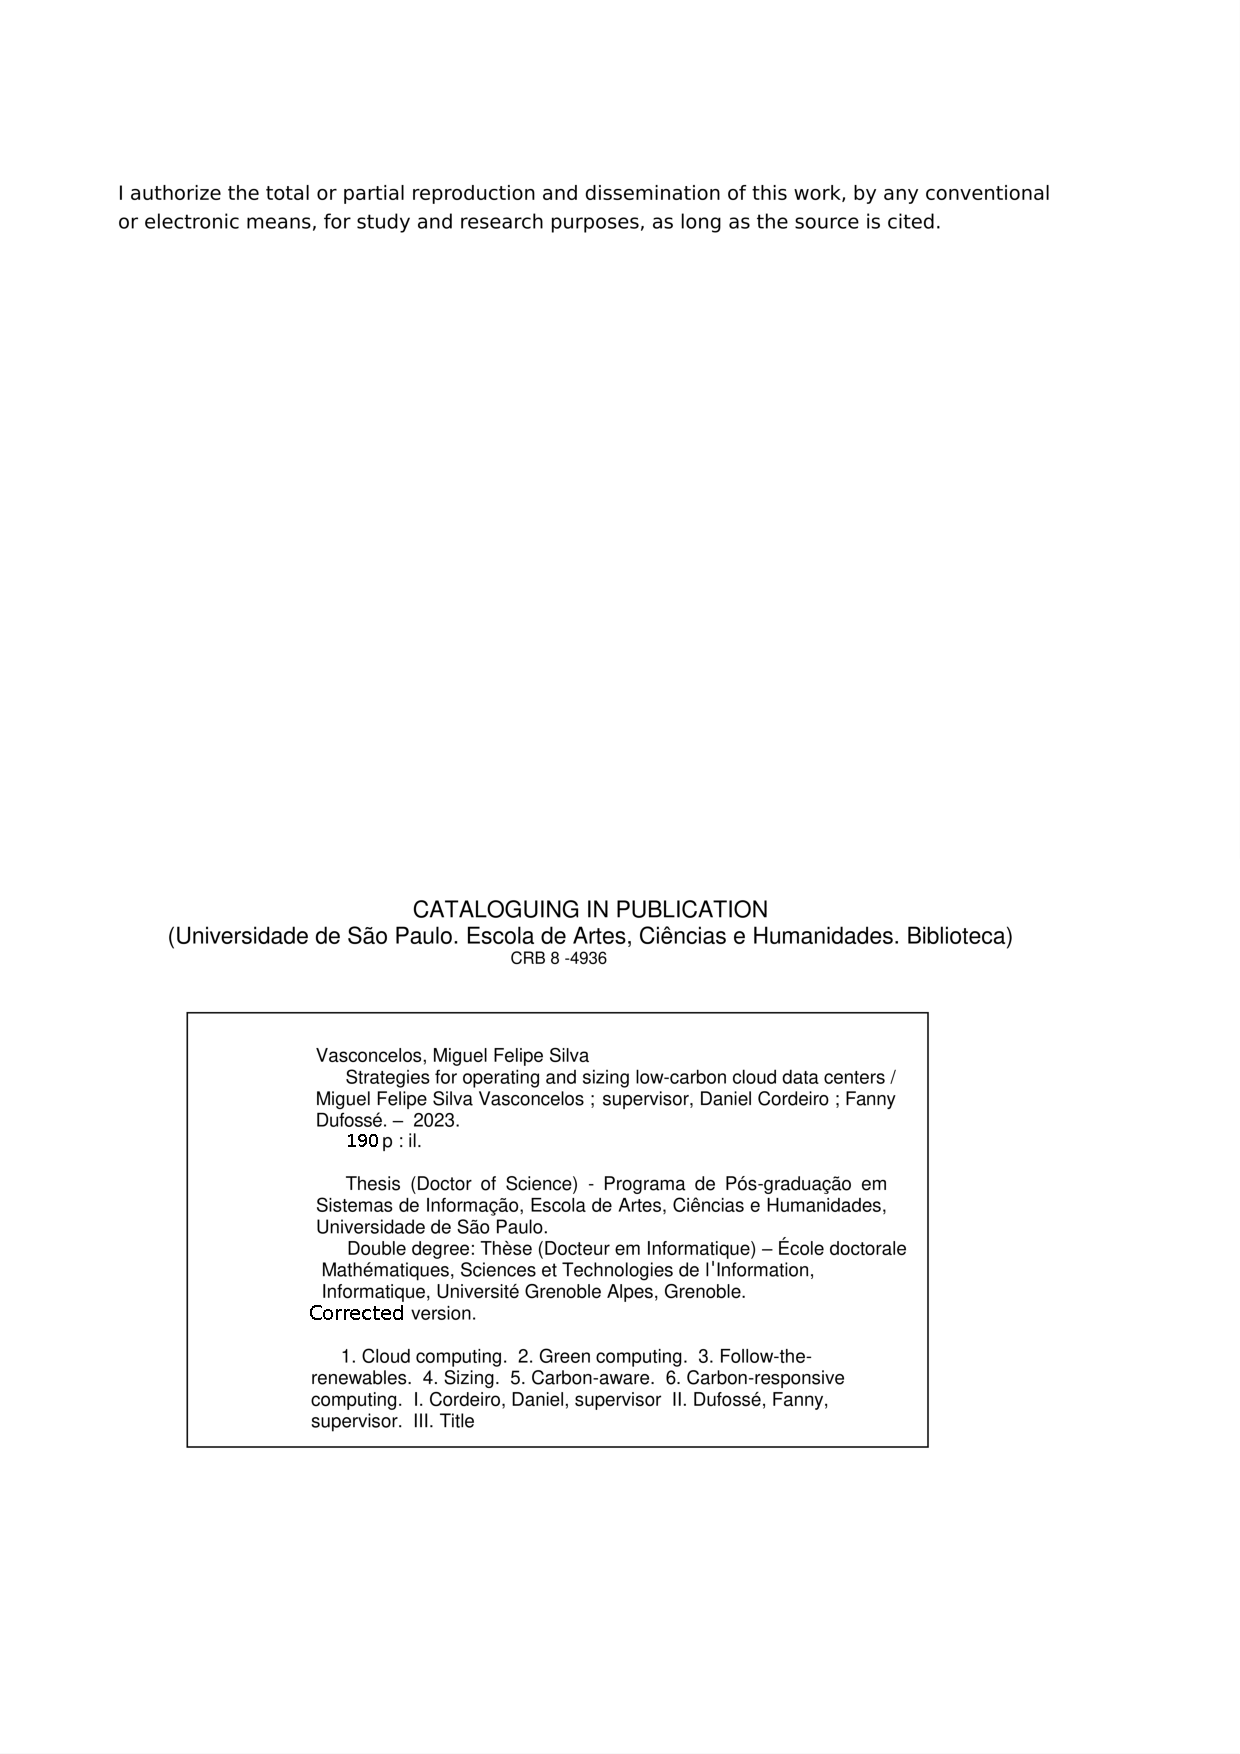
\includepdf{ficha_catalografica_uga.pdf}
\cleardoublepage


\pagestyle{plain}  % display page number only

%!TEX encoding = UTF-8 Unicode

\addchap[Acknowledgments]{%
	\foreignlanguage{french}{Remerciements} {\Large (Acknowledgments)}
}


Agradecer aos meus pais e irmao

meus orientadores

meus amigos do lab e da each

colaboradores do proejto datazero

tb a each e a univ de grenoble, fapesp, labex, pessoal do datazero e td mais







\cleardoublepage

\addchap{Abstract / \foreignlanguage{french}{Résumé}}

\section*{Abstract}

Falar do consumo de energia

impacto ambiental dos dcs

emissao de carbono

tecnicas carbon aware

carbon responsive

sizing e contention

follow the renewables




% -----------------------------------------------------------------------------

\begin{otherlanguage}{french}

\section*{Résumé}

Falar do consumo de energia

impacto ambiental dos dcs

emissao de carbono

tecnicas carbon aware

carbon responsive

sizing e contention

follow the renewables




\end{otherlanguage}

\cleardoublepage

\listoffigures
\cleardoublepage

\listoftables
\cleardoublepage

\setcounter{tocdepth}{3}  % define depth of ToC
\phantomsection\addcontentsline{toc}{chapter}{{\contentsname}}  % display ToC to ToC
\tableofcontents
\cleardoublepage

% --- MAIN MATTER ----------------------

\pagenumbering{arabic}  % arabic page numbering (e.g., 1 2 3), reset counter
%\pagestyle{scrheadings}  % display header and footer
\addtocontents{toc}{\bigskip}  % visual hint for numbering change in ToC

% main chapters go here
%==============================================
%==============================================================================

\chapter{Introduction} 
\label{chap:intro}


Cloud computing has revolutionized the industrial and academic world of Information Technology with its ability to provide large amounts of computing resources on demand. Most of the applications and services we use every day that feature more and more users, such as social networking, e-mail, video games, internet banking, health applications, and video streaming, are supported by cloud computing platforms.

Despite all its benefits, cloud data centers (DCs)---the facilities that host all the infrastructure needed for the cloud---have a significant power demand. The International Energy Agency (IEA) estimates that the data centers that host cloud computing platforms consumed between 240 to 320 TWh, or approximately 1\% of the global final electricity generated in 2022~\cite{IEA_2022}. To put this energy consumption into perspective, it's enough to supply the annual energy demand of entire countries. In 2022, seven countries had an energy consumption similar to the DCs energy demand: Greece (316 TWh), Israel (304 TWh), Belarus (297 TWh), Switzerland (292 TWh), Hungary (266 TWh), Portugal (258 TWh), and Morocco (257 TWh)~\cite{owidenergy}.


Efforts from both academia and industry alike are trying to reduce this gigantic energy consumption. An analysis of the global energy use by data centers performed by \citet{masanet2020recalibrating} showed that during the period between 2010 and 2018, the DC's internet protocol traffic increased more than 10-fold, it is estimated that the DC's storage capacity increased by 25-fold, and the DCs workload and compute instances increased by 6-fold. On the other hand, the energy consumption only increased by 6\% thanks to improvements in: i) virtualization, which allowed a 5-fold increase in the average number of compute instances per physical server; ii) more energy-efficient servers (a decrease with a factor of 4 regarding the power used for computation and a factor of 9 in terms of watts per terabyte); and iii) energy-efficient infrastructures, in particular for the cooling needs and power supply.

It is uncertain if the improvements in efficiency in cloud computing will mitigate the power increase caused by the growing demand for computational resources in the long term. In the work of~\citet{koot2021usage}, the authors developed a model for forecasting the energy consumption of data centers using the system dynamic models approach. Considering the period from 2016 to 2030, and the scenario with the end of Moore's law---that predicts that the number of components in the integrated circuits doubles every year~\cite{Mack_2011_moorelaw}---and the rise of industrial Internet of Things applications, the energy demand of the data centers could reach 2.3\% of the global electricity generation---it will double considering what was reported by the IEA for the year 2022~\cite{IEA_2022}.

The electricity consumption of the DCs results in an environmental impact in terms of Greenhouse Gases (GHG) emissions. According to the International Energy Agency, 1\% of the energy-related GHG emissions originate from data centers and data transmission networks~\cite{IEA_2022}. The extent of this impact depends on the type of source used to produce the electricity. Table~\ref{tab:co2_power_sources} presents the emissions for the different types of power sources to produce 1 kWh of energy. The emissions are measured using the carbon dioxide equivalent (or \ch{CO2}-eq)  metric. This metric is used to compare different GHGs in terms of their Global Warming Potential (GWP) using carbon dioxide as a base: methane (\ch{CH4}) has a GWP of 25, which means that emitting 1g of \ch{CH4} in the atmosphere has the same environmental impact as emitting 25g of \ch{CO2}~\cite{eurostat_co2_eq}. It is possible to observe that producing power from coal emits 77 times more \ch{CO2} than wind or nuclear. In 2019, approximately 70\% of the internet's data traffic was processed by the DCs in the ``Data Center Alley'', a region located in Virginia (United States of America), which was only supplied by less than 2\% of renewable energy (green energy)~\cite{clicking_clean_virginia}. 

In order to reduce their environmental impact, major cloud providers---such as Amazon AWS, Apple, Google, Meta (former Facebook), and Microsoft---made commitments to integrate low-carbon intensive electricity produced by renewable sources in the operations of their data centers, and some have already deployed their projects to reach the goal of minimizing the carbon footprint. In fact, Google reported that in 2022, 64 percent of the power used to supply its DCs on an hourly basis came from renewable sources~\cite{google_sustainability_report_2023}, with some DCs reaching up to 97\% of green energy usage.

\begin{table}[!ht]

\caption{ Emissions (in g\,\ch{CO2}-eq) from different power sources per kWh of electricity produced~\cite{nrel_lifecycle_2021}.}\label{tab:co2_power_sources} \centering

\begin{tabular}{|l|r|}
  \hline
  \textbf{Generation technology} & \textbf{Emissions ($\mathbf{g\,\ch{CO2}\text{-}eq/kWh}$)}   \\
  \hline  
  Coal   & 1 010\\  
  \hline
  Oil   & 840\\
  \hline
  Natural gas   & 486\\
   \hline
  Biomass   & 52 \\
  \hline
  Photovoltaic   & 43 \\
  \hline
  Hydropower & 21 \\
  \hline
  Nuclear   & 13 \\
  \hline
  Wind   & 13 \\
  \hline
\end{tabular}
\end{table}


The cloud platforms are integrating renewable power into their operations in the following ways. One possibility is to buy green energy from the local electricity grid, although this makes them dependent on the grid's energy mix, and not all locations in the world are supplied by low-carbon sources. Another possibility is to manufacture their own on-site renewable infrastructure. A critical aspect of producing electricity using renewable energy that must be considered for both possibilities,  is their intermittent nature---their production fluctuates over time and is influenced by variables such as the time of day, climate, season, and geographic location. For example, photovoltaic panels (PVs) only produce power when the sun is shining, and during the winter, the solar irradiation is lower than in the summer. For hydropower, long periods without rain will affect power production.

The adoption of energy storage devices (ESDs) in DCs to store renewable energy~\cite{wang2012_EDCS} is an approach to dealing with intermittency. These devices are already used in DCs as a temporary backup for power outages. The green energy from the ESDs could be used when there is no production of green power or when demand is greater than production. Nevertheless, this approach also presents some challenges for deciding when to use or recharge, given the characteristics of the ESDs, such as the self-discharge rate (they lose stored energy over time when not used), aging (their maximum capacity decreases over time), and limited charge and discharge rates (the maximum power that can be extracted or recharged).

In this thesis, we study how to reduce the environmental impact of cloud computing data centers, specifically in terms of \ch{CO2} emissions. The usage of Carbon-Responsive strategies---approaches that are aware of their carbon footprint and use this information to make decisions~\cite{schooler2021carbonaware}---is explored to reduce the \ch{CO2} emissions in both operating and sizing the data centers---determining the required on-site renewable infrastructure (area of solar panels, number of wind turbines, capacity of ESDs). In terms of DC operations, we leverage the workload scheduling using ``follow-the-renewables'' approaches---strategies that migrate and allocate the workload to the locations with higher renewable energy availability~\cite{shuja2016sustainable}---and study their impact on both energy consumption and network congestion. Regarding sizing, we model our problem using a Linear Program (LP) formulation that considers the characteristics of each DC location in terms of cooling needs and local grid energy mix, as well as the fact that the renewable infrastructure generates an environmental impact. More details about the structure and contributions of this thesis are presented in the next section.

\section{Structure of the thesis and contributions}

This thesis is structured into six chapters, which include this introductory chapter. An overview of the content of each chapter and their respective contributions is described in what follows.

In Chapter~\ref{chap:background}, the reader is introduced to the concepts required to comprehend the research done in this thesis. In particular, the chapter contains a description of the general scenario of cloud computing, how one can measure the environmental impact of cloud platforms, an overview of scheduling algorithms in the context of cloud computing, and the definition of carbon-responsive strategies---in particular, the approaches explored in this thesis: ``follow-the-renewables'' and sizing. Finally, the related works used as inspiration or as baselines for our proposed solutions are presented in this chapter as well.


An analysis of adopting the carbon-aware strategy ``follow-the-renewables'' and its impact on energy consumption and network congestion is presented in Chapter~\ref{chap:smartgreens}. The proposed solution consists of an algorithm that considers the network topology and usage for scheduling the workload migration. Through computational experiments with real-world data for the workload, cloud infrastructure, and a simulator that uses realistic models validated by the scientific community for both energy consumption and network usage, the results show that the proposed solution outperforms the baselines considering energy consumption, non-renewable energy consumption and network congestion.

Chapter~\ref{chap:ccgrid} introduces a carbon-responsive strategy that can be combined with follow-the-renewables to reduce the carbon footprint of operating cloud computing platforms: sizing the renewable infrastructure. This strategy involves determining the required area of on-site solar panels and the capacity of the batteries to supply the DCs power demand. The proposed solution consists of a Linear Program formulation that addresses both the workload scheduling using follow-the-renewables and the sizing of the on-site renewable infrastructure. By modeling these two sub-problems as one problem, it is possible to evaluate whether it is more effective to execute the workload in other geographic locations or to increase the area of solar panels and capacity of the batteries to achieve the goal of reducing the \ch{CO2} emissions. The model only uses linear variables, enabling it to be optimally solved in polynomial time---essential for the scale of cloud computing platforms that have millions of servers and execute hundreds of millions of computational tasks daily. Other important aspects of the modeling are that it considers the characteristics of each DC geographic location in terms of cooling needs, the energy mix of the local electricity grid (which may have a share of renewable energy sources), and the fact that manufacturing solar panels and batteries has an environmental impact. The results demonstrate that the hybrid configuration that combines both the on-site renewable infrastructure and the regular grid outperforms in terms of \ch{CO2} emissions the strategies of having a DC only supplied by energy produced from its local renewable infrastructure---a reduction of approximately 30\%---and only using power from the regular electrical grid---a reduction of approximately 85\%.


The model introduced in Chapter~\ref{chap:ccgrid} focuses on the short-term operation (one year). In Chapter~\ref{chap:ccgrid-extension}, we extend the model to evaluate how to minimize the carbon emissions of cloud data center operations in the long term. The following modifications and analysis were performed: the environmental impact of the whole life cycle of the renewable infrastructure (from manufacturing, operation and recycling) is taken into account to make the model closer to the real-world; an analysis of the benefits and challenges of including wind turbines in the on-site renewable infrastructure; an assessment of the model's sensitivity to the inputs, in particular climate conditions and grid emissions data; an analysis of how much the \ch{CO2} emissions can be reduced by adopting the flexibility of delaying a part of the workload, which could be used to mitigate the impacts of over-sizing the renewable infrastructure; a discussion of the monetary costs (in dollars) associated with on-site renewable infrastructure, as well as the trade-offs between minimizing the carbon footprint and reducing the costs for the DCs; and deciding to manufacture new servers over the years that may be more energy-efficient, considering that manufacturing them also emits carbon. This modeling may be used to guide decision-makers in their efforts to reduce the carbon footprint of cloud data centers.

Finally, Chapter~\ref{chap-conclusion} presents a discussion of the main contributions of this thesis, as well as possible future research trajectories.



%============================================================================================================
\chapter{Background and Related Work}
\label{chap:background}

This chapter provides the foundational knowledge required for the reader to comprehend the subsequent chapters of this thesis. First, the general scenario of cloud computing is presented in Section~\ref{sec:cloud}. Section \ref{sec:measuring_environmental_impact} presents how one can measure the environmental impact of cloud computing platforms. Then, an introduction to scheduling in the context of clouds is shown in Section~\ref{sec:scheduling_cloud}.  The existing approaches explored in this thesis to reduce the environmental impact of cloud computing platforms are discussed in Section~\ref{sec:carbon_responsive}, and the works used in this thesis as inspiration and baselines are presented as well. Finally,  Section~\ref{sec:summary_background} summarizes this chapter.
\section{Cloud computing}

\label{sec:cloud}

Cloud computing was introduced by the industry to address the most significant problems of e-commerce found at the time. Before the advent of cloud computing and its on-demand access to computational resources, users and companies had to purchase their own computational infrastructure to deploy their services or applications. In the event of a sudden surge in requests, it was often challenging to scale the computational infrastructure in time to handle the computational load demand. Despite its revolutionary aspects in information technology, cloud computing is not classified as a new paradigm in computer science research. As a matter of fact, it is the evolution of research into different fields of computer science, such as clusters, grids, autonomous computing, and ubiquitous computing.


One of the critical elements that enable cloud computing is virtualization technology, in which the computational resources of a physical machine are converted to virtual resources that can be shared among many users and applications---also known as multi-tenancy.  The main ideas from virtualization originate from the late 1950's and beginning of the 1960's with the multiprogramming paradigm, and today, the research on virtual machines (VMs) and containers continues to investigate the compromises outlined in the literature of multiprogramming in terms of portability---allowing the virtual resource to execute on any hardware,  performance---the impact of the additional virtual layer in the application execution in comparison to the gains regarding multi-tenancy, and security---how to isolate the interaction between different applications and the applications and the computational resources~\cite{randall2020_virtualization}.


Cloud computing platforms generally support services in three distinct levels: IaaS (Infrastructure as a Service), PaaS (Platform as a Service), and SaaS (Software as a Service)~\citep{fos08}. In the first level, Infrastructure as a Service (IaaS), the platform grants users access to hardware resources (such as processing and storage) and charges them for their usage. Services such as Amazon EC2 (Elastic Cloud Computing) Service and Amazon S3 (Simple Storage Service) are examples of IaaS clouds.   At the second level, Platform as a Service (PaaS), the provider supports a complete development, testing, and deployment environment for the application developer, which usually means that the developer will have to follow a specific fixed development model and accept restrictions on how to model the software in exchange for the scalability provided. An example is the Google App Engine. Finally, at the third level, Software as a Service (SaaS), specific applications are offered to users via the Internet, and the rate is proportional to the use of the application. We can cite the  Google Docs office applications as examples.


Modern cloud computing platforms are composed of multiple data centers geographically distributed over the world---also denominated cloud federations or multi-clouds. Figure~\ref{fig:dc_locations} illustrates the locations of the cloud data centers from Microsoft's Azure that, in total, consist of millions of physical servers~\cite{roach2021_microsoftazure}. The need for such geographically distributed infrastructure comes from meeting the demand of the huge number of users and reducing the response time for their applications, as well as for security and redundancy reasons. For example, if a data center in a region goes down because of a power problem or hacking attack, another region could temporarily receive the computational load. Finally, this distributed infrastructure enables exploring different approaches to reduce the environmental impact of operating the data centers, and more details of these strategies are given in Section~\ref{sec:carbon_responsive}.


\begin{figure}[h]
\centering
  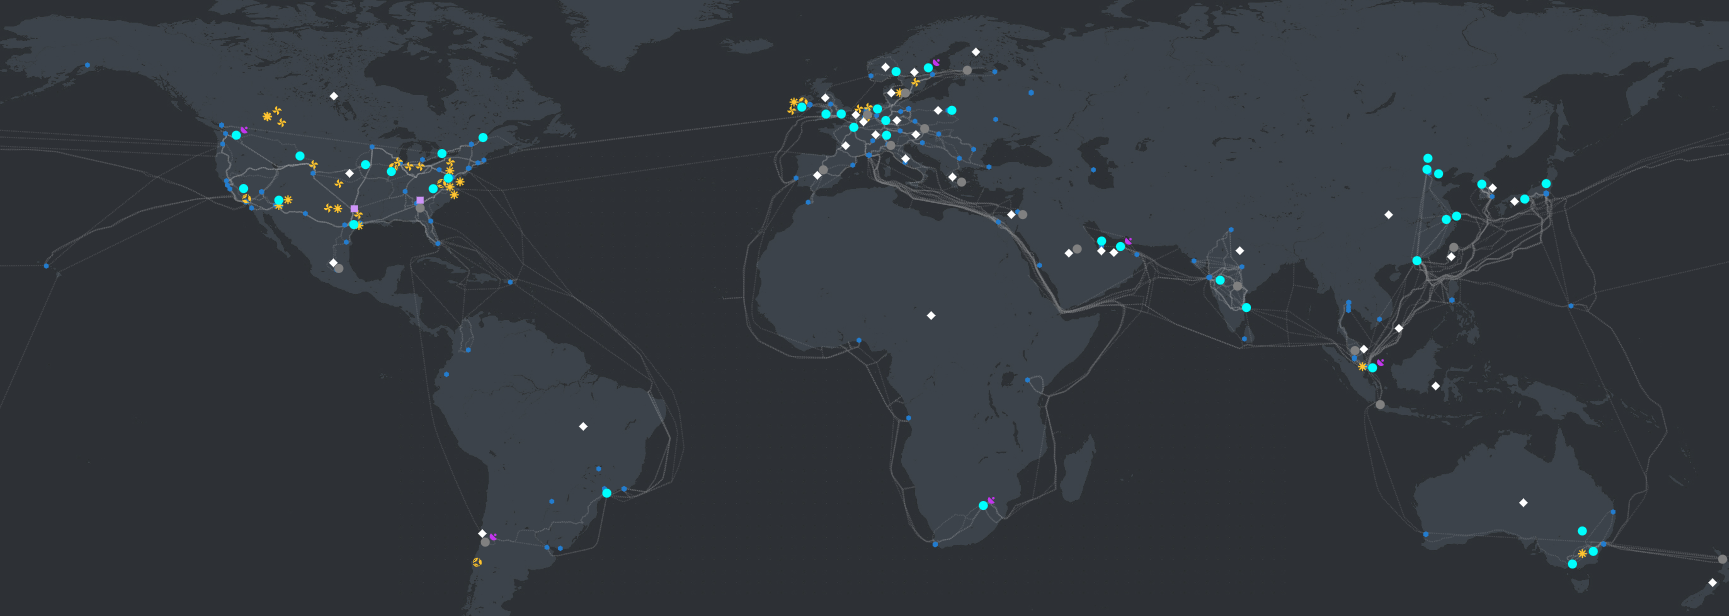
\includegraphics[width=\linewidth]{images/azure_cloud_infra.png}
  \caption{Geographic locations of Microsoft's Azure DCs. Extracted from~\cite{azure_dcs_location}.}
  \label{fig:dc_locations}
\end{figure}

\section{Measuring the environmental impact of cloud computing platforms}

\label{sec:measuring_environmental_impact}


The GHG protocol~\cite{ghgprotocol2004} was developed as a way to standardize the measurement and reporting of companies' environmental impact. It considers six types of Green Houses Gases (GHGs) of the Kyoto protocol: carbon dioxide (\ch{CO2}), methane (\ch{CH4}), sulfur hexafluoride (\ch{SF6}), nitrous oxide (\ch{N2O}), hydrofluorocarbons (HFCs), and perfluorocarbons (PFCs).


The protocol has three scopes to quantify the direct and indirect emissions:

\begin{itemize}
\item \textbf{Scope 1 - Direct GHG emissions}: Takes into account the emissions generated by sources that the company owns or has control over. In the context of cloud computing, it could come from the electricity generated when there is a power surge, and generators should be used as a backup; the transportation of products, materials, employees using the company vehicles; and the cooling of the data center infrastructure~\cite{gupta2021_chasingcarbon}.
\item \textbf{Scope 2 - Electricity indirect GHG emissions}: Takes into account the emissions generated from the electricity consumed.
\item \textbf{Scope 3 - Other indirect GHG emissions}: This one is optional, and takes into account emissions from the production or extraction of materials and fuels bought, for example, IT equipment (such as servers and routers) as well as constructing the data center facilities. Emissions from transportation are also included in this scope if they come from vehicles not owned by the company.
\end{itemize}  

Major cloud players already provide sustainability reports and use the GHG Protocol. In the 2023 sustainability report from Meta~\cite{meta_sustainability_report_2023}, it is estimated that 1\% of the emissions came from Scope 1, less than 1\% from Scope 2, and 99\% from Scope 3. Additionally, it is stated that the operational emissions have been reduced by 94\% in comparison to 2017 thanks to the renewable energy commitments. Another remarkable example is the Google environmental report from 2023~\cite{google_sustainability_report_2023}, where it is estimated that 1\% of the emissions come from Scope 1, 24\% from Scope 2, and 74\% from Scope 3. Google also reports that most of the Scope 3 emissions come from manufacturing the hardware and capital goods they bought and constructing the data center facilities.

In this thesis, the environmental impact is only evaluated in terms of the carbon footprint---using the \ch{CO2} equivalent metric (\ch{CO2}-eq). This decision was taken due to the lack of data for measuring other environmental impacts, such as water usage, and impacts caused by extracting raw minerals to fabricate the integrated circuits.

\section{Scheduling for cloud computing platforms}
\label{sec:scheduling_cloud}

Scheduling problems are combinatorial optimization problems where, given the description of the characteristics of a computational resource set ($\alpha$) and a task set ($\beta$), the objective is to find an allocation (in time) of resources to tasks that minimize some optimization criteria ($\gamma$). These problems are denoted, generally, using the \mbox{$\alpha$ $\vert$ $\beta$ $\vert$ $\gamma$} notation, introduced by Graham~\citep{graham}. 

The most common criterion studied in problems of high-performance computing is called makespan (also denoted by $C_{\max}$), which indicates the time when the last task that makes up an application finishes its execution. When the available computational resources are identical and known previously, and we are interested in minimizing makespan---typically the case in scheduling problems in cluster and computational grids---the problem is strongly NP-hard~\citep{Garey}. This problem is denoted by $P\,\vert\,\vert\,C_{\max}$ in Graham's notation.

For the research problem explored in this thesis, $\alpha$ represents the computational resources (memory and CPU) from the servers of the data centers as well as their information about the availability of low-carbon-intensive power sources, $\beta$ represents the VM requirements in terms of execution time,  deadline, memory and CPU, and $\gamma$ represents the reduction of carbon-intensive energy consumption.

It is known---from the work of~\citet {graham} and~\citet {Garey}---that the class of greedy algorithms known as list algorithms provides fast and efficient heuristics for scheduling tasks on parallel computers. These algorithms have a $2 -1 /m$ approximation guarantee for the worst case, but are remarkably effective in practice, especially when the ratio of the number of tasks to the number of available computational resources is large. Among the most commonly used list algorithms are the Longest Processing Time first (LPT) and Shortest Processing Time first (SPT),  for homogeneous platforms, and the Heterogeneous Earliest Finish Time (HEFT) algorithm, for heterogeneous platforms.

The VM consolidation strategy illustrates an example of a scheduling problem in cloud computing enabled by virtualization. It consists of using live migrations---migrating the VM between different machines while in execution, that is, without preemption---to reallocate the VMs in order to achieve the minimum number of physical machines used, and turning off the machines that became idle to save power. The reader can check the work from~\citet{10.1145/3470972} for a systematic literature review on such techniques.


The greedy algorithms were adopted in some of the solutions proposed in this thesis, as well as most of the related works used as baselines and inspiration. The justification for such a decision is that despite not providing the optimal solution, they can provide an acceptable solution in a reasonable amount of time, which is important considering the workload size with millions of tasks and restrictions such as deadline, response time, and others. The following section presents these strategies to the reader.




\section{Carbon-Responsive Computing}

\label{sec:carbon_responsive}

Many efforts from both academia and industry are being made to reduce the environmental impact of information technology. The term Carbon-Responsive Computing was created to describe the strategies that explore moving the computational workload both in time and spatial dimensions aiming to reduce the carbon footprint of the operation~\cite{schooler2021carbonaware}.


There are three levels of Carbon-Responsive computing. In the first, Carbon-aware computing, the system knows the carbon intensity of the electricity used by its workloads or IT equipment. In the second, Carbon-responsive computing, the information about the carbon intensity is taken into account to make decisions. The final stage, Carbon-resilient computing, studies how to manage and integrate carbon-responsive elements and what modifications are needed in IT and power supply infrastructure to reduce the carbon footprint.

In this thesis, it is presented a study of the Carbon-Aware strategy follow-the-renewables---presented in Section~\ref{sec:followtherenewables}, and the Carbon-Resilient computing strategy of sizing the renewable infrastructure---discussed in Section~\ref{sec:sizing}.

\subsection{Follow-the-renewables}

\label{sec:followtherenewables}

As we saw in Section~\ref{sec:cloud}, modern cloud computing platforms are geographically distributed across the globe, having data centers in many combinations of latitudes, longitudes, and time zones. Considering that each location has a different potential for generating renewable power, and that renewable energy is intermittent---the sun only shines during the day, and the wind does not blow all the time at speeds that are sufficient to turn the wind turbine propeller---the scheduling algorithms can use this characteristic to plan the execution of the workload in the locations that have more availability of green energy. In the literature, the term ``follow-the-renewables''~\cite{shuja2016sustainable} describes this strategy. This strategy focuses on the Scope 2 of the GHG Protocol, as it schedule the workload to the location that uses less carbon-intensive power from renewable sources.

Figure~\ref{fig:ex_follow_the_renewables} is an illustration of a cloud federation's operation that adopts the follow-the-renewable strategy. The cloud federation is composed of nine data centers geographically distributed over the world, and each DC has on-site solar panels to produce green power and can also use power from the regular local electrical grid. The circles represent the locations of the data centers, and the area of the circle represents the power consumption of the DC at that instant of time. The power consumption is directly related to the amount of computational workload being executed by the DC, therefore the circle area also represents the ratio of workload allocated to the DCs. The color represents the electricity source used to supply the DC. The gray layer in the picture represents the division between night and day periods over the globe. One can observe that a higher portion of the workload was allocated to the DCs where renewable energy is being produced: the DCs located where the sun is still shining. This figure was generated from the experiments performed in this thesis. More details can be found in Chapter~\ref{chap:ccgrid}.

\begin{figure}[h]
\centering
  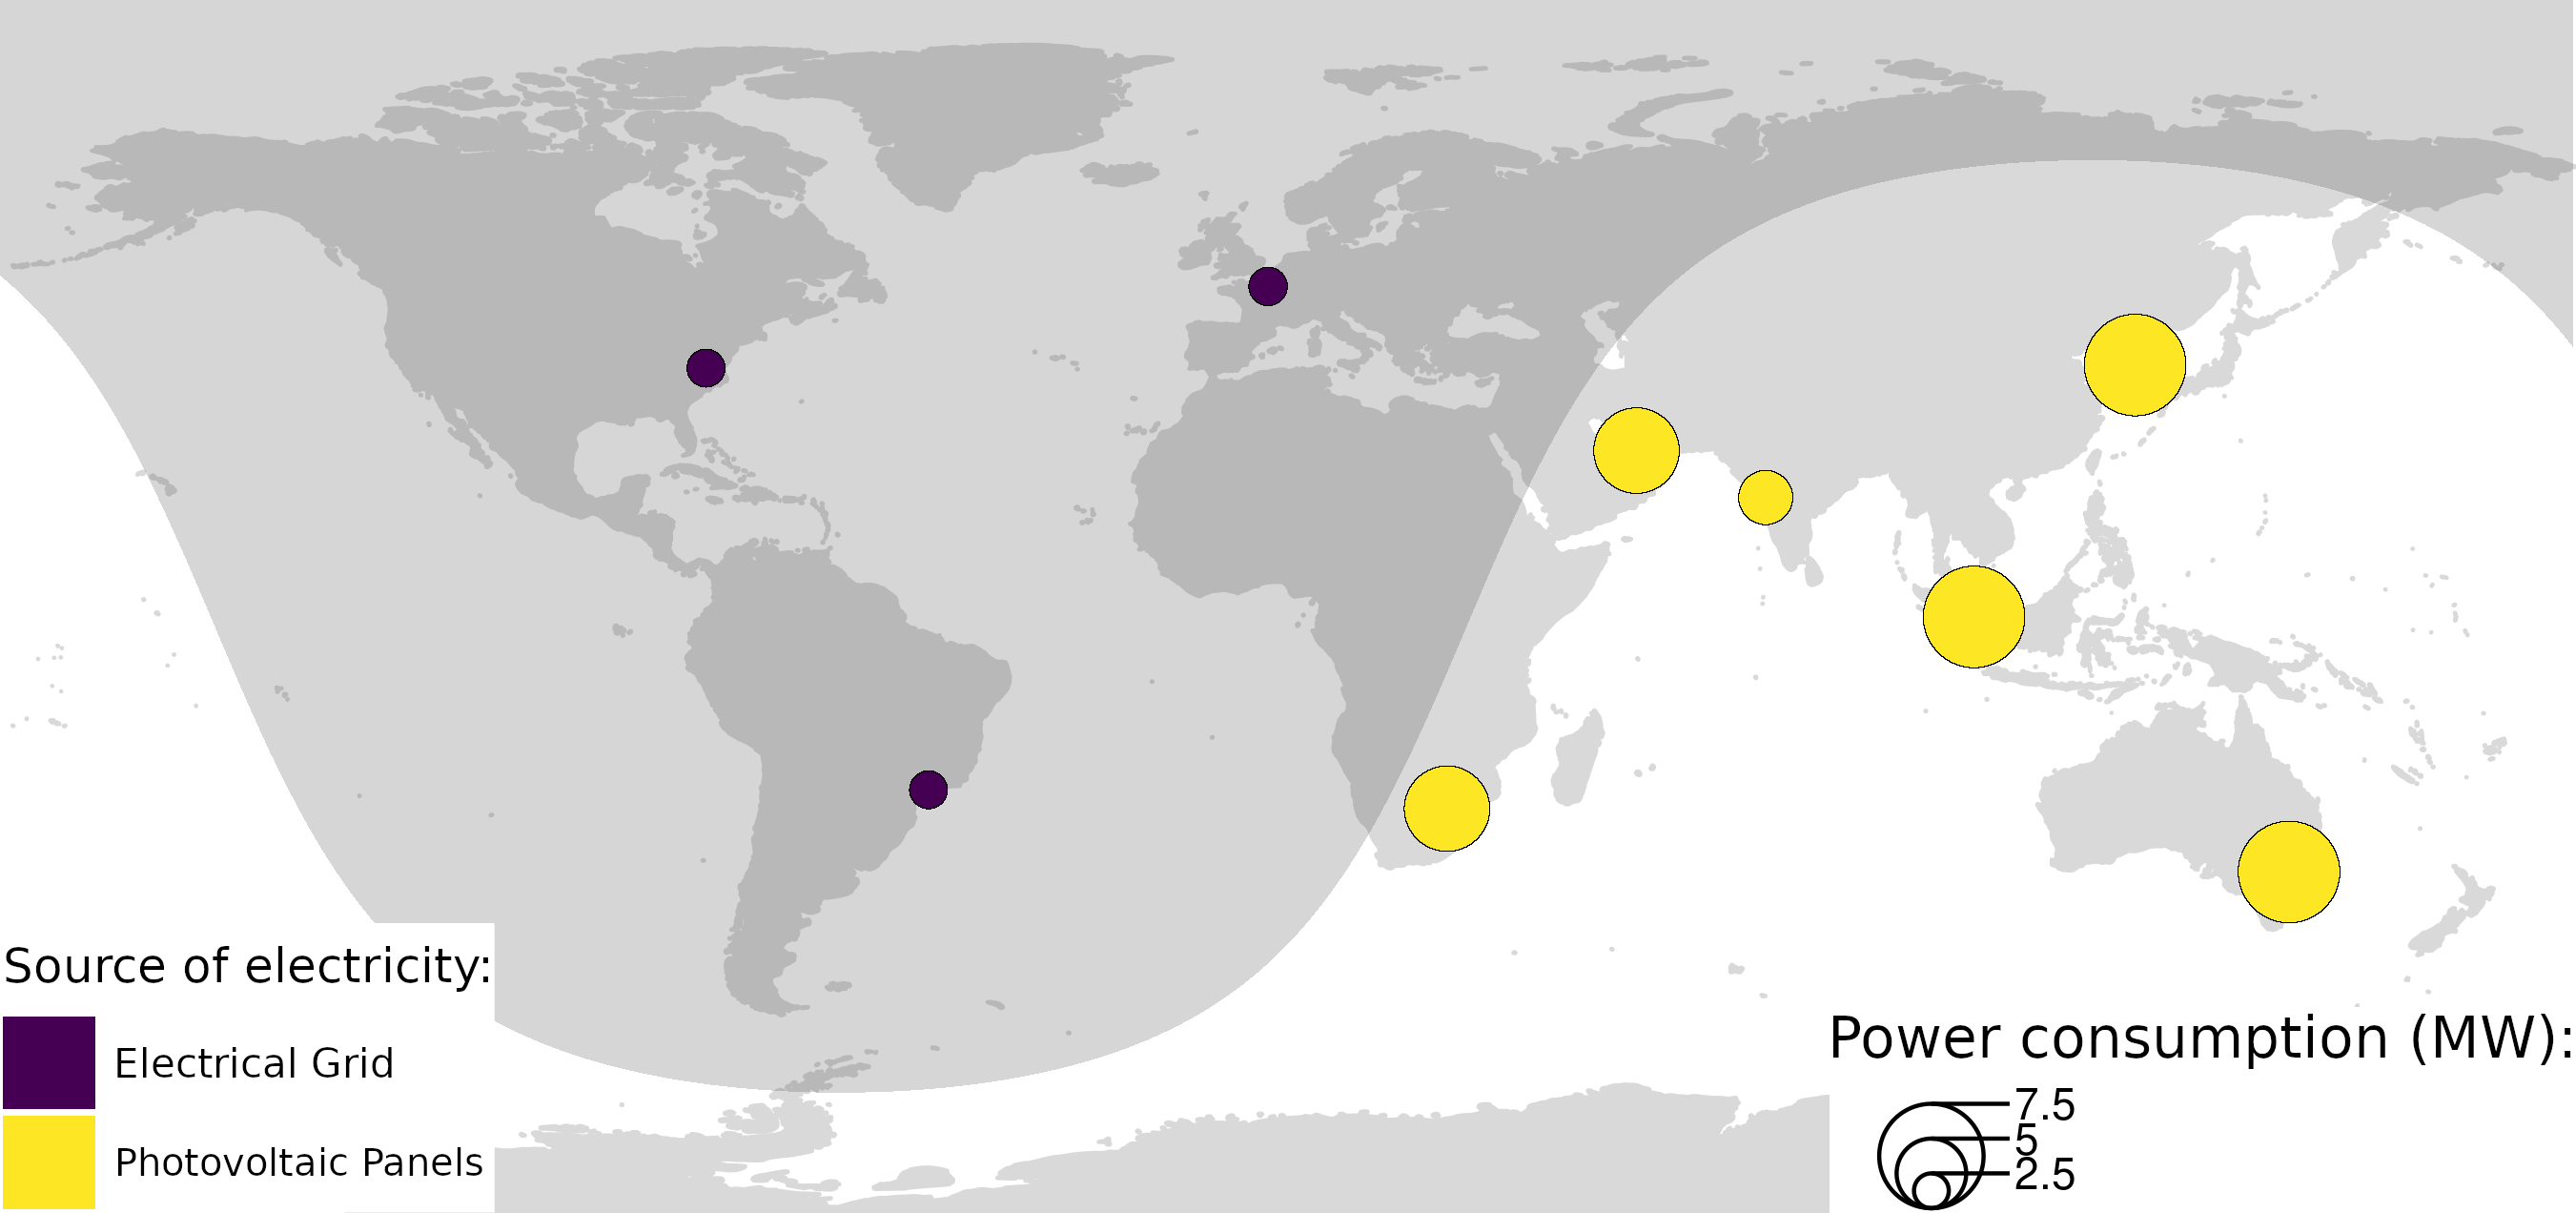
\includegraphics[width=\linewidth]{images/example_follow_the_renewables.png}
  \caption{An example of a cloud federation that adopts the follow-the-renewable strategy. Each circle represents the data center locations: its area represents the total power consumption; the color represents the source of electricity used to supply the DC power demand. The gray layer represents the day and night periods around the world. }
  \label{fig:ex_follow_the_renewables}
\end{figure}


The work from~\citet{XU2020191} provides a comprehensive overview of the classical strategies utilized to reduce data centers' power consumption. Additionally, they present their scheduling algorithm that incorporates the ``follow-the-renewables'' to allocate the workload between the data centers located in different time zones. The optimization algorithm has the objective of minimizing the total carbon emissions of the operation while ensuring the average response time of the requests. The workload will be executed on the data centers they were allocated to, and during execution it is not possible to migrate to other DCs that may have a higher availability of green energy---no VM live migration nor VM consolidation to reduce the number of servers being used.



Reducing power consumption, the environmental impact generated by using carbon-intensive electricity, and monetary costs while not degrading workload performance were studied by~\citet{ALI2021110907}. They proposed a distributed scheduling algorithm for geographically distributed DCs with heterogeneous hardware. The algorithm has two main steps that adopt greed heuristics. The first consists of allocating the workload to the servers given a policy (lower energy price or carbon intensity). In the second step, it is possible either to apply server consolidation to the workload in execution to reduce the number of servers in utilization (by using intra-DC migrations) or the tasks can be shifted to other data centers (inter-DC migrations) in order to use cheaper or greener electricity. The algorithm also considers that the migration's destination server might be less powerful than the server where the tasks were originally in execution, which would degrade the performance of the workload.

\citet{RUIZDUARTE2023_operation_dcs_renewables} studied the problem of operating data centers geographically distributed across the United States in terms of scheduling the workload and the power supply---that comes from the regular electrical grid, batteries, or on-site renewables. The proposed solution consisted of a Mixed Integer Linear Program (MILP) formulation that adopted follow-the-renewables for allocating and migrating the workload, and managed the decision of selecting which power source would be used. The objectives of the MILP are to minimize both costs---that originate from purchasing electricity from the grid, energy storage devices, or selling or buying carbon credits---and \ch{CO2} emissions---that originate from using carbon-intensive electricity from the regular electrical grid.

In~\citet{KHODAYARSERESHT2023_energycarbonaware_vm}, the authors study the workload scheduling problem to minimize energy consumption while avoiding violating the Service Level Agreements. The proposed solution used greedy heuristics to find the server that could run the tasks with the minimum increase in total energy consumption. If the algorithm found more than one server available, the criteria of the one that uses less carbon-intensive electricity was used to break the tie. Therefore, minimizing the emissions was the secondary objective of the algorithm, and the ``follow-the-renewables'' was only applied at this step. It is important to remind the reader that minimizing energy consumption and carbon emissions are different problems. For example, suppose DC A uses power from a grid supplied by coal power plants. In that case, it will have a carbon footprint more than 20 times higher than a DC B that consumes the same amount of power and uses photovoltaic energy--- 1001 g of\ch{CO2}-eq per kWh of electricity produced for coal power and 43  g of \ch{CO2}-eq per kWh for solar power~\cite{nrel_lifecycle_2021}. 

The studies by Camus et al.~\cite{SCORPIOUS,NEMESIS,SAGITTA} aim to optimize low-carbon intensity energy usage in the context of data centers that have a power supply for both the regular electrical grid and locally installed solar panels. Also, these studies consider data centers that are geographically distributed, which allows for exploring ``follow-the-renewables'' strategies. The first study proposed the SAGITTA algorithm~\citep{SAGITTA}, which uses a stochastic approach to estimate renewable energy production and a greedy heuristic to allocate resources to meet the demand of virtual machines. The greedy heuristic chooses which servers in the data centers will receive the virtual machine workload considering their green energy availability and turns off those not selected to reduce the loss of renewable energy. After determining the servers to turn on or off, the algorithm tries to migrate the workload between servers in distinct data centers to use those with the most green energy availability. 

The NEMESIS algorithm~\citep{NEMESIS} is an evolution of the SAGITTA algorithm, and also uses a stochastic approach to estimate renewable energy production and greedy heuristics for VM allocation that select the servers from the data centers with the most available green energy. The main differences are that the proposed solution uses a consolidation algorithm to reduce the number of powered servers and a VM migration algorithm that considers network costs. 

The SCORPIOUS algorithm~\citep{SCORPIOUS} is an extension of the NEMESIS algorithm with a new approach: sharing excess renewable energy generated by geographically distributed data centers that have on-site solar panels installed. This approach uses SmartGrid's collective self-consumption, and the excess of green energy can be used by data centers that are not generating solar power, or when the demand is greater than the production.


Finally, ``follow-the-renewables'' approaches are feasible candidates for mitigating the intrinsic intermittent nature of renewable power, but one must not neglect its limitations. Chapter~\ref{chap:smartgreens} presents a discussion of the impact of adopting such strategies, in particular on the network and energy consumption, a proposed solution that extends the work from~\citet{NEMESIS}, and the works of~\citet{XU2020191} and~\citet{ALI2021110907} were used as baselines to evaluate the solution.


\subsection{Sizing the renewable infrastructure}


\label{sec:sizing}


There are two main options for supplying the cloud federation's power demand with low-carbon-intensive electricity. The data center owner can purchase green power from the local electricity grid that has the integration of renewables---which makes them dependent on the grid, and not all locations provide this possibility---or it can install a local renewable infrastructure in the DCs. For the latter option, the main problem is deciding the dimensions of the renewable infrastructure needed, for example, the required area of solar panels, number of wind turbines, and capacity of the batteries  (to store green power and use it when opportune) to supply the data center and minimize its carbon footprint. This problem is known as \emph{sizing}, \emph{dimensioning}, or \emph{capacity planning} in the literature. Many factors need to be considered in the sizing decision: the costs of manufacturing and operating these devices, the potential of generating power given the climate conditions and the geographic location, and the fact that these devices also present an environmental impact during their lifetime cannot be neglected as well.

The strategy sizing of the renewable infrastructure considers the Scope 1, 2, and 3 of the GHG Protocol: the direct carbon emissions from generating electricity in the DC, emissions from consuming power from the regular electrical grid, and other indirect GHG emissions that come from the manufacturing and life cycle of the renewable infrastructure and IT equipment.


Most of the scientific literature on the sizing problem for cloud data centers has focused on the scenario of a single DC. Two main approaches are investigated: i) the data center may be supplied by the regular electrical grid as a backup when the renewable power production is not sufficient, and ii) the DC is fully supplied by green energy from its on-site renewable infrastructure---which may require the adoption of energy storage devices.


The first approach---using the regular electrical grid as a backup---is adopted by the majority of works on sizing for clouds. To supply the power demand of fog DCs in a rural area in India,~\citet{padma2021_fogdcs_rural} proposed a solution that adopts a Particle Swarm Optimization strategy for sizing a smart microgrid. The optimization problem's objective is to minimize the monetary costs of buying solar panels, wind turbines, diesel generators, and batteries. Additionally, the authors propose a scheduling algorithm to maximize low-carbon-intensive energy utilization from its local renewable infrastructure. % https://doi.org/10.1007/s11276-019-02207-z

Depending on the local electricity grid and the renewable infrastructure, more renewable power can be produced than what the electrical grid can receive. In this situation, there is a curtailment, a reduction in the energy delivered when the generation exceeds the demand or there are system conditions in the grid, such as transmission congestion, minimum generation levels of thermal generators or hydropower, or back-feeding in the distribution systems~\cite{curtailment_def_2021}. 

\citet{Niaz2022_curtailment} evaluated using curtailed green energy to supply the DCs power demand and provide hydrogen to hydrogen refueling stations. The proposed solution consisted of an optimization problem that used Mixed Integer Linear Programming (MILP) with the objective of minimizing the capital costs. The modeling included natural-gas-powered combined cooling, heating, power systems, electrolyzers, hydrogen fuel cells, heat pumps, hydrogen tanks, and battery energy storage systems. The study provided three interesting results: i) the worst scenario regarding both economic and environmental aspects was to only consume power from the regular electrical grid; ii) The scenario with the minimal monetary costs was the combination of using curtailed renewable energy and power from the grid; and iii) the best solution for the environment was to consume only renewable power, however, it resulted in the highest costs.


The second main approach---using only power from the on-site renewable infrastructure without accessing the grid---is becoming more and more explored in the literature, presenting promising results. A planning methodology for a net-zero energy system---an energy system that does not emit carbon dioxide to the atmosphere~\cite{netzero_energy_system}---was discussed by~\citet{Richter2021_netzero_dcs}, which assessed the potential for a net-zero energy DC in Germany through a qualitative study. The data center is considered net-zero because its power demand would only be supplied by electricity generated by the low-carbon-intensive on-site renewable infrastructure. Power from the regular electrical grid is assumed to be highly carbon-intensive and is only used in the case of failures of the green power infrastructure. The research concluded that the DC presented a large potential to operate as a net-zero energy system, taking into account the importance of selecting proper technologies for producing electricity, increasing energy efficiency, and optimal sizing of energy storage devices. Other secondary benefits are that the marketing image and economic value can increase when the DC operates as a net-zero energy system. 

The DATAZERO~\citep{datazero} project explores the possibility of a single data center being operated exclusively from renewable energy and uses energy storage devices to try to smooth the short- and long-term intermittency. The work from~\citet{HADDAD2021100505}---part of the DATAZERO project---evaluates the possibility of using the combination of solar panels and wind turbines for supplying the DC power demand and the usage of batteries and hydrogen storage---for short- and long-term storage, respectively. The study discussed the impact of the geographic location and the computational workload that must be executed in the resulting sizing---number of servers, dimensions of the renewable power sources, and capacity of the energy storage devices.

Another work from the DATAZERO project evaluated how to reduce oversizing, that is, manufacturing more renewable infrastructure than needed, in DCs powered by green energy~\citep{manal2022}. The classical sizing approaches are very sensitive to variations in the inputs, as there are a few days when there is a peak in computational demand for the workload or low renewable production. The proposed solution evaluated how to minimize the oversizing and the impact in terms of Quality of Service and on the dimensions of the renewable infrastructure. A binary search strategy was adopted to find the best relevant sizing, in contrast to the previous studies that used MILP approaches.

Other research areas explored in the scientific literature analyze the sizing of particular elements, such as the electrical infrastructure. ~\citet{sheme2018_batsize} investigated the usage of batteries as an energy storage device and their size to supply 50\% of the DC's total energy demand using power from renewable sources. For the experiments, the authors developed a simulator that receives information on the PV area and capacity of the batteries as input, and different geographic locations were considered: Finland, Crete, and Nigeria. The results highlight the different potential of the geographic locations: Nigeria presented the smallest area of solar panels required: 17\% less than Crete and 45\% less than Finland. Additionally, Finland requires a battery with 39 times more capacity than Nigeria---even if it receives 15\% less solar energy, and Crete needs a battery with a capacity 27\% higher than Nigeria.

Most studies in the literature focus on dimensioning the renewable infrastructure for a single data center. A similar trend can be observed in the context of scheduling problems for DCs powered by green energy:  a literature review on recent publications on the subject of DCs that are supplied by renewable energy was made by~\citet{SONG2022326}, and the results show that over 100 publications, only around 25\% considered geographically distributed data centers partially powered by renewable energy. Additionally, the authors reported that most research on integrating renewable sources in cloud data centers focuses on the scheduling of the workload, and few articles analyze the dimensioning of the renewable infrastructure.

The Carbon Explorer framework~\cite{acun2022holistic} explored sizing for multiple geographically distributed DCs. The study's objective is to supply DCs located in the United States exclusively with renewable power, and three strategies were used: i) only use green power; ii) use renewable power and energy storage devices; and iii) use green energy and workload scheduling. It is assumed that the DCs have access to low-carbon intensive power from the regular electrical grid---solar, wind, or both---and additional renewable infrastructure will be built---PV panels, wind turbines, and batteries, taking into account the emissions of manufacturing. The study performed an exhaustive search to evaluate the possible scenarios. In conclusion, the authors report that, when taking into account the scenario of geographically distributed data centers and the manufacturing carbon emissions of the renewable infrastructure, there may be better solutions than powering the cloud federation exclusively with green power. Finally, deciding the optimal solution is still an open research question for future work.


This thesis explored the dimensioning of geographically distributed data centers worldwide. The proposed solution combined both ``follow-the-renewables'' for scheduling the workload and sizing the renewable infrastructure to reduce the carbon footprint of a global cloud federation. Compared to the Carbon Explorer framework, our proposed solution considers the use of the local electrical grid when feasible, given that it may have the presence of low-carbon-intensive power sources. Finally, our model uses a linear program formulation, in contrast to most of the works in the literature that use MILP.

In Chapter~\ref{chap:ccgrid}, the reader is introduced to our initial modeling of the problem and the evaluation of the short-term scenario (1 year) for reducing the carbon footprint of operating a cloud federation. In Chapter~\ref{chap:ccgrid-extension}, an extension of the modeling is presented, focusing on the long-term operation, taking into account the life-cycle of the renewable infrastructure, another source for renewable power, scheduling strategies to reduce the carbon footprint further, and manufacturing servers taking into account their carbon footprint. Additionally,  one new dimension of the problem is explored: the monetary costs of reducing the environmental impact with on-site renewable infrastructure.




\section{Summary}
\label{sec:summary_background}
This chapter presented an overview of the context of cloud computing, how it is possible to measure the environmental impact of the cloud computing platforms using the GHG protocol, scheduling, and the concept of carbon-responsive computing to describe the strategies for reducing its environmental impact, in particular the follow-the-renewables and the sizing that are explored in this thesis. The content presented in this chapter should provide the reader with adequate information to comprehend the succeeding chapters of this thesis.



%=========================================================================================

%============================================================================================================
%\chapter{Work of smartgreens}
\chapter[Impact of the follow-the-renewables approaches in energy consumption]{Impact of the follow-the-renewables approaches in energy consumption\footnotemark}
\label{chap:smartgreens}

\section{Introduction}

The ``follow-the-renewables'' approach (the reader may consult Chapter 2 for more details) is an interesting strategy for mitigating the intermittency of renewable energy availability without the need to use energy storage devices, for example, when is night in the location where a DC A resides, the workload could be migrated to another DC B where the sun is still shining to use solar power. However, this strategy also has some limitations. First, the process of migrating a job between different DCs consumes energy itself: it uses network devices (such as switches and routers) and a computational task for the live migration process. The scheduling algorithm must consider this energy consumption before deciding if the migration is advantageous. Second, the network communications links that connect the servers inside the DC and the different DCs can suffer from congestion, which may increase migration duration. This results in unnecessary computation and energy consumption on both the origin and the target server: the server that is sending the job needs to wait for the migration process to finish to free its resources and receive additional jobs, or it could be turned off as well to save energy; and the server that is receiving the job will only start executing the new job after the end of the migration process. An efficient scheduling algorithm must consider those factors to decrease the carbon footprint of the DCs operations.

The work by \citet{SAGITTA,NEMESIS} studied the scheduling of the cloud workload, in the form of virtual machines (VMS), on geographically distributed DCs to minimize non-renewable energy consumption. It proposed different stochastic models to estimate renewable energy production and greedy heuristic algorithms to allocate tasks to servers. VMs are allowed to be migrated during the execution to a computer within the same DC (intra-DC server consolidation)  or to a computer in DC located in another geographic location (``follow-the-renewables''). The scheduling algorithm considers the network cost of the migration.

This chapter presents an extension of this work with an analysis of the indirect impact of using the follow-the-renewables approach in energy consumption. This impact can be divided into two: direct and indirect. The network devices' energy consumption causes the direct impact, and the power consumption is considered static since it does not vary significantly based on the device usage ~\cite{energy_network_devices}. For the indirect impact, it is generated by the live migration of the jobs, which uses the network to transfer all the data related to the task to the destination machine, as well as a computational task required to perform this live migration. More specifically, this chapter presents the following contributions:

\begin{itemize}
    \item an analysis of the impact of not considering the network (bandwidth, latency, and topology) in both the energy consumption and network congestion
    \item an accurate estimation algorithm for the time it takes to migrate a virtual machine that takes into account the network topology, links bandwidth, and latency
    \item a scheduling algorithm for the live migration of the jobs that uses the estimation algorithm and has the same or lower brown energy consumption than the baselines, with no network congestion
\end{itemize}


The work of this chapter resulted in the following publication:  \textit{\textbf{Vasconcelos, M. F. S.}, Cordeiro, D., and Dufossé, F. (2022). Indirect network impact on the energy consumption in multi-clouds for follow-the-renewables approaches. In Proceedings of the 11th International Conference on Smart Cities and Green ICT Systems — SMARTGREENS, pages 44–55. INSTICC, SciTePress}. The text of the present chapter is an adaptation of this publication.

This chapter is organized as follows. In Section~\ref{sec:nemesis}, the model of \cite{NEMESIS}, the foundation of this work, is summarized. Section~\ref{sec:modeling_smargreens} details the new scheduling method for the migrations, while Section~\ref{sec:simulations_smargreens} is devoted to simulations parameters. Results are detailed in Section~\ref{sec:results_smargreens}. Finally, Section~\ref{sec:conclusion_smargreens} summarizes the chapter.


\section{The NEMESIS modeling}
\label{sec:nemesis}

The resource management framework NEMESIS~\cite{NEMESIS} manages a multi-cloud composed of DCs geographically distributed across a country. The DCs power demand is supplied from the regular electrical grid and locally installed PVs. Given the intermittency of renewable energy, the NEMESIS algorithm uses the stochastic modeling of SAGITTA \cite{SAGITTA} for obtaining the expected value of the renewable energy available at a given time to be used as input for the scheduling algorithms.

NEMESIS has a central controller, and the workload execution is scheduled at time slots of 5 minutes. The workload consists of heterogeneous VMs in terms of the number of CPU cores, RAM size, and requested execution time. The scheduling decision uses greedy heuristics inspired by the Best-Fit algorithm. While it may not result in the optimal solution, greedy heuristics can provide an acceptable result in a reasonable amount of time, and these characteristics are relevant for the scenario of cloud computing with millions of jobs submitted per hour and a significant portion of these tasks have strict quality of service requirements and cannot be delayed. The scheduling algorithm has four main steps detailed as follows. 

In the first step of the algorithm (pre-allocation of the incoming VMs), the controller will search for servers to allocate the VMS received during the time slot. There are two restrictions for this scheduling algorithm: i) the server has available computational resources to host the VM;  and ii) executing the VM in this server would result in the minimum increase in the expected brown energy consumption. The algorithm first sorts the VMs by their volume (a product of the number of CPU cores and the amount of RAM) in decreasing order and then performs the search for each of the VMs. If a server is found that respects the two restrictions, the algorithm makes a reservation (pre-allocation) for the VM being analyzed and goes to the next VM. On the other hand, if no server is found, the VM will be delayed to be processed in the next time slot.

The second step of the algorithm (revision of the pre-allocations) performs a revision of the reservations made by the previous step, given that the greedy heuristic used may not provide the optimal solution.  The strategy is to move the reservation from the DCs expected to consume more brown energy to the DCs expected to have the most availability of green energy.  There are two constraints for this algorithm: i) there exists a server in the DC being evaluated that can host the VM; and ii) the expected brown energy is reduced.

The availability of green energy may change during the execution of the VMs, and the third step of the algorithm (migration of the running VMs) aims to reduce brown energy consumption by migrating the running VMs. It uses the same strategy as the second step of the algorithm (moves the workload from DCs using more brown power to DCs that have more green power available) and with the following restrictions: i) the migration needs to finish before the beginning of the next time slot; ii) the remaining execution time of the VM needs to be greater than the duration of the migration process; iii) one DC can only migrate to another 2 DCs during a time slot; and iv) the migrations from one DC are planned to execute one after another, that is, they cannot happen simultaneously in parallel. Restrictions (iii) and (iv) are simple heuristics to avoid network congestion with the load generated by the VM live migrations.

The availability of green energy may change during the execution of the VMs, and the third step of the algorithm (migration of the running VMs) aims to reduce brown energy consumption by migrating the running VMs. It uses the same strategy as the second step of the algorithm (moves the workload from DCs using more brown power to DCs that have more green power available) and with the following restrictions: i) the migration needs to finish before the beginning of the next time slot; ii) the remaining execution time of the VM needs to be greater than the duration of the migration process; iii) one DC can only migrate to another 2 DCs during a time slot; and iv) the migrations from one DC are planned to execute one after another, that is, they cannot happen simultaneously in parallel. Restrictions (iii) and (iv) are simple heuristics to avoid network congestion with the load generated by the VM live migrations.


\subsection{Cloud Modeling}\label{sec:cloud_model}

NEMESIS cloud modeling is based on a real cloud infrastructure: the Grid'5000 testbed\footnote{https://www.grid5000.fr}. It is considered a subset of the original platform with 1035 servers distributed among 9 data centers in France and Luxembourg: 116 servers in Grenoble; 74 servers in Lille; 38 servers in Luxembourg; 103 servers in Lyon; 240 servers in Nancy; 44 servers in Reims;  129 servers in Rennes;  151 servers in Sophia Antipolis; and 140 servers in Toulouse. The servers are considered homogeneous in terms of memory, CPU, and energy consumption, and are based in the Taurus node of the Grid'5000, equipped with two Intel Xeon E5-2630 CPUs (6 cores per processor), and 32 GB RAM.

Regarding the network, it is modeled both the connection of the servers inside the DCs (network links with 1 Gbps of bandwidth) as well as the connection between the different DCs  (network links with 10 Gbps bandwidth). Figure \ref{fig:topology} presents the cloud platform's network topology (the DCs' placement was not based on their geographic location but to visualize the network links better). One can observe that multiple DCs share some network links, thus the migration planning needs to consider this information to avoid generating network congestion and the resulting waste of resources.

\begin{figure}[ht]
  \centering
   {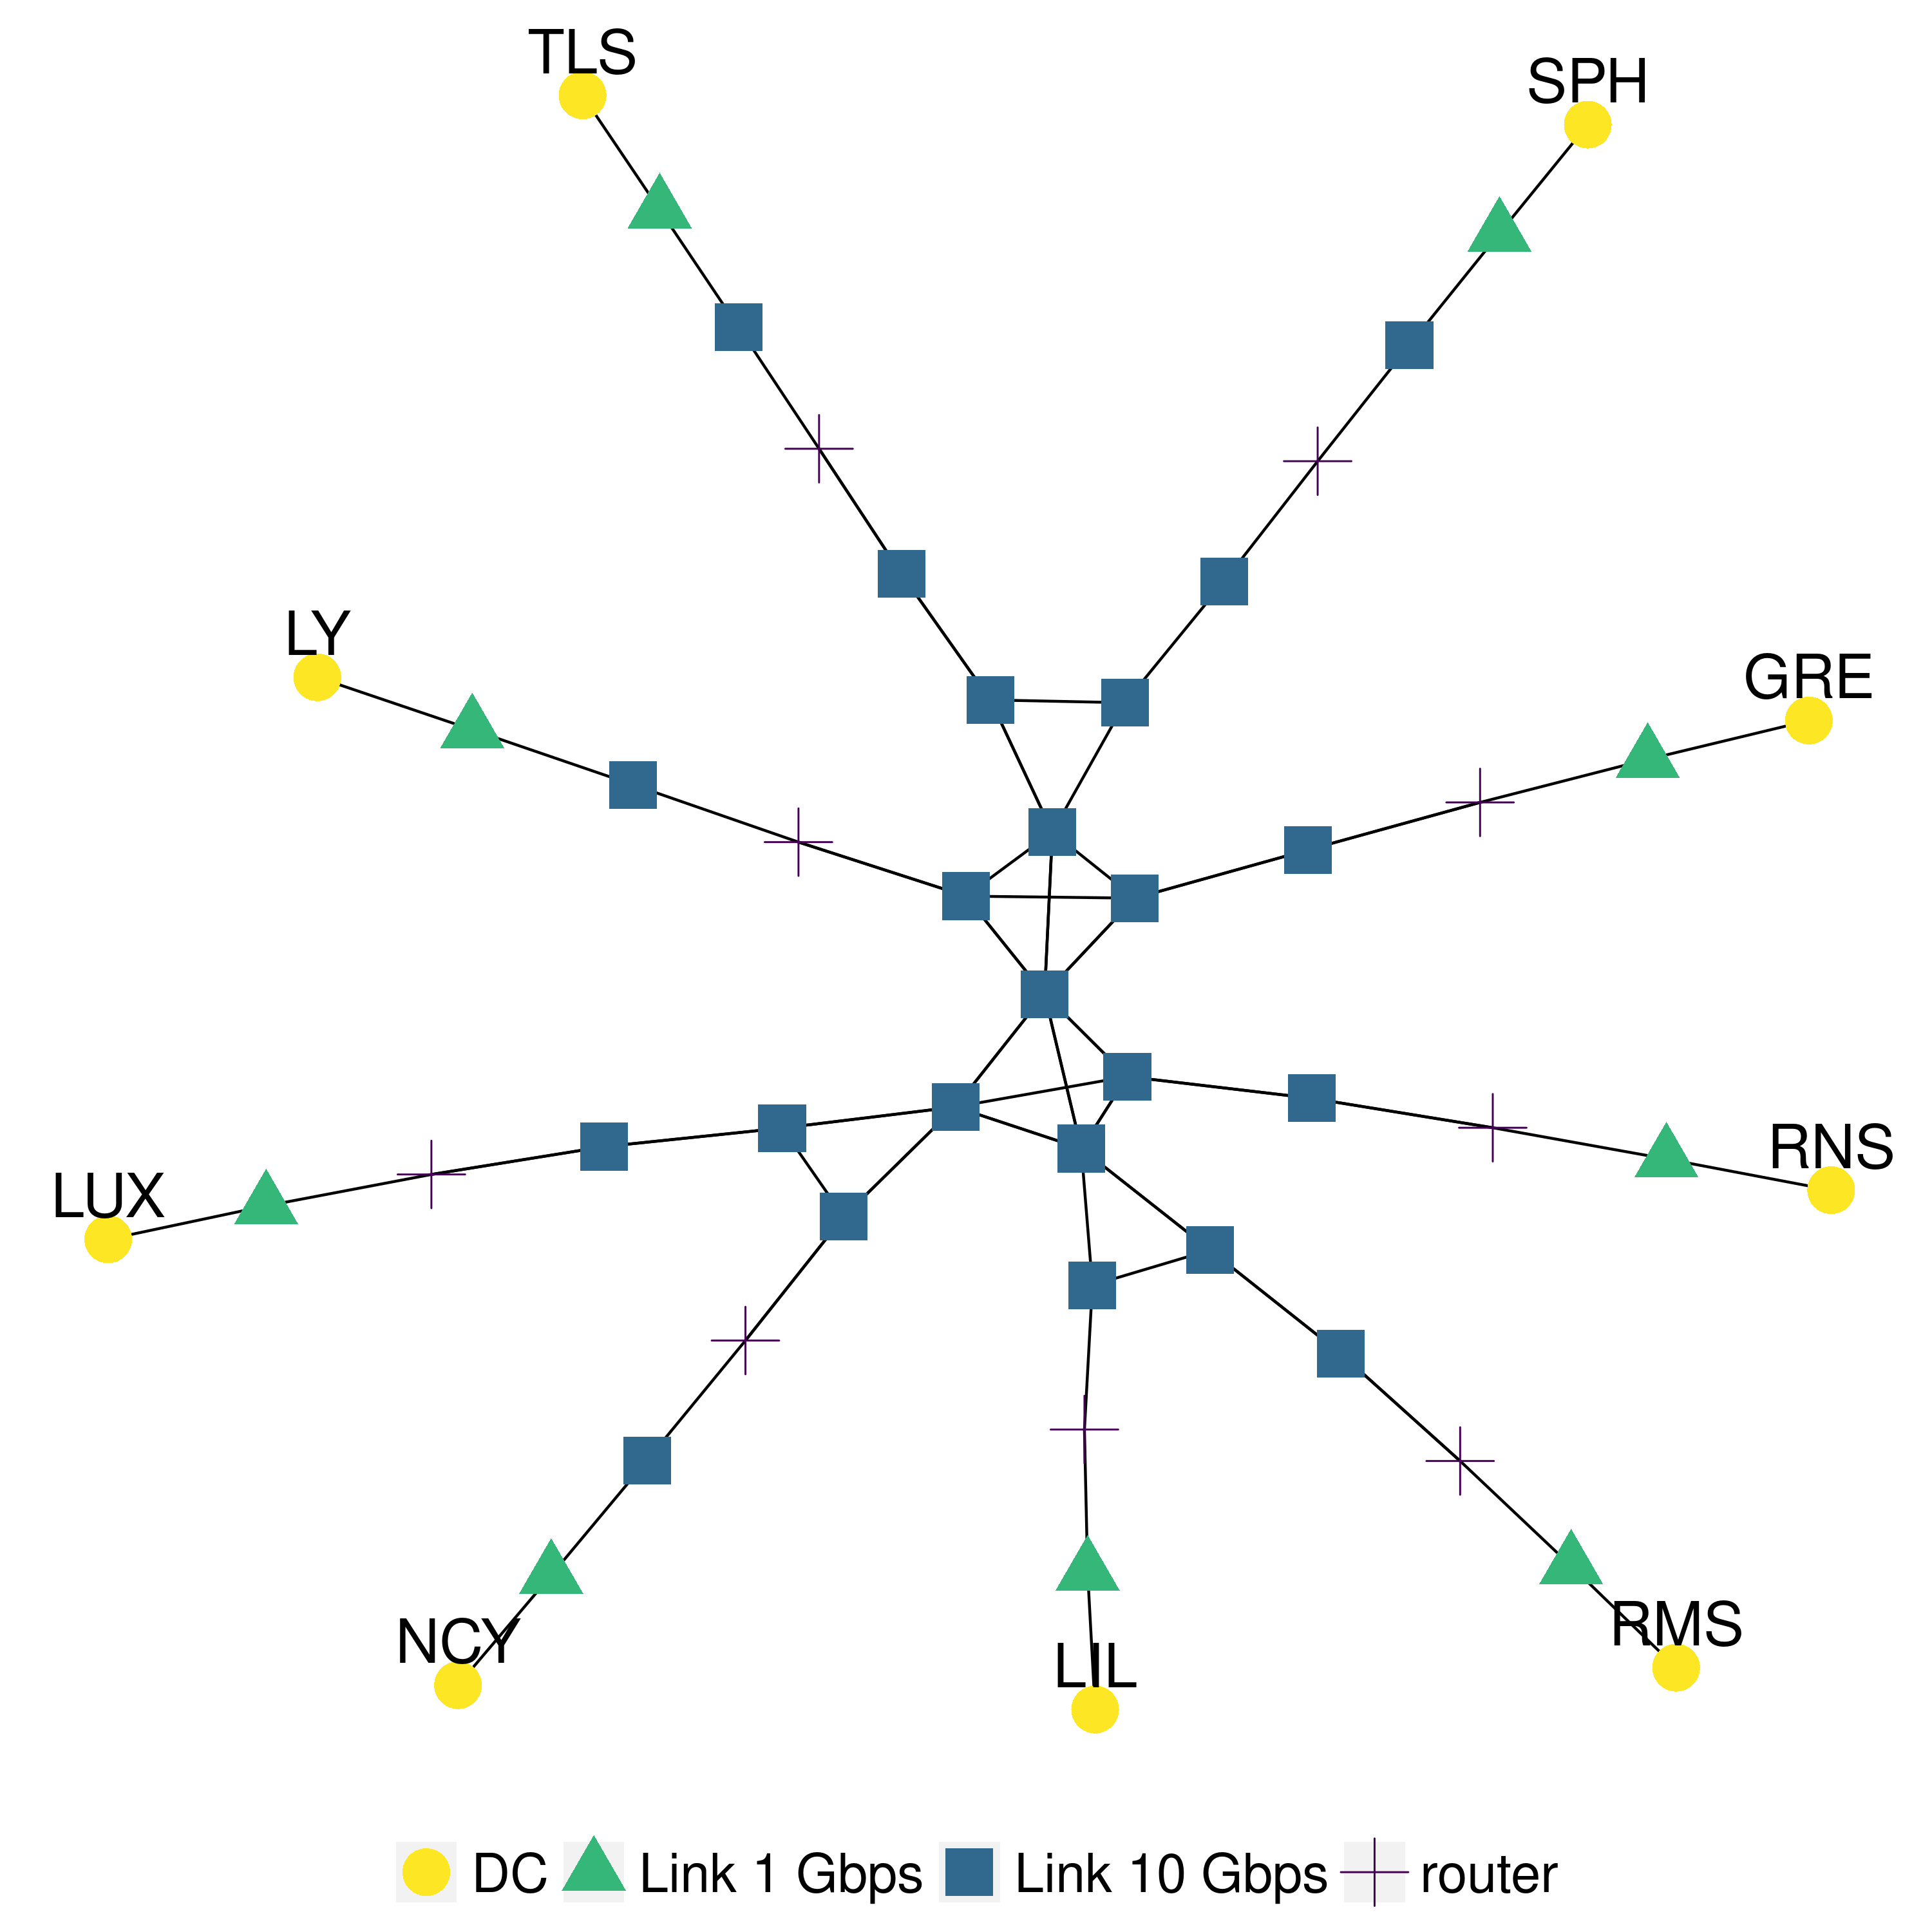
\epsfig{file = images/topology.PNG, width = .7\textwidth}}
  \caption{Topology of the Cloud platform, where ``GRE'' is Grenoble,  ``LIL'' is Lille, ``LUX'' is Luxembourg,``LY'' is Lyon, ``NCY'' is Nancy, ``RMS'' is Reims,  ``RNS'' is Rennes, ``SPH'' is Sophia, and  ``TLS'' is Toulouse.}
  \label{fig:topology}
 \end{figure}
 


Regarding the energy consumption of the servers, it is considered a linear model based on CPU usage, and the VMs always use 100\% of the requested number of CPU cores. The server presents a fixed consumption for its IDLE state (97~W), and the power consumption based on core usage is as follows: 128~W for 1 core; 146.4~W for 2 cores; 164.8~W for 3 cores; 183.2~W for 4 cores; 201.6~W for 5 cores; and 220~W with 6 cores. Furthermore, the energy consumption of turning on a server (127~W during 150 s), turning off a server (200 W for 10 s), and when the server is off (8 W) are modeled as well. Finally, only the power consumption of the servers is considered to model the power consumption of the DCs (Power Usage Effectiveness, or P.U.E., equals to 1), as we are focusing on the energy consumption of the computing part --- the major consumer. Choosing a P.U.E. different than 1 would not affect the scheduling decisions made by the migration planning algorithm, since only the total power consumption would be increased by a constant factor, and the ordering of the DCs in terms of green energy availability would be the same. Furthermore, we consider a homogeneous P.U.E for all the DCs, given that the DCs are inside the same country.


\subsection{VM live migration model}

The VM live migration model of NEMESIS has 3 phases. In the first phase, all the memory pages of the VM are transferred to the destination server. In the second, after completing the copy of all the memory pages, a message is sent to notify the end of the stop-and-copy step. Finally, in the last step, the commitment message is sent to the new host to inform the end of the migration process, and the VM will be destroyed in the server of origin and resumed in the destination host. 

The duration of the migration is essential information for the scheduling decision, as it can help avoid oversaturating the network links and generating network congestion. Algorithm~\ref{alg:estimation} is an extension of the NEMESIS algorithm, and it executes this estimation, where: \textit{linkLatency} is the latency of the link; \textit{routeSize} is the number of links that interconnects the host where the VM is originally running to the target host of the migration; \mbox{\textit{windowSize}} = 4,194,304 Bytes, is the TCP maximum window size; \textit{bandWidthRatio} = 0.97, represents the additional load caused by the headers of TCP/IP; \textit{bandwidth} = the minimum bandwidth among the links that interconnect the host of origin with the target host; $\alpha$ = 13.01, simulates the TCP slow start factor, that is, not all the bandwidth is instantly available for the communication; and $\gamma$ is used to represent the Bottleneck effect of the TCP protocol. The parameters used in Algorithm \ref{alg:estimation} were based on \cite{velho2013simgridparameters}. The difference between Algorithm \ref{alg:estimation}  and NEMESIS is the \textit{routeSize} variable: NEMESIS used fixed values (5 for live migrations intra-DC, and 11 for live migrations inter-DC), and now is assumed that the cloud operator has information about the network topology of his DCs, thus the real number of links that interconnect the two hosts is used.

\begin{algorithm}
\begin{algorithmic}
\caption{Estimation of the migration duration.}\label{alg:estimation}
\State $theLatency \gets linkLatency \cdot routeSize$
\State $transferLat \gets theLatency + \frac{\gamma}{bandwidth}$
\State $throughputL \gets \frac{windowSize}{2 \cdot transferLatency}$
\State $throughputB \gets bandwidth$
\State $throughput \gets min(throughputL, throughputB)$
\State $throughput \gets throughput 
\cdot bandWidthRatio$
\State $timeToMigrate \gets  3 \cdot \alpha \cdot transferLat + \frac{vmRamSize}{throughput}$ 
\end{algorithmic}
\end{algorithm}

\section{Planning the migrations}
\label{sec:modeling_smargreens}

Algorithms \ref{alg:general} and \ref{alg:detailed} plan the VM migrations considering the network topology and the bandwidth usage. They are inspired in the migration planning of NEMESIS, with the following modifications: i) the available bandwidth of the links is considered (it changes based on the number of migrations that use the same network link); ii) migrations can be performed in parallel between different DCs respecting the links bandwidth constraint; iii) the intra-DC migrations (for the server consolidation) are sequentially distributed in time (do not execute simultaneously) ; iv) the real number of links that interconnects the origin and the target server is used as input for the estimation algorithm of the migration duration. 

\begin{algorithm}
\begin{algorithmic}
\caption{General planning of the migrations.}\label{alg:general}

\State $DCs$ \Comment{Sorted by increasing ERGE}
\State $plannedTime \gets 0$
\State $timeSlotDuration \gets 300$
\State $linksHistory \gets \emptyset$
\While {$plannedTime < timeSlotDuration$}
\State $dc\_tx \gets $ first item of $DCs$  %\Comment{DC where the VM is initially running}
    \While {$dc\_tx \neq$ last item of $DCs$}
        \State $dc\_rx \gets $ last item of $DCs$
        \If{$dc\_tx$ has VMs that can be migrated}
            \While{$dc\_tx \neq dc\_rx$}
            \State evaluate if it is worth to migrate VMs from $dc\_tx$ to $dc\_rx$ using Alg. \ref{alg:detailed}
            \State $dc\_rx \gets$ previous DC of $DCs$
            \EndWhile
        \EndIf
        \State $dc\_tx \gets$ next DC of $DCs$
    \EndWhile
    \If{no VM migration was planed and no migration is in execution }
       \State \textbf{exit}
    \EndIf
    \State $plannedTime \gets$  instant after the expected end of next migration 
\EndWhile
\end{algorithmic}
\end{algorithm}


\begin{algorithm}
\begin{algorithmic}
\caption{Detailed migration planning between two DCs.}\label{alg:detailed}
\Require $dc\_tx,dc\_rx$

\State $VMs \gets$ list of VMs of $dc\_tx$
\For{$vm$ in $VMs$}
    \State $origin \gets$ server where the $vm$ is running
    \State $target \gets$ server from $dc\_rx$ being evaluated
    \State $worth \gets brownMig < brownNotMig $
    \State $e\_time \gets $ estimate the migration time using Alg. \ref{alg:estimation} 
    \State $band\_ok \gets$ links between $source$ and $target$ can receive the additional load of the migration
    \If{ $worth$ and $band\_ok$ }
    \State registers the planning of the migration and updates the link history   
    \EndIf
\EndFor

\end{algorithmic}
\end{algorithm}

The algorithms work as follows. Initially, the DCs are sorted by increasing order of expected remaining green energy (ERGE). The DC with the most available energy (initially at the beginning of the list) is denoted by M, and N is the DC with the least green energy (initially at the end of the list). The main idea of the algorithms is to migrate VMs from the DCs that are expected to use brown energy to the DCs that are expected to have green energy. The algorithm receives as input the information of the running VMs (grouped by the servers) of the DC M. The planning starts at the beginning of the time slot. For each VM that can be migrated, the algorithm tries to find a server in the destination DC N with the following restrictions: i) it has available computational resources to host the VM (CPU and memory); ii) the links that interconnect the server of origin (where the VM is running) and the target server can receive the additional load of the migration without violating their bandwidth constraint; iii) the VM migration finishes during the current time slot (if the destination server is off, the time to turn the server on is taken into account); and iv) performing the migration reduces the expected brown energy consumption. If all these restrictions are respected, the VM is planned to migrate, and the algorithm registers in the \textit{linkHistory} that the links that connect these two servers will be used until the instant when the VM migration is expected to finish in order to compute the available bandwidth of the network links. If there are still remaining VMs that could be migrated from DC M, the algorithm will try to migrate to the DC N-1, and so on, until all the VMs from DC M are planned to migrate, or all the DCs are processed. After finishing processing for the DC M, the algorithm repeats the same process for the DC M+1 until all the DCs are processed. 

After evaluating all the possible migrations for the instant at the beginning of the time slot, the algorithm will use the link usage history to obtain information about when there will be available links in terms of bandwidth, that is, at what instant of time \texttt{t} the next migration is expected to finish.  If there are still VMs that could be migrated, the migration planning algorithm will be executed again using the availability of the bandwidth at instant \textit{t}. Then, the process repeats until there are no more VMs to migrate or the evaluation time reaches the end of the time slot.

Regarding the server consolidation, there are two differences to the original NEMESIS algorithm: i) it will only be applied to the DCs that didn't have inter-DC migrations planned to avoid generating network congestion --- given that the intra-DC migrations could use the same network links as the inter-DC migrations planned in the previous step; and ii) the migrations are distributed in time using the estimation computed with Algorithm \ref{alg:estimation} to avoid overlapping them.

The new algorithm is called c-NEMESIS, where the ``c'' stands for congestion and its full name is ``Congestion and Network-aware Energy-efficient Management framework for distributEd cloudS Infrastructures with on-Site photovoltaic production'', an extension of the NEMESIS algorithm with modifications in the steps ``migration of the running VMs'' and  ``server consolidation''.


The computational complexity of the Algorithm \ref{alg:detailed} is $O(n_{VMS} \times  n_{servers} \times n_{links}  )$, where $n_{VMS}$ is the number of running VMs on the DC that is sending the VM, $n_{servers}$ is the number of candidate servers that have the least possible amount of free cores to run the VM in the destination host, and $n_{links}$ represents the number of links that interconnects the VM's host of origin and the target host. For Algorithm \ref{alg:general}, the computational complexity is given by $O(n_{DCs}\log{}n_{DCs} + {n_{DCs}}^{2} \times n_{VMS} \times  n_{servers} \times n_{links})$, where $n_{DCs}$ is the number of DCs.


\subsection{Energy cost of migrations}\label{sec:energy_costs_mig}

The energy consumption of a live VM migration is modeled in NEMESIS by a computation task that is executed in the target host. This task uses 100\% of a single CPU core during the migration process. Suppose the migration is impacted by network congestion. In that case, its duration will increase, resulting in a wastage of energy from the server where the VM was initially running as in the target server.


The wasted energy is proportional to the extra time migrating, that is, the difference between the duration of the migration process compared to the duration that it would take if there were no network congestion. A lower bound for the wasted energy can be computed with Algorithm \ref{alg:wasted_energy} using as input this extra time migrating. Given that the migration planning uses a ``follow-the-renewables'' approach to move the workload from the DCs that are using brown power at that instant to the DCs that have more available green energy, the algorithm computes individually the wasted energy in the server that is sending the VM and in the server that is receiving the VM. For the server that is sending the VM, this extra energy consumed is brown(er), increasing the overall brown energy consumption of the cloud, since this server could be turned off to save energy. For the server that will receive the VM, this extra energy is green(er), and it is wasted because it was only available at that instant of time (no energy storage devices) and could have been used to execute the workload.


\begin{algorithm}
\begin{algorithmic}
\caption{Extra energy consumption of migrating.}\label{alg:wasted_energy}

\State $pCore \gets 20.5$

\State $wastedOrigin \gets 0$
\State $wastedTarget \gets 0$

\For{$mig$ in $Migrations$}
    \State $vmCores \gets$ amount of cores of the VM being migrated
    \State $extraTime \gets mig.Time - mig.TimeNoCong$
    \If{$extraTime > 0$}
        \State $wastedOrigin += extraTime \cdot pCore \cdot vmCores$ 
        \State $wastedTarget += extraTime \cdot pCore$ 
    \EndIf
\EndFor
\end{algorithmic}
\end{algorithm}

The value of \textit{pCore} is an estimate for the additional cost of executing a core, and is obtained as follows: the server consumes \SI{220}{\watt} at full load and subtracting the power consumption of the IDLE state (\SI{97}{\watt}) it results in \SI{123}{\watt}. Finally, this value is divided by the total amount of cores of the server (6), resulting in \SI{20.5}{\watt}. Notice that \textit{pCore} is only multiplied by the number of cores of the VM for the server of origin, since it remains executing the VM until the end of the migration, and in the destination server the computational task uses only a single CPU core.


\section{Experiments}
\label{sec:simulations_smargreens}

The experiments were performed using computational simulations. The Simgrid \cite{CASANOVA20142899} (version 3.28) framework was used to develop the simulations because it allows modeling distributed computing experiments, such as cloud platforms, in particular: energy consumption of executing the tasks, turning on and off the servers, network usage by the live migration process, network topology and the network congestion. Another relevant reason for choosing the Simgrid framework is the fact that it is well-validated by the scientific community with over 20 years of usage. For the network, the default flow-level TCP modeling of Simgrid produces precise results for large distributed computing scenarios (as in our case with thousands of servers) in a reasonable amount of time. It is possible to use packet-level simulation, however, despite being more precise, it would result in huge execution time for the simulations \cite{velho2013simgridparameters}. Regarding the cloud infrastructure, it is considered the adapted version of the Grid'5000 (same as NEMESIS, see Section~\ref{sec:cloud_model}). Finally, it was simulated one week of the multi-cloud operation.

\subsection{Workload}

Traces from real cloud providers were used to generate the workload for the experiments. The data extracted from the traces were: the number of CPU cores requested, the instant of time when the task was submitted, and its duration. Regarding the requested RAM per VM, it is considered that each VM will consume 2 GB per core requested, similar to the \texttt{t2.small} instance of Amazon EC2\footnote{\url{https://aws.amazon.com/ec2/instance-types/}}. It is also considered that the VMs execute with a full CPU usage of the requested cores, the worst scenario for energy consumption. The workloads are scaled to use at a maximum of 80\% of the computational resources of the cloud platform at any given simulated time. This decision ensures that the tasks will always be allocated to the servers, and that there will be some room for the servers to receive VMs from live migrations, thus allowing analyzing the different scheduling approaches. Furthermore, from the cloud traces, it is possible to observe that the DCs are not used 100\% of their computational capacity. Figure \ref{fig:workload} illustrates the number of VMs submitted during the week (in yellow), and the cumulative demand of CPU cores requested at a given time (in purple), that is, the total number of CPU cores used by the VMs in execution at that instant of time. 

\begin{figure}[!htbp]
  \centering
   {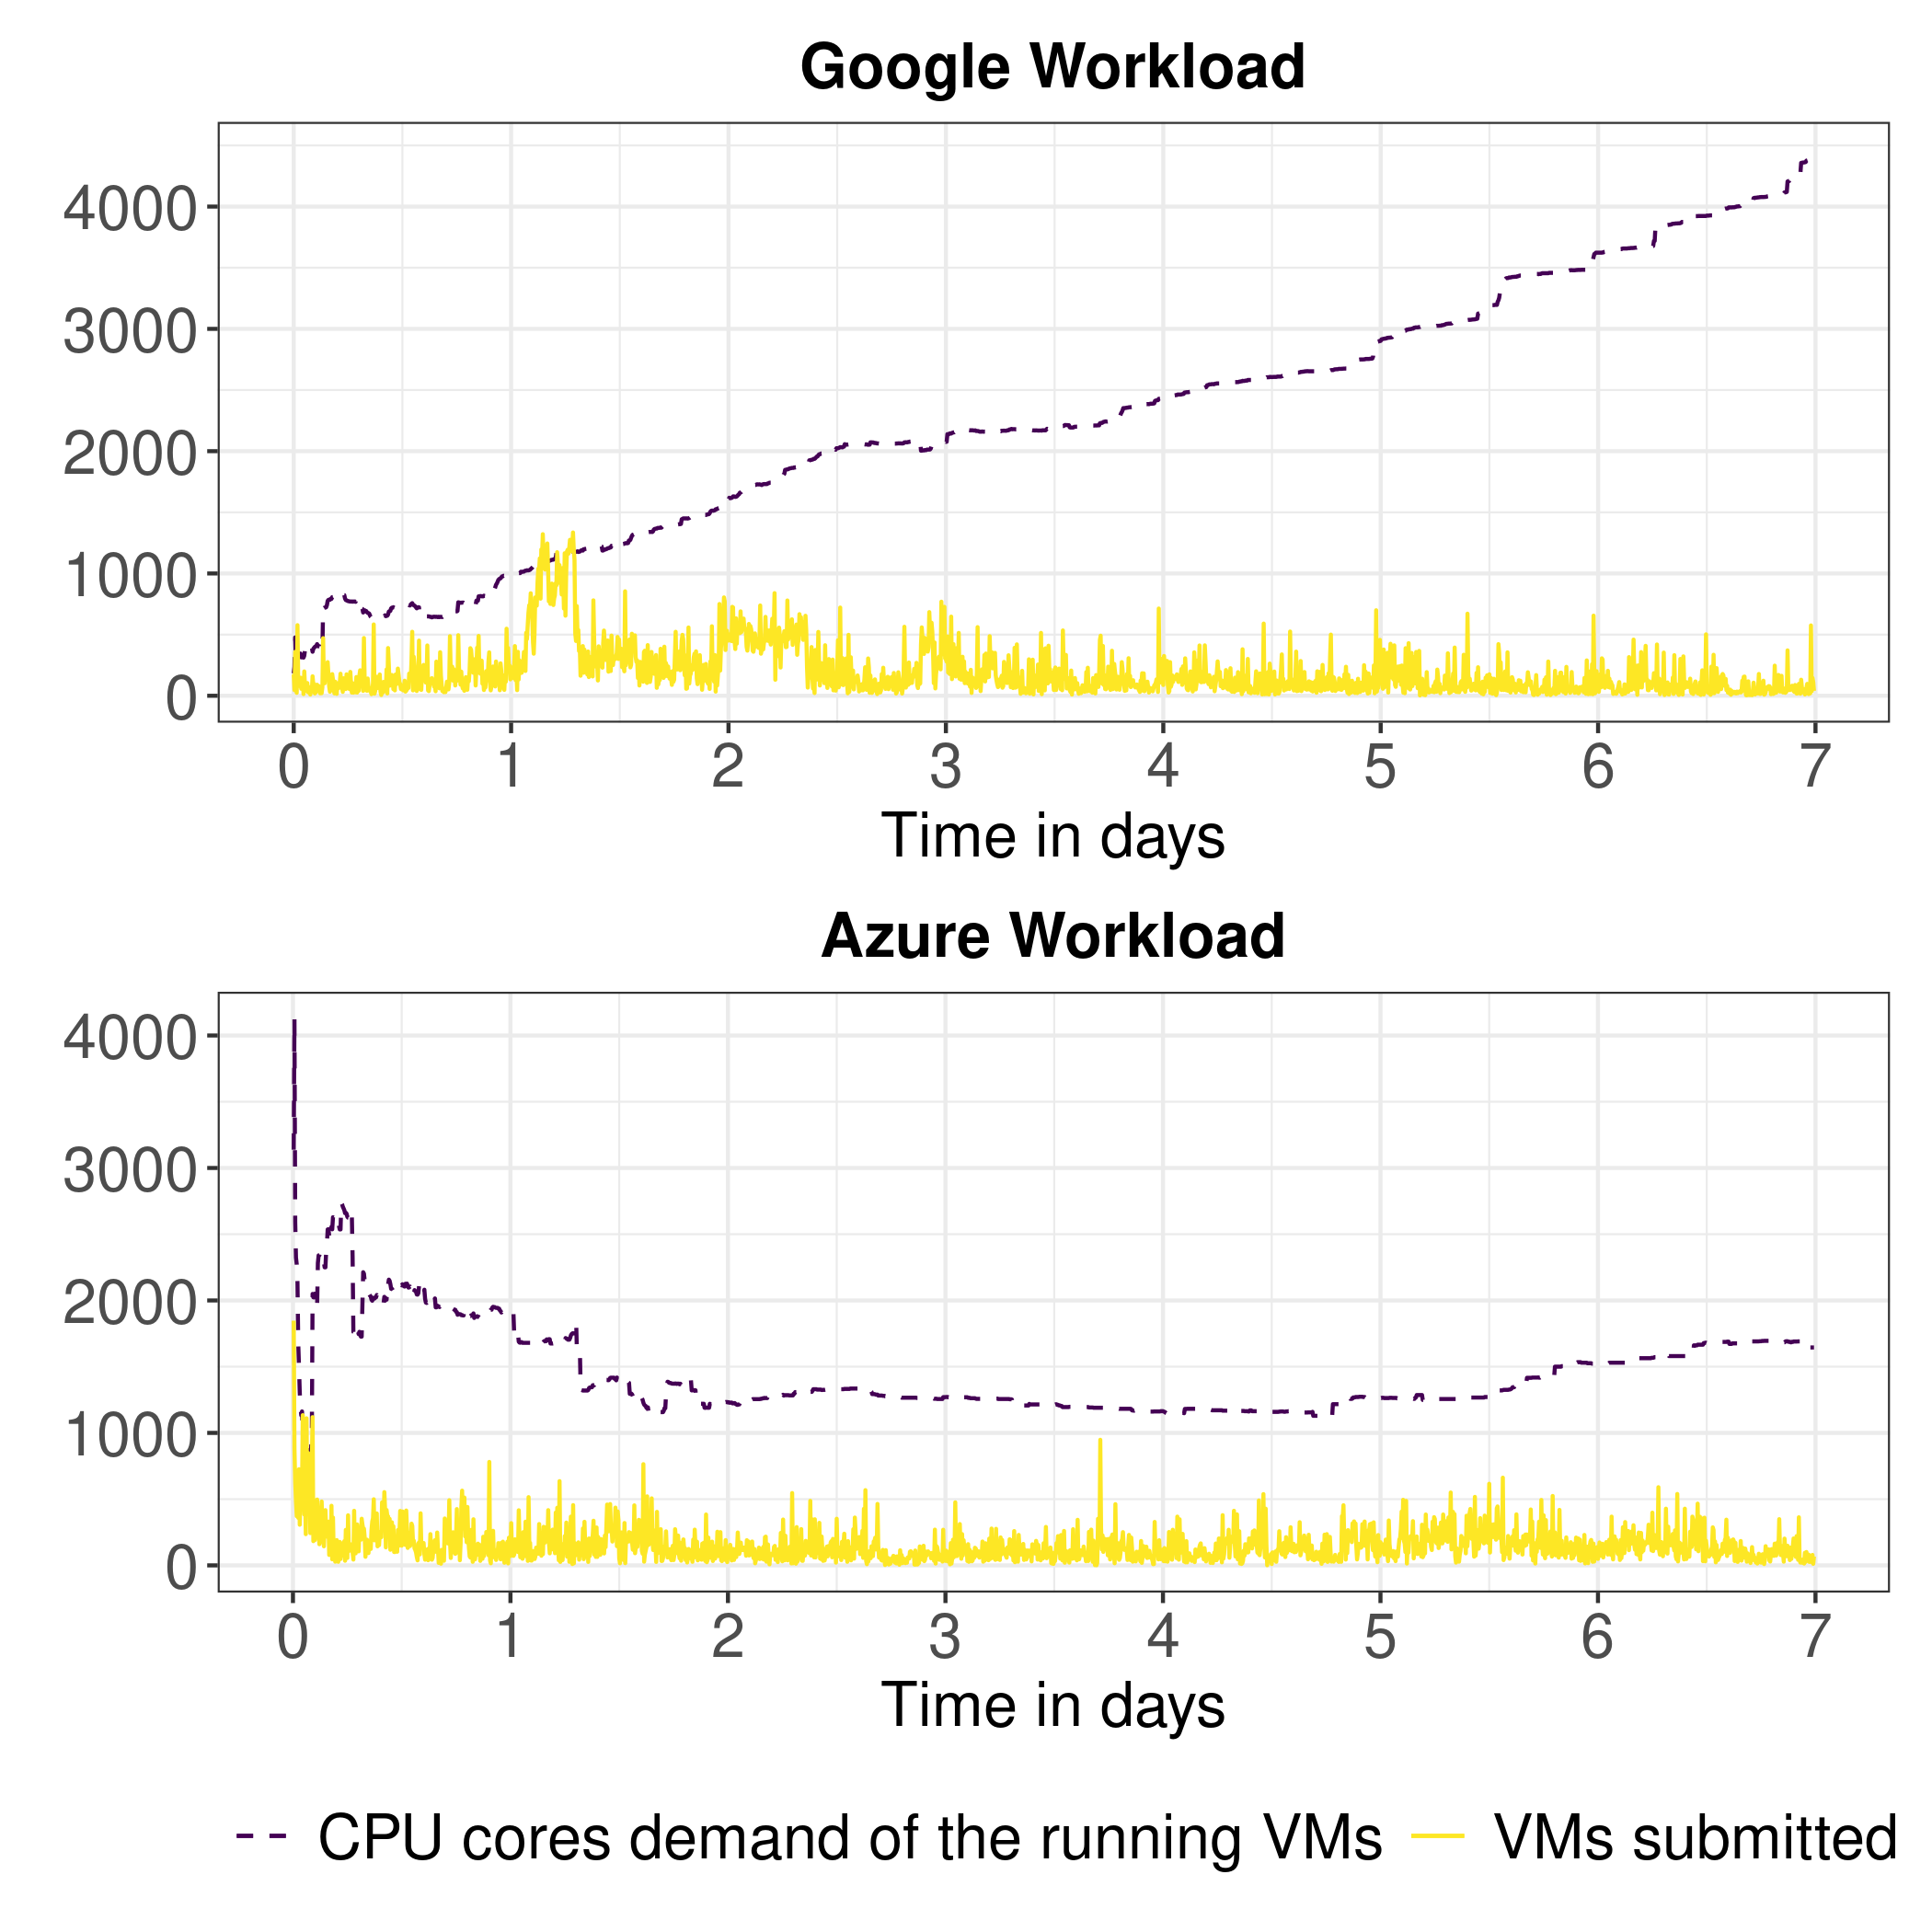
\epsfig{file = images/workloads.png, width = .6\textwidth}}
  \caption{Workloads used as input for our simulations.}
  \label{fig:workload}
 \end{figure}

The first workload was generated using as a base the 2011 Google Cluster Workload traces \cite{google2011traces}, and it consists of over 380,000 VMs. In this workload, the VMs have a long execution time, as can be seen in Figure \ref{fig:workload} that the value of the running VMs' CPU cores demand keeps increasing throughout the week. The second workload was based on traces from Microsoft Azure \cite{hadary2020protean}, more specifically, the Azure Trace for Packing 2020, and contains over 304,000 VMs. This generated workload has a different behavior than the previous one: there is a peak in the VM submissions at the beginning of the week, and the VMs have a shorter execution time, as seen that the CPU core demand does not keep increasing during the week.

These traces do not provide data about the network usage of the tasks and it was not modeled in the simulations. The additional load in the network is generated only by the live migration of the VMs. Therefore, this work can be seen as a lower bound for the real world scenario. 

\subsection{Green energy traces}

The data for the energy produced by the solar panels were obtained from the Photovolta\footnote{http://photovolta.univ-nantes.fr/} project by \textit{Université de Nantes}. The data represents the power production of two arrays of 4 PVs each (Sanio HIP-240-HDE4) with a total nominal power production of 1920 Wc at intervals of 5 minutes. In order to simulate the different production of the geographically distributed DCs,  a different week of the production trace was used for each DC. Furthermore, each DC had 3 PV panels per server. The PVs installed in the DCs generated the following amount of energy during the simulated week: i) Grenoble: 1.58 MWh; ii) Lille: 0.07 MWh; iii) Luxembourg: 0.15 MWh; iv) Lyon: 1.19 MWh; v) Nancy: 2.16 MWh; vi) Reims: 0.38 MWh; vii) Rennes: 1.63 MWh; viii) Sophia: 1.75 MWh; and ix) Toulouse: 1.53 MWh. In total, around 10.5 MWh of green power was produced in the simulated week. Figure \ref{fig:green_power} shows the green power production per DC during the simulated week.

 \begin{figure}[!htbp]
  \centering
   {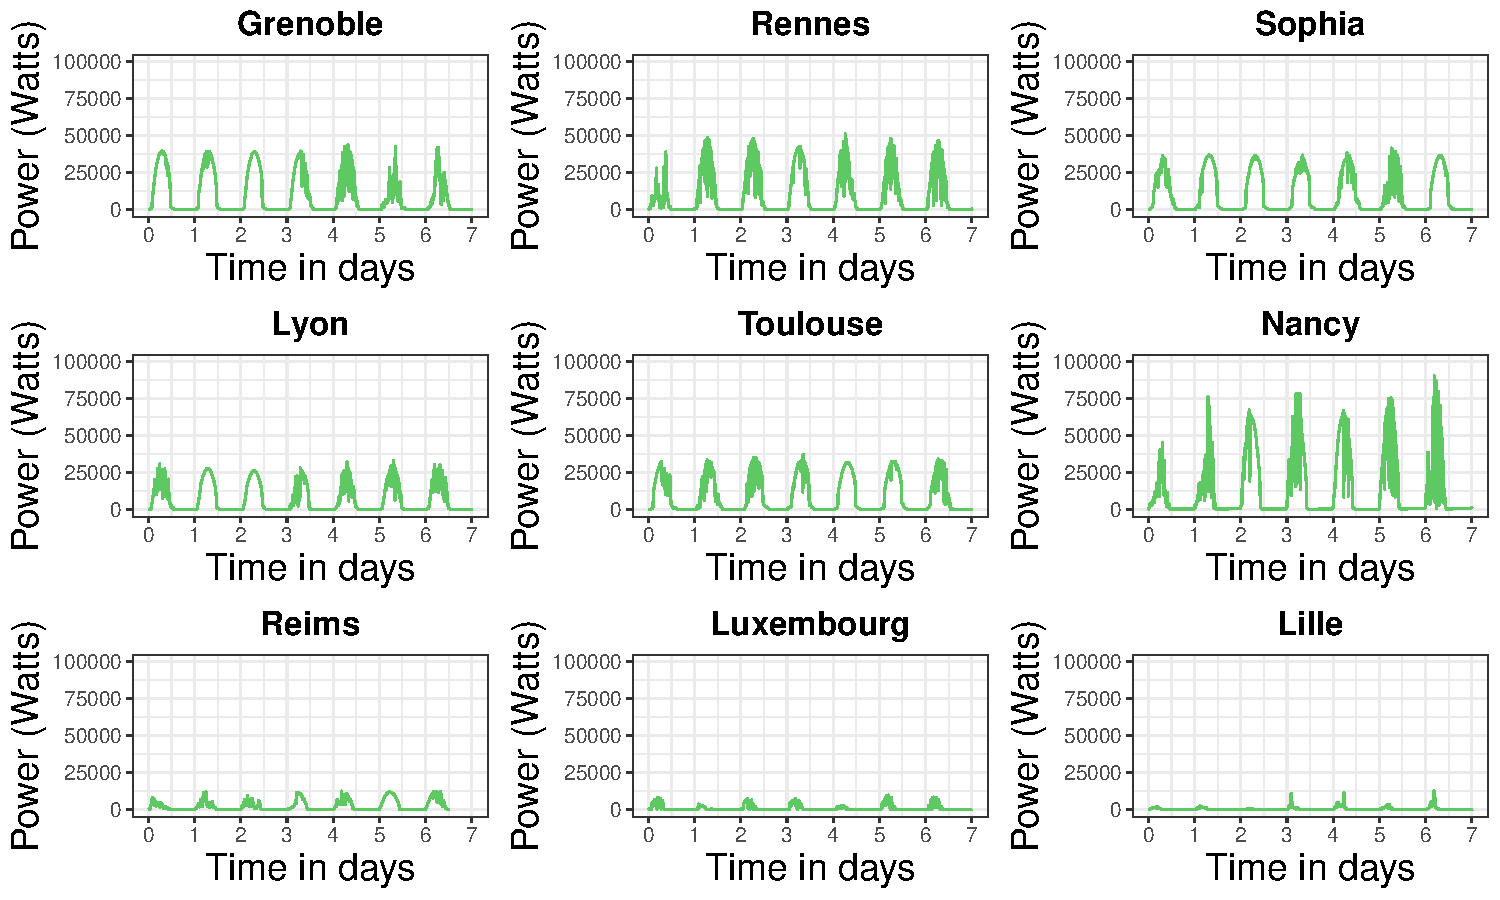
\epsfig{file = images/pv_pow_photovolta.pdf, width = \textwidth}}
  \caption{Green power production (in Watts) produced by DC during the
  simulated week.}
  \label{fig:green_power}
\end{figure}



\section{Results}

\label{sec:results_smargreens}

In this section,  the results of the simulations are presented. First, it is shown an analysis of the accuracy of an essential component of NEMESIS and c-NEMESIS algorithms: the algorithm for the duration of migration (Algorithm \ref{alg:estimation}. Then,  it is presented an analysis of the live migrations performed and their impact on network congestion, wasted energy, and the total and brown energy consumption. To further evaluate the effectiveness of using ``follow-the-renewables approaches'', results from two other state-of-the-art works (at the time the article was written, november of 2021) are presented that incorporate this approach in different ways.


The first is the Workload shifting non brownout (WSNB) algorithm \cite{XU2020191}. The algorithm works as follows. Initially, the VM is allocated to the nearest DC (aiming to reduce the response time) and to the server that will increase the energy consumption by the least (a server that is already on and its available computational resources are equal to or slightly greater than the requirements of the requested VM). Then, suppose this initial DC does not have available renewable power to execute the VM. In that case, the algorithm will evaluate another DC (the DCs are sorted by available green energy) that matches this demand and does not exceed a threshold for the response time. If another DC is found, the VM will be reallocated to it. The algorithm does not perform server consolidation with live migrations, it tries to use the minimum number of servers during this allocation. To adapt this baseline for the experiments, the response time restriction was removed from the algorithm, that is, we consider that all the DCs are homogeneous in terms of latency for the VM request, since the used workloads do not have this data, and this modification does not change the behavior of the algorithm.

The second work from state of the art is the FollowMe@Source (or FollowMe@S) algorithm \cite{ALI2021110907} that has two variants: i) FollowMe@S Intra, that only perform VM migrations inside the same DC (intra-DC migrations);  and ii) FollowMe@S Inter, that only perform VM migrations between different DCs (inter-DC migrations). Both algorithms have the same general steps, described as follows.


The FollowMe@S algorithm has two main steps: allocation and migrations. The allocation step begins by sorting the DCs by the availability of green energy. Then, the algorithm will search for a server that can host the VM, respecting the sorted list of DCs. If no server was found after searching through all DCs, the VM will be processed in the next scheduling round. The process will be executed again for all the other VMs to be scheduled. In the migration step, either only intra-DC or inter-DC migrations are performed. First, the algorithm obtains the list of all the VMs that are in execution at that instant of time. Then, it evaluates the usage of the servers to obtain the underutilized hosts (less than 20\% of CPU usage) and marks them to be turned off. The running VMs of these underutilized hosts will be removed using live migrations in order to turn them off and save energy. In the intra-DC case (FollowMe@S Intra), the algorithm will run in each DC separately. For each VM, it will try to find a server with available computational resources to host it, and the migration is performed if a server is found. In the inter-DC case (FollowMe@S Inter), for each VM that can be migrated, the algorithm will evaluate the DCs sorted by the availability of green energy, and migrate the VM to the server of the first DC that can host the VM. One important point to notice is that FollowMe@S does not consider the network to schedule its migrations. The following modifications were performed in the algorithm to adapt it for the experiments: i) it is not considered the network costs of a distributed algorithm, since NEMESIS, c-NEMESIS, and WSNB are centralized algorithms; ii) the workload degradation performance by migrating the VM --- for example migrating to a server with a less efficient CPU ---  is not modeled as a homogeneous platform is used.

The baselines adopt the ``follow-the-renewables'' approaches in different ways. The algorithms WSNB and FollowMe@S Intra only use ``follow-the-renewables'' for the initial scheduling, and the VMs are not migrated to other DCs during their execution. On the other hand, the algorithm FollowMe@S Inter performs VM migrations to other DCs --- the same strategy adopted by NEMESIS and c-NEMESIS.


A public Git repository hosts all the simulation code, the traces for the workloads and green power production, and the instructions to run and extract the results\footnote{https://gitlab.com/migvasc/c-nemesis}. Finally, the results from the experiments using these algorithms and workloads are deterministic. Therefore, only results for a single execution of the simulations are presented.


 \subsection{Accuracy of the estimation algorithm}
 
We define an underestimated migration as a VM live migration process with a longer duration than estimated. Table \ref{tab:migs_under} presents the number of live migrations that were underestimated by NEMESIS and c-NEMESIS, and the percentage value that is based on the total number of migrations (that can be found in Table \ref{tab:amount_migs}). For both workloads, c-NEMESIS presented almost no underestimation for the migrations compared to NEMESIS. Furthermore, it is interesting to notice that virtually all the intra-DC migrations were underestimated in NEMESIS because they start simultaneously, resulting in network congestion.

\begin{table}[!ht]
\caption{Number of underestimated live migrations and the ratio of the overestimation, where ``W'' stands for ``Workload'', ``G'' for Google, and ``A'' for Azure.}\label{tab:migs_under} \centering
\begin{tabular}{|l|c|r|r|}
  \hline
  \textbf{Algorithm} & \textbf{W}  & \textbf{Inter} & \textbf{Intra}   \\
  \hline
  NEMESIS  & G & 245 (4.4\%)   & 3 393 (95.7\%) \\
  \hline
  c-NEMESIS & G & 0 (0\%)  & 61 (2.9\%) \\
  \hline
  NEMESIS & A & 140 (3.6\%)   &  3 324 (94.1\%)   \\
  \hline
  c-NEMESIS & A & 24 (0.1\%)   & 49 (3.8\%) \\
  \hline  
\end{tabular}
\end{table}


In order to evaluate the estimation algorithm for the duration of the migrations, two metrics are used to assess its accuracy: the Mean Absolute Percentage Error (M.A.P.E.) and the Root Mean Square Error (R.M.S.E.). The M.A.P.E. is defined by: $ \frac{1}{n}\sum_{i=1}^{n}  \frac{| R_{i} - F_{i}|}{R_{i}}$, where $n$ represents the amount of values being considered, $i$ the index of the value being considered, $R_{i}$ the real duration of migration, and $F_{i}$ the estimated duration. The results of the M.A.P.E. is a percentage value, and it represents the relative value of the estimation errors compared to the original value, thus it is an easy-to-understand metric. The R.M.S.E. is defined by: $\sqrt{ \frac{1}{n}\sum_{i=1}^{n}  (R_{i} - F_{i})^2}$. The R.M.S.E. is a metric similar to the standard deviation, and it allows us to validate how far the estimation was from the original value.


\begin{table}[!htpb]
  \caption{Accuracy measurements, where ``W'' stands for ``Workload'', ``G'' for Google, and ``A'' for Azure. The M.A.P.E. value is in percentage (\%), and the R.M.S.E. in seconds. }\label{tab:accuracy} \centering
\begin{tabular}{|l|c|r|r|}
  \hline
  \textbf{Algorithm} & \textbf{W}  & \textbf{M.A.P.E.} & \textbf{R.M.S.E.}\\
  \hline
  c-NEMESIS  & G & 0.70  & 0.395 \\
  \hline
  NEMESIS & G & 32.895 & 18.56 \\
  \hline
  c-NEMESIS  & A & 0.649  & 0.432 \\
  \hline
  NEMESIS & A & 34.01 & 20.03 \\
  \hline
\end{tabular}
\end{table}



Table \ref{tab:accuracy} presents the results for the accuracy measurements. It is possible to observe that c-NEMESIS is accurate with low error values. Two points justify the improvement in the precision of the estimation algorithm: i) the new algorithm has full information on the network topology and uses the actual number of links that interconnect the servers involved in the migration process; ii) since it is more precise, the migration planning results in less network congestion, which affects the duration of the migration.


\subsection{Analysis of the VM live migrations performed}


Table \ref{tab:amount_migs} presents the number of live migrations performed during the simulated week. NEMESIS performed the lowest number of inter-DC migrations for both workloads, since its migration planning does not allow for migrations in parallel leaving or arriving at the same DC. The c-NEMESIS algorithm executed more inter-DC migrations than NEMESIS, as it takes into account the network topology and allows for migrations in parallel. c-NEMESIS had the lowest number of intra-DC migrations for two factors: i) the server consolidation step is only executed for the DCs that do not have inter-DC migrations planned in a time slot; and ii) intra-DC migrations are distributed in time. The FollowME@S algorithm had the highest number of inter and intra-DC migrations because the planning does not consider network usage.

\begin{table}[!ht]
\caption{Number of VM live migrations performed, where ``W'' stands for ``Workload'', ``G'' for Google, and ``A'' for Azure. }\label{tab:amount_migs} \centering
\begin{tabular}{|l|c|r|r|}
  \hline
  \textbf{Algorithm} & \textbf{W}  & \textbf{Inter} & \textbf{Intra}   \\
  \hline
  NEMESIS  & G & 5 617  & 3 545 \\
  \hline
  c-NEMESIS & G & 18 056  & 2 074 \\
  \hline
  FollowMe@S Intra  & G & 0  & 560 862 \\
  \hline
  FollowMe@S Inter  & G & 96 464 & 0 \\
  \hline
  NEMESIS & A & 3 863 & 3 532 \\
  \hline
  c-NEMESIS & A & 17 479  & 1 300 \\
  \hline
  FollowMe@S Intra  & A & 0  & 177 086 \\
  \hline
  FollowMe@S Inter   & A & 93 388 & 0 \\
  \hline
\end{tabular}
\end{table}

\subsubsection{Total and brown energy consumption of the cloud platform}

Table \ref{tab:total_energy_cons} presents the cloud platform's total and brown energy consumption for the simulated week. The c-NEMESIS performed better in terms of brown energy usage, having the lowest consumption among the other evaluated algorithms --- except for NEMESIS using the Azure workload, in which the consumption was the same. Regarding the total energy, c-NEMESIS consumed more than NEMESIS because it performed more migrations. On the other hand, more green energy was harnessed, since the brown energy consumed was the same or lower. Regarding the FollowME@S algorithm, both inter and intra versions had similar brown energy consumption, but the inter-DC approach had a marginally lower brown energy consumption than the intra-DC (around 0.3\% for the Google workload and 0.04\% for the Azure workload). The WSNB algorithm had the highest consumption of both total and brown energy.

\begin{table}[!h]
\caption{Comparison of energy consumption (MWh), where ``W'' stands for ``Workload'', ``G'' for Google, and ``A'' for Azure.}\label{tab:total_energy_cons} \centering
\begin{tabular}{|l|c|r|r|}
  \hline
  \textbf{Algorithm} & \textbf{W} & \textbf{Total} &  \textbf{Brown} \\
  \hline  
  NEMESIS  & G & 25.46 & 17.23 \\
  \hline
  c-NEMESIS & G & 25.56 & 17.18 \\
  \hline
  FollowMe@S Intra  & G & 27.56 & 19.13 \\
  \hline
  FollowMe@S Inter  & G & 27.59 & 19.07 \\
  \hline
  WSNB  & G & 29.49 & 20.89 \\
  \hline
  NEMESIS  & A  & 30.43 & 21.21 \\
  \hline
  c-NEMESIS & A  & 30.55 & 21.20 \\
  \hline
  FollowMe@S Intra  & A  & 31.69 & 22.41 \\
  \hline
  FollowMe@S Inter  & A  & 31.69 & 22.40 \\
  \hline
  WSNB & A   & 33.56 & 24.23 \\
  \hline
\end{tabular}
\end{table}

The difference between the total and brown energy consumed with the green energy generated in the simulated week (10.5 MWh) is compared to obtain the green energy usage of the algorithms. For the Google workload, the usage of green energy was: c-NEMESIS = 80\%, NEMESIS = 79\%, FollowMe@S Intra = 80\%, FollowMe@S Inter = 81\%, and WSNB = 82\%. Regarding the Azure workload, the usage was: c-NEMESIS = 89\%, NEMESIS = 88\%, FollowMe@S Intra = 89\%, FollowMe@S Inter = 89\%, and WSNB = 89\%. 


The scheduling policies and how the algorithms adopt the ``follow-the-renewables'' strategy justify the difference between the total and brown energy consumption, and the relative value of renewable energy used. The algorithms WSNB and FollowMe@S Intra that presented the highest brown energy consumption applied ``follow-the-renewables'' at the initial scheduling of the workload, and didn't migrate the VMs in execution to other DCs as the green energy availability changed over time --- as did by the algorithms FollowMe@S Inter, NEMESIS and c-NEMESIS. The next section analyses the live migrations' impact on total and brown energy consumption to further understand the difference in these results.

\subsubsection{Wasted resources in the migrations}
\label{sec:wasted_resources_smartgreens}
To evaluate the wastage of resources in terms of network and energy, all the live migrations performed in the algorithms are compared with a perfect scenario: all the migrations are performed individually and isolated, having full access to the network.

Table \ref{ tab:wasted_seconds } presents statistics about the extra time (in seconds) it took to migrate the VMs in the simulations in comparison with the perfect scenario. The absolute value is the absolute difference in seconds. For example, on average, the live migrations performed by the NEMESIS algorithm were 10.11 seconds longer compared to the perfect scenario for the Google workload. The relative value is the ratio of the difference. For example, in the FollowMe@S Inter with the Google workload, the migration duration was more than 10 times longer in comparison with the perfect scenario.


\begin{table*}[!ht]
  \small

\caption{Extra seconds during migrations compared to the case when there is no congestion, where ``W'' stands for ``Workload'', ``G'' for Google and, ``A'' for Azure. ``avg.'' for the average of the observations, ``max.'' for the maximum value, ``abs.'' for the absolute value, and ``rel.'' for the relative value.} \label{ tab:wasted_seconds } \centering
\begin{tabular}{|l|c|r|r|r|r|r|}
  \hline  
  \textbf{Algorithm} & \textbf{W}  & \textbf{avg. abs.} &  \textbf{max. abs.} & \textbf{avg. rel.} &  \textbf{max. rel.} &  \textbf{Total sec.} \\
  
  \hline
  NEMESIS  & G & 10.11  & 56.98 & 1.53 & 3.98  & 92 915\\
  \hline
  c-NEMESIS & G & 0.22  & 0.88 & 1.0 & 1.05  & 4 331 \\
  \hline
  FollowMe@S Intra & G & 113.94  & 1 028.51 &  6.37  & 40.82  & 64 525 098 \\
  \hline
  FollowMe@S Inter & G & 215.18  & 4 875.8 & 10.67 & 155.5  & 22 058 949\\
  \hline
  NEMESIS  & A & 11.62  & 62.96 & 1.59 & 3.98  & 86 235 \\
  \hline
  c-NEMESIS & A &  0.23 & 6.14   & 1.0 & 1.32  & 4 224\\
  \hline
  FollowMe@S Intra & A & 91.08  & 938.48 & 4.39 & 25.56  & 16 384 188  \\
  \hline
  FollowMe@S Inter & A & 186.56  & 8 047.89 & 7.8 & 157.24  & 18 531 893 \\
  \hline

\end{tabular}

\end{table*}

The c-NEMESIS algorithm had the best performance in terms of extra seconds spent migrating for both workloads, with values close to the perfect scenario: the average relative difference (avg. rel.) was approximately 1. The NEMESIS algorithm had a good performance as well with low extra seconds values, and the duration of the migrations took, on average, about 1.5 more than in the perfect scenario. The migrations performed by FollowME@S, both intra and inter-DC cases, had the worst performance: the duration took, on average, from 4 to 10 times more than the perfect scenario. These results highlight the importance of considering the network for the migration scheduling, since c-NEMESIS and NEMESIS presented the lowest wastage of resources.
                      

Using the extra seconds spent in the migrations, a lower bound for the wasted energy is computed using Algorithm \ref{alg:wasted_energy} for both the servers that sent the VM (origin) --- that represents the brown(er) energy consumption --- and the servers that received the VMs (target) --- that represents the green(er) energy waste. Table \ref{tab:wasted_mig} presents the results. The algorithm FollowMe@S (both inter and intra-DC versions) was the algorithm that wasted the most energy. The c-NEMESIS algorithm had the lowest wastage of energy overall, despite performing more migrations than NEMESIS (the second best in wastage of energy). These values are justified by the fact that wasted energy is directly proportional to the duration of the migrations, thus bad planning will congest the network and, as consequence, increase the total energy consumption. Finally, it is important to notice that the green wasted energy is not negligible and can be used to power the cloud. For example, in the FollowMe@S intra-DC with the Google workload, the wasted green energy could have powered the Luxembourg DC for approximately 44 hours (at 100\% computational performance).



\begin{table}[!ht]

\caption{Wasted energy in the migrations (Wh) in comparison to the perfect scenario where the migration process have full access to the network links. In the table ``W'' stands for ``Workload'', ``G'' for Google, and ``A'' for Azure.}\label{tab:wasted_mig} \centering
\begin{tabular}{|l|c|r|r|}
  \hline
  \textbf{Algorithm} & \textbf{W}  & \textbf{Origin} & \textbf{Target}   \\
  \hline
  NEMESIS  & G & 545.1  & 529.1 \\
  \hline
  c-NEMESIS & G & 35.42  & 24.67 \\
  \hline
  FollowMe@S Intra & G & 473 971.6 & 367 434.6 \\
  \hline
  FollowMe@S Inter & G & 153 829.96  & 125 613.5  \\
  \hline
  NEMESIS  & A & 539.59  & 491.06 \\
  \hline
  c-NEMESIS & A &  39.31 & 24.06   \\
  \hline
  FollowMe@S Intra & A & 163 128.14  & 93 298.9  \\
  \hline
  FollowMe@S Inter & A & 175 086.3  & 105 528.8 \\
  \hline

\end{tabular}
\end{table}


\section{Summary} \label{sec:conclusion_smargreens}


Reducing the environmental impact of the operation of cloud computing platforms, particularly the carbon footprint generated from the country-like the energy consumption, is a complex and challenging problem currently being addressed from multiple angles. In this chapter, we focus on the strategy ``follow-the-renewables'' and study the indirect impact on the energy consumption caused by the additional load generated in the network. The experiments were based on real-world data for the cloud infrastructure, workloads, and photovoltaic power production.

This chapter demonstrates that the indirect network impact on the energy consumption in multi-clouds for ``follow-the-renewables'' approaches is generated by bad scheduling policies for the migrations, which results in network congestion --- as the live migrations compete for the available bandwidth of the network links, affecting not only the applications that are running inside the VMs, but as well the duration of the migration process. Given that migrating a VM also consumes energy --- proportional to its duration --- and that the workload will be sent to the DCs using green(er) energy (``folllow-the-renewables''), the extra energy consumption is in reality wasted energy that could be used to power the cloud platform. Furthermore, the adoption of the ``follow-the-renewables'' needs to consider the whole execution of the workload:  the state-of-the-art algorithms that only used the green energy information for the initial scheduling and didn't migrate the workload as the availability of renewable energy changed had the highest brown energy consumption. 

The proposed estimation algorithm for the duration of the live migrations that uses as input information about the communication network of the data centers (network links latency, bandwidth and topology) is accurate. By using this estimation algorithm and using as input the network characteristics of the cloud, the migration planning of c-NEMESIS was able to increase the number of migrations by at least 3-fold without network congestion, while maintaining or reducing the brown energy consumption in comparison to other state-of-the-art works.

As future research directions, the network usage by the workload and how it will compete for network resources with the live migrations needs further investigation. It is also possible to extend the proposed solutions for other virtualization techniques as containers by updating the estimation algorithm with a model for container live migration. Finally, some approaches explore turning off the network devices to save energy. This technique reduces the available network links in the cloud platform, and the network traffic will be re-routed, and it is necessary to analyze if the energy savings are more significant than the impacts caused by the network congestion.


%=========================================================================================

%============================================================================================================


\chapter[Sizing the renewable infrastructure to greener the DC operation]{Sizing the renewable infrastructure to greener the DC operation\footnotemark}
\label{chap:ccgrid}

\section{Introduction}

%In order to reduce the environmental impact of data centers' operation, major cloud players committed to include renewable energy in their operation, such as Google, Apple, Microsoft, Amazon AWS, and Facebook \cite{Greenpeace2017}. \mv{Furthermore, solar energy costs have fallen 85\% (and are expected to keep decreasing) and its deployment increased over than 10 times from 2010 to 2019 \cite{ipcc2022_data_pv}. Moreover, the solar irradiation has a lower variation than wind speed \cite{krakauer2017prediction_accuracy}, which can increase the accuracy of predictions for the workload scheduling decision.} 

On the previous chapter, we saw the adoption of the carbon-aware technique follow-the-renewables applied to a multi-cloud distributed over a country, and the drawbacks it presents if not used properly, as network congestion and extra energy consumption. Now, the reader will be presented to another strategy: sizing (or dimensioning) the renewable infrastructure to reduce the carbon footprint of the cloud operation. This strategy consists in defining how much investments needs to be made, for example defining the area of solar panels (when considering solar power), the number of wind turbines, and the capacity of the energy storage devices (as lithium-ion batteries) that needs to be manufactured. 

The scenario considered has some differences to better represent modern cloud providers. First, it is considered that the DCs are geographically distributed over the world, which represents real cloud providers as Google, Microsoft, Facebook and so on, as can be seen in Figure X. Many reasons justifies the need for geographically distributed DCs: i) meet the demand for the ever increasing number of users; ii) redundancy, for example if there is a problem in some region the workload can be shifted to another location; iii) reduce the latency or response time for the users. This geographic distribution also allows to better harvest the renewables sources, since there is a more variable climate conditions, solar irradiation levels is different between the countries, as well as the wind received. Second, many locations in the world have the presence of low carbon intensive sources in their local electricity grid, therefore in reality there is not only green and brown classification (as seen in the previous chapter) but many shades of the colors. Classifying between brown and green made sense in the previous scenario since it was considered only a single country, and the renewable energy was less carbon intensive than the local electricity grid. Finally, energy storage devices can be used to store the overproduction of renewable energy and use it when opportune.

One point that cannot be neglected is that manufacturing the renewable infrastructure also presents a environmental impact: batteries have an ideal level of charge that can improve their lifetime, which can reduce the replacement frequency, but on the other hand, causes them to be oversized \cite{batteries_baumman}, and their recycles rates still need to improve \cite{bateries_RAHMAN}; and considering the current state-of-the-art PVs, if they produce 40\% of the global electricity by 2050, they will consume about 5\% of today’s ${CO_2}$ budget \cite{solar_co2}.

%\dc{Follow-the-renewables approaches \cite{shuja2016sustainable} are another option for reducing the environmental impact of cloud operations. It incorporates information on the availability of renewable energy in the scheduling decision. This way, the workload can be allocated or migrated to locations with more green energy.}

In this chapter, we explore the adoption of both strategies, sizing the PVs and batteries and scheduling with follow-the-renewables to reduce the carbon footprint of operating existing cloud platforms. More specifically, this chapter presents the following contributions: 

\begin{itemize}
    
    \item the two sub-problems---PVs and batteries sizing, and workload scheduling--- are modeled as a single problem, which allows evaluating scenarios such as: should the battery capacity or the PV area be increased, or should the workload be scheduled in a data center located in another part of the world?
    
    \item we propose a model that uses a linear programming approach (LP) with real variables, allowing us to optimally solve the problem we address in polynomial time using classical LP solvers. This allows a large number of scenarios to be evaluated over broad time horizons (i.e., one year) to take the seasonal behavior of renewable energy production into account. This model can be extended to multiple scenarios, and it may help decision-makers evaluate which regions need more investment to reduce the cloud operation's environmental impact.

\end{itemize}

%\tdjmn{Be careful: the third aspect of our contribution means that we are able to give metrics to really help the decision maker to make his invest... In my opinion this part of the job that our approach can be used to help the decision maker but it is a perspective. It is a possible use, but we do not compare scenarios to compare solution and to show our approach can give solution that we can not imagine without us...}

\bigskip

The remainder of the chapter is organized as follows: Section~\ref{sec:problemStatement_ccgrid} defines the problem addressed, the assumptions, the models, and the objective function. Details about the problem constraints and how to optimally solve the problem are given in Section~\ref{sec:optimalresolution_ccgrid}. Comprehensive experiments, presented in Section~\ref{sec:experiments_ccgrid}, are discussed in Section~\ref{sec:analysis-discussion_ccgrid} before we conclude in Section~\ref{sec:conclusion_ccgrid}. 

\section{Problem statement}
\label{sec:problemStatement_ccgrid}

In this section the reader will find a description of the addressed problem and hypothesis. The next two sections further details the modeling, notations, and the optimal approach to solve the decision problem that we tackle within the chapter. 

%\subsection{Framework}

%\label{se:framework}

\subsection{Addressed problem}
\label{sec:addressedproblem_ccgrid}

As mentioned earlier, the goal is to reduce the carbon footprint of an existing cloud platform both in its operation and sizing the renewable infrastructure. The considered cloud platform consists of several data centers spread worldwide, in both hemispheres and on all continents. The solution that will be proposed aims to design an additional solar-based power supply infrastructure to the classical power grid connection and to define an optimal way to operate the global IT cloud platform by scheduling its workload. To green the cloud infrastructure and reduce its carbon footprint, we have to reduce the usage of high-carbon intensive energy to operate the data centers. Using renewable energy is a promising option, however the carbon footprint of manufacturing needs to be taken into account.

Another problem is that the location where the DC is installed determines how sustainable it can be. First, the carbon intensity of the energy consumed from the local electricity grid depends on how it is produced: natural gas, coal combustion, hydraulic or nuclear energy. Second, each location has different climate conditions and the renewable power production will also have different efficiency, for example, solar power will be higher in locations that receive more solar irradiation which depending if its near or far from the tropics.  Therefore, powering the cloud federation is a balance or mix between using low-carbon electricity from the local grid and using its solar panels, with the understanding that batteries are mandatory to mitigate intrinsic solar power intermittency. 

The current decision problem aims at defining the additional renewable power supply architecture from solar energy to reduce the carbon footprint of the global cloud infrastructure. It is assumed that: i) the data centers are already in operation and the sizing will only define the area of PV panels and the capacity of the batteries; ii) the DCs can be supplied from power of the local electricity grid, power from the PV panels or power stored in the batteries; iii) job submission is centralized; iv) 
100\% of the jobs must be completed in time (no delay); v) no migration of jobs; vi) jobs can be executed in any of the data centers; vii) cloud platform is homogeneous regarding the IT part (number of servers, CPU cores and model, network equipment), but the total power consumption of the DCs is different because of the power used for cooling the DCs at each geographic location. Finally, the following inputs are considered:

\begin{itemize}
    \item specifications of the cloud infrastructure 
    \begin{itemize}
        \item number of servers, CPU cores per server, network switches
        \item power consumption of the servers (static and dynamic) and network equipment
        \item Power Usage Effectiveness (PUE) to represent cooling needs
    \end{itemize}
    
    \item specifications of the renewable infrastructure
    \begin{itemize}
        \item manufacturing carbon footprint
        \item technical parameters: batteries charge/discharge ratio and Max Depth of Discharge, PV efficiency to convert solar irradiation to power
    \end{itemize}
    \item weather conditions (solar irradiation) in areas where each data center operates for the federation (time series of 1 year with one value for every hour)
    \item carbon intensity of the local electricity grid in g CO2 eq per kWh for each DC
    \item the workload computing demand from clients (time series of 1 year with one value for every hour)

\end{itemize}

% TODO add asxumptions as in the slide? 
Now, the models and notations will be introduced before the objective function to optimize.

\subsection{Models and notations}
\label{sec:modelsnotations_ccgrid}

\begin{table}[!t]
\caption{Main notations for the IT model for each $DC^d$ ($1\leq d\leq D$) during time slot $k$ ($0\leq k< K$)\label{table:variablesIT}}
\begin{center}
\begin{tabular}{l p{6cm}}
%Notations & Meaning\\

$\Delta t$ & time duration of each time slot in unit of time [$u.t$] \\
$\mathcal{H}$ & decision horizon $\mathcal{H} = K\Delta t$ \\
$K$ & number of time slots $\Delta t = 1\,\text{h} = 1\,u.t.$ \\ 
$k$ & time slot between dates $k\Delta t$ and $(k+1)\Delta t$ excluded \\ \\
$DC^d$ & a specific data center $d$ of the cloud federation \\
$\mathcal{DC}$ & the set of all data centers $\{DC^d \ | \ d=1, \ldots, D\}$ \\
$C^d$ & number of CPU cores within $DC^d$ \\
\\
$Pcore$ & dynamic power consumption of one CPU core at 100\% of utilisation \\
$Pidle^d$ & static power consumption of all the servers of $DC^d$ \\
$Pintranet^d$ & power consumption of network devices of the $DC^d$  \\
$P_k^d$ & the power demand to perform tasks on $DC^d$ during time slot $k$ \\ 
$PUE^d$ & Power Usage Effectiveness of data center $d$\\ 
\\
$\mathcal{T}$ & the workload to perform ($ = \{ T_i\ |\ 1\leq i\leq N\}$) \\
$T_i$ & task $i$ of the workload $\mathcal{T}$ ($1\leq i\leq N$) \\
$r_i$ & release date of tasks $T_i$\\
$p_i$ & processing time of tasks $T_i$\\
$c_i$ & number of cores needed to execute task $T_i$\\ 
$w_k$ & number of cores needed during the $k$th time slot \\
$w_k^d$ & number of cores needed during the $k$th time slot on $DC^d$\\ \\
\end{tabular}
\end{center}
\end{table}


% Moreover, there are some inconsistencies/unclarities, for example K should be a number of slots (=no unit) but in the text it is a number of hours

To propose a solution in terms of job operations, a decision horizon $\mathcal{H}$ is defined where job scheduling decisions can be taken. To do so, we propose to discretize $\mathcal{H}$ into $K$ indivisible time slots whose duration is $\Delta t$ such that $\mathcal{H} = K\times\Delta t$. To simplify the notations, we consider $\Delta t = 1 u.t.$ (unit of time). In our experiments, we will assume that $\Delta t = 1h$ such that $K = 8760\,h$ with $\mathcal{H} = 1$ year. 
Let $k$ be the index of the time slot that addresses any time instant $t$ such that $k\Delta t\leq t < (k+1)\Delta t$ with $0\leq k< K$. 


\subsubsection{IT part model} 

Let $\mathcal{DC} = \{DC^d \ | \ d=1, \ldots, D\}$ be the set of data centers in the cloud federation. Considering a given data center $DC^d$, let $C^d$ be its number of CPU cores and $Pcore$ the energy used to power one core.

%Considering the cores that are needed to execute tasks during a given time slot $k$ on $DC^d$, the power demands of $P_k^d$, $Pcore$ being the power that one core is consuming to run. 

The power consumption of a cloud data center can be classified as static or dynamic~\cite{ahvar22_estimating_cloud_cons}. For the static part, the current model considers the idle power consumption $Pidle^d$ of the servers, the Power Usage Effectiveness (PUE) to represent the power consumption used to cool the DC infrastructure, and the power consumption of the network switches $Pintranet^d$ that interconnect the servers in each data center $DC^d$. Regarding the latter, cloud data centers usually adopt the fat-tree topology to interconnect servers in the DC~\cite{ahvar22_estimating_cloud_cons}. In this topology, one can compute the number of network switches needed to match the number of servers. The power consumption of the network switches is considered to be static based on actual measurements, which have shown that the consumption does not change significantly with the device usage~\cite{Hlavacs2009_energy_network_devices}. Moreover, each geographic location has different cooling needs, therefore each DC has a specific $PUE^d$ value. 

Finally, the dynamic part of the power consumption is represented by the additional power demand generated by using the CPU cores in each data center --- to execute the workload $ w^d_k$ assigned to the DC $d$ at time slot $k$ . Equation~\eqref{eq:power_cons} represents the power consumption of each DC for each step $k$ ($0\leq k<K$):

\begin{equation} \label{eq:power_cons}
   P^d_k  = PUE^d \times \big( Pidle^d + Pintranet^d + Pcore \times w^d_k\big)
\end{equation}



\subsubsection{Workload model}

Considering the workload that needs to be executed, let $\mathcal{T} = \{T_i \ | \ i=1, \ldots, N\}$ be the set of $N$ tasks that have to finish in time during the time horizon $\mathcal{H}$. Each task $T_i$ has the following properties: i) release date $r_i$; ii)  processing time $p_i$;  and iii) needs $c_i$ CPU cores at 100\% of usage to be executed. Let $w_k$ be the total number of CPU cores needed to compute tasks during the time slot $k$ in order to complete the workload in time. At each time step, $w_k$ is the sum over all cores required by the tasks executed in time slot $k$, and given that the tasks will be scheduled to the DCs,  $w_k^d$ is the sum of the number of cores used to execute the allocated workload in $\mathcal{DC}$ (with $1\leq d\leq D)$ and $0\leq k<K$) as shown by Equation~\eqref{eq:wk}:

\begin{equation} \label{eq:wk}
    w_k = \sum_{T_i|r_i\leq k\Delta t<r_i+p_i} c_i = \sum_d w_k^d
\end{equation}


%==========================================================================%
\subsubsection{Electrical part model}
%==========================================================================%

\begin{table}[t]
\caption{Main notations for the Electrical part model of each $DC^d$ ($1\leq d\leq D$) during each time step $k$ ($0\leq k<K$)\label{table:variablesElec}}
\begin{center}
\begin{tabular}{l p{6cm}}
%Notations & Meaning\\
$I^d_k$ & solar irradiation at time slot $k$ [$Wh/m^2$] \\
$Apv^d$ & surface area of photovoltaic panels of DC $DC^d$ [$m^2$] \\ 
$\eta_{pv}$ & PV efficiency (in \%) in converting solar irradiation to power \\
\\
$Pgrid_k^d$ & power consumed from the grid at time slot $k$ [$W$]\\
$Pre_k^d$ & power generated from the PVs at time slot $k$ [$W$] \\
\\
$BAT^d$ & battery capacity installed in $DC^d$ [$Wh$] \\
$B_k^k$ & battery level of energy at the time $k\times\Delta t$ [$Wh$] \\
$Pch_k^d$ & power charged in the batteries during time slot $k$ [$W$]\\
$Pdch_k^d$ & power discharged from the batteries during time slot $k$ [$W$] \\
$\eta_{ch}$ & efficiency of the charging process  \\
$\eta_{dch}$ & efficiency of the discharging process  \\

\end{tabular}
\end{center}
\end{table}

The power supply of the whole cloud platform $\mathcal{DC}$ has three sources: i) the renewable energy generated by the solar panels (PVs) installed on each $DC^d$ site; ii)  the classical electrical grid $Pgrid_k^d$ of each country on which $DC^d\in\mathcal{D}$ is hosted --- used as backup when the power from the renewable infrastructure is not enough; and iii) energy discharged from the energy storage devices. The storage devices are mandatory to mitigate the intermittency of solar power by either storing the overproduction when the sun shines or to provide energy during the night period when the solar panels does not produce power. Lithium-Ion batteries have been chosen to play this role because of their good efficiency in terms of costs, power and energy density, charge and discharge rates, and self-discharge~\cite{wang2012_EDCS}. To model the fact that the cloud platform will not sell back energy to the grid, there is the constraint that the power from the grid ($Pgrid^d_k$) is always positive. 

% DCs may chose to be fully supplied by the regular electrical grid if the PV power production is not enough, or if the stored energy in the batteries is not sufficient.
Regarding the renewable power production, it depends on the solar irradiation $I^d_k$ received at the location of $DC^d$ during the time slot $k$, on the surface area of the solar panels $Apv^d$ and on the efficiency $\eta_{pv}$ of the PVs. Equation~\eqref{eq:predk} models the on-site renewable power production.

\begin{equation} \label{eq:predk}
    Pre^d_{k}= I^d_k \times Apv^d \times \eta_{pv}
\end{equation}

Batteries are systematically installed next to the PVs for the reason mentioned above. Let $B^d_k$ be the battery level of energy, that is, amount of energy (in $Wh$) at time $k\time\Delta t$ stored in batteries of capacity $BAT^d$ installed in $DC^d$ ($B^d_0 = Binit^d$ being the amount of energy at the beginning the time horizon $\mathcal{H}$). The variable $Pch_k^d$ represents the power charged in the batteries of DC $d$ during the time slot $k$ (and $Pdch_k^d$ is the power discharged from the batteries). It is not possible to charge and discharge simultaneously: if $Pch^d_k$ is greater than zero, $Pdch^d_k$ equals zero and vice versa. Regarding the batteries modeling, the charging and discharging process have an efficiency $\eta_{ch}$ and $\eta_{dch}$ less than 1. Lithium-Ion batteries have a low value for daily self-discharge (0.5\,\% per day)~\cite{wang2012_EDCS}, thus this property was not modeled. Finally, to increase the lifetime, the batteries cannot be discharged more than its Maximum Depth of Discharge. 

Equation~\eqref{eq:bdk} models the battery in terms of the level of energy:

\begin{equation} \label{eq:bdk}
  B^d_k = B^d_{k-1}  + Pch^d_{k-1} \times \eta_{ch} \times \Delta{t} - \frac{Pdch^d_{k-1}}{\eta_{dch}} \times \Delta{t}
\end{equation}
with $0.2\times BAT^d \leq B^d_k\leq 0.8\times BAT^d$ for any time slot $k$ and $DC^d$ ($0\leq k<K$ and $1\leq d\leq D$) --- this last restriction models the Max Depth of Discharge property to increase the battery lifespan. The modeling of the batteries and PVs are based on~\cite{2021NICOD_ILP}.


%==========================================================================%
\subsubsection{Footprint model} \label{sec:footprintmodel_ccgrid}
%==========================================================================%


In the current model, carbon emissions of operating the cloud platform originate from three sources: (i) consuming power from the regular electrical grid and manufacturing of both (ii) the photovoltaic panels, and (iii) the batteries. Equation~\eqref{eq:fpgrid} models the carbon footprint of the regular local electrical grid, defined by the carbon intensity of the power grid $gridCO2^d$ in the region of data center $DC^d$  times the amount of energy used during the time slot $k$.

\begin{equation} \label{eq:fpgrid}
FPgrid_k^d = Pgrid_k^d\times \Delta t \times gridCO2^d
\end{equation}

It is considered that the power from local electricity grid may originate from multiple sources, and the $gridCO2^d$ is an input that represents its average carbon intensity during the year: the value will be low if it is supplied by solar, wind power, hydroelectric or nuclear power. On the other hand, the value will be higher if it is supplied by coal, oil, biomass, or natural gas.

For the carbon footprint of the PVs, in order to account for the fact that the amount of solar irradiation received is not homogeneous for different geographic regions, one must also consider the expected power output that PVs can produce over their lifetime relative to the cost of manufacturing. Therefore, the carbon footprint of PVs is also related to the location of each data center. The carbon footprint thus defined is modeled by Equation~\eqref{eq:pvco2}:

\begin{equation} \label{eq:pvco2}
   pvCO2^d =  \frac{FPpv_{1m2}}{expectedEpv^d} 
\end{equation}

where $FPpv_{1m2}$ is the emissions of manufacturing $1\,m^2$ PV in $g\,\ch{CO2}-eq$, and $expectedEpv^d$ is the expected energy production in $Wh$ that $1\,m^2$ of the PV during its lifetime at the location of $DC^d$. As a result, the unit of this metric is expressed in $g\,\ch{CO2}-eq.Wh^{-1}$, and so, the total emissions from the PVs are related to its power production, as shown in Equation~\eqref{eq:fppvdk}. 

\begin{equation} \label{eq:fppvdk}
   FPpv^d_k =  pvCO2^d \times Pre_k^d \times \Delta t
\end{equation}

Regarding the batteries' carbon footprint $FPbat^d$ of the DC $DC^d$, it is related to their capacity $BAT^d$ in $kWh$ and carbon emissions of the manufacturing process $batCOS$ in $g\,\ch{CO2}-eq.kWh^{-1}$, as seen in Equation~\eqref{eq:fbat}. To be consistent with the calculation of $FPpv^d_k$, $batCO2$ is the share of the carbon footprint of the battery type chosen for a capacity of $1\,kWh$ over the time horizon of $\mathcal{H}$, assuming a battery has a lifetime of 10 years.  Thus, given that we are considering 1 year of cloud operation, $batCO2$ is the tenth of the total carbon footprint of the considered battery.

\begin{equation} \label{eq:fbat}
   FPbat^d =  BAT^d \times batCO2
\end{equation}

% However, the way this paper includes these manufacturing carbon emissions is questionable. For the solar panels, the authors distribute them over the predicted lifetime and bake in the expected electricity production (with the reasoning that not all locations will produce the same amount of solar energy). This gives a value of carbon emission per kWh produced, representing the carbon footprint (and gives an idea where it is more worth to have solar panels). This value is then used again to calculate the carbon emissions per year based on how many kWh were actually produced (Equation 7). For the batteries, the carbons emissions are simply divided by the number of lifetime years. Why this difference? It may also be more or less worth it to have batteries depending on the location (and this is actually what the evaluation is showing – so it there really a need for making the solar panels equations more complicated as the optimizer seems to be able to handle it). Moreover, why  spread the carbon emissions over the lifetime? The emissions are going to be done as soon as the solar panel is produced, no matter how long it is used. The authors should motivate why they made these choices. Finally, is the carbon emission for the grid also taking into account the manufacturing part? This should be indicated as if it doesn’t then using a “green” grid will appear artificially greener compared to adding solar panels to the DC. 

These modifications regarding the lifetime of PVs and batteries were necessary because we are considering only one year of cloud operation. If we use the total carbon emissions for manufacturing the PVs and batteries, the solver will find a solution where there is few to no PV or batteries, because using the regular electrical grid would be less carbon-intensive.  

\subsection{Objective function}
\label{sec:objectivefunction_ccgrid}

Now that the models have been introduced, the objective function can be defined (see Equation~\eqref{eq:FPALL}). It consists of minimizing the carbon footprint of the globally distributed cloud federation in order to reduce as much as possible carbon emissions, which come from both the consumption of electricity from the power grid, as well as from the manufacturing of photovoltaic panels and batteries with $k$ and $d$ defined as follows: $0\leq k< K$ and $1\leq d\leq D$.

\begin{equation} \label{eq:FPALL}
\text{minimize }\sum_{k=0}^{K-1} \sum_{d=1}^D ( FPgrid^d_k +  FPpv^d_k) + \sum_{d=1}^D FPbat^d
\end{equation}

%   ___        _   _                 _ 
%  / _ \ _ __ | |_(_)_ __ ___   __ _| |
% | | | | '_ \| __| | '_ ` _ \ / _` | |
% | |_| | |_) | |_| | | | | | | (_| | |
%  \___/| .__/ \__|_|_| |_| |_|\__,_|_|
%       |_|                            
%                      _       _   _             
%  _ __ ___  ___  ___ | |_   _| |_(_) ___  _ __  
% | '__/ _ \/ __|/ _ \| | | | | __| |/ _ \| '_ \ 
% | | |  __/\__ \ (_) | | |_| | |_| | (_) | | | |
% |_|  \___||___/\___/|_|\__,_|\__|_|\___/|_| |_|
%
\section{Optimal resolution}
\label{sec:optimalresolution_ccgrid}

%\tdjmn{The mapping problem that associates one task to one core has been simplified as the addressed problem is a sizing problem, the time slot is quite long and the solution addressed is a coarse grain problem and the number of available cores is enough to address the workload in time.}

%\tdjmn{Mention that the linear program is not a MILP. notamment pour les cores utiles à l'exécution des workload qui n'est pas forcément entier, mais étant donné les tailles mise en jeu, on aura un ordre de grandeur donné par le PL. En plus c'est une phase de dimensionnement qui admet un part d'approximation étant donné qu'on devra assumer un autre workload de même type et une autre météo.}

The models presented in the previous section consist of several linear equations. We show in this section that constraints governing the use of the globally distributed cloud platform can be expressed as linear expressions. New real variables are introduced to finalize the linear program that needs to be solved to achieve the targeted objective. The solution obtained after solving the linear program is optimal in nature and computed in polynomial time, as long as the variables are not integers. Polynomial time is mandatory if we consider the number of variables needed for a time horizon $\mathcal{H}$ as long as one year. We assume to choose real positive values for all variables even if variables denote discrete objects like cores. Indeed, $w_k^d$ is the number of cores needed to run tasks on $DC^d$ during time slot $k$. Considering the size of the cloud with its thousands of cores, the decimal part of each $w_k^d$ can be neglected. Having the solution with more or less than a core on a given DC does not change the order of magnitude for the PV and battery sizing process.

%\tdjmn{to be validated if this remarks is enough clear or if it can disturb the reviewer. I remains the todos written during the meeting just above this paragraph if needed...}

The globally distributed cloud platform that we plan to optimally size, as mentioned in the problem statement (Section~\ref{sec:problemStatement}), has only one goal: completing a given amount of work during a given year and knowing the weather conditions during the same year. We present a set of constraints that must be respected to make this mission possible. Some constraints are explicit, and some are implicit to avoid the addition of integer variables which would transform this LP into a MILP whose solving process would not scale at all.

\subsection{Constraints to address the workload}

Since the distributed cloud federation configuration is defined a priori by a set of existing cloud DCs at each chosen location, the amount of work to be performed must respect each data center's computational capabilities $DC^d$. Equation~\eqref{eq:wkcd} expresses that the number of cores that are switched on does not exceed the existing number of cores of $DC^d$:

\begin{equation}\label{eq:wkcd}
    w_k^d \leq C^d
\end{equation}

% Migration was not included in the modeling, it uses a binary
% variable M and, tasks have duration of 1 hour

%\begin{equation}\label{eq:mig1}
%    w^d_k - w^d_{k-1} \leq M(w_k - w_{k-1}) + Mr^d_k - Ms^d_k + \delta W^d
%\end{equation}

%with $M$ is $0$ if $w_k\leq w_{k-1}$ and 1 otherwise, $Mr^d_k$ is the number of migrated cores that $DC^d$ receives at time slot $k$ and $Ms^d_k$ is the number of migrated cores that $DC^d$ sends at time slot $k$

%\begin{itemize}
 %   \item $w^d_k - w^d_{k-1} \leq M(w_k - w_{k-1}) + Mr^d_k - Ms^d_k + \delta W^d$ with $M$ is $0$ if $w_k\leq w_{k-1}$ and 1 otherwise, $Mr^d_k$ is the number of migrated cores that $DC^d$ receive at time slot $k$ and $Ms^d_k$ is the number of migrated cores that $DC^d$ send at time slot $k$
 %   \item $w^d_k - w^d_{k-1} \leq M(w_k - w_{k-1}) + \delta W^d$ with $M$ is $0$ if $w_k\leq w_{k-1}$ and 1 otherwise, $\delta W^d$ is the maximum possible variation of the workload in one time step depending 
   % \item $w_k = \sum_d w_k^d + \frac{1}{2}\sum_d(Ms^d_k + Mr^d_k)$
   % \item $w_k^d-w_{k-1}^d\leq Start_k+\delta W$ where $Start_k$ is the amount of cores that start at the beginning of the time slot $k$
   % \item $w_{k-1}^d-w_k^d \leq End_k+\delta W$ where is the amount of cores that end at the beginning of the time slot $k$
%\end{itemize}




\subsection{Constraints to reach the power demand}

% Also the final equation (Equation 1) of the “IT part” is actually giving the total consumption of the datacenter (not only the IT equipment) since the PUE value is used. But the text in IV.B implies that this is not the case as it refers to P^d_k as only for the IT part and still mentions that the facility energy is included by referring to Equation 1. This is confusing. 



The electric part of each DC has to supply the DC power demand using renewable energy ($Pre_k^d$), from batteries ($Pdch_k^d$ and $Pch_k^d$) and/or from the classical grid ($Pgrid_k^d$). Equation~\eqref{eq:pkdconstraint} presents the restriction for the power consumption.

%First of all, the electric part of each DC has to power supply the IT part using renewable energy ($Pre_k^d$) from batteries ($Pdch_k^d$ and $Pch_k^d$) and/or from the classical grid ($Pgrid_k^d$). If the IT part of $DC^d$ needs a power $P^d_k$ at each time slot, the power to run the facilities of $DC^d$ also must be taken into account. The consumption of these facilities is a percentage that is included in the PUE value as shown in Equation~\eqref{eq:power_cons}. Equation~\eqref{eq:pkdconstraint} presents the restriction for the power consumption:


\begin{equation} \label{eq:pkdconstraint}
    P^d_k \leq Pre^d_k + Pgrid^d_k + Pdch_k^d - Pch_k^d
\end{equation}
%% this was already defined before
% where $Pch_k^d$ is the power to charge the battery at each time of time slot, $k$ on $DC^d$ and $Pdch_k^d$ is the power to discharge the battery at each moment of time slot $k$ on $DC^d$. 

\subsection{Constraints on batteries}

%The batteries are defined by variables that the linear program aims at  finding by providing an optimal sizing of the platform. 
The batteries are defined by their capacity, which is different for each DC and depends on how the intermittency of the renewable energies is managed on each site. The other quantities concerning the batteries depend on the total capacity of the batteries, DC by DC. This allows realistic behaviors for the batteries to be assumed. These limitations concern the practical level of use of the energy stored in the batteries, which cannot be completely emptied, for example. In addition, the power to charge or discharge a battery is also limited by the level of energy remaining in the associated battery, so that it is not possible to reach a forbidden energy level. Equations~\eqref{eq:batlimit}, \eqref{eq:pchlimit} and~\eqref{eq:pdchlimit} express these constraints:

\begin{equation} \label{eq:batlimit}
0.2\times BAT^d\leq B_k^d\leq 0.8\times BAT^d
\end{equation}
\begin{equation} \label{eq:pchlimit}
Pch^d_k \times \Delta t \times \eta_{ch} \leq 0.8\times BAT^d - B^d_{k-1}
\end{equation}
\begin{equation} \label{eq:pdchlimit}
Pdch^d_k \times \Delta t\ / \ \eta_{dch} \leq B^d_{k-1} - 0.2\times BAT^d
\end{equation}

%\tdmv{Describe  not using binary variables}
%\tdjmn{Add this part in constraint part because is there that we will give how the cloud is able to work...}

One may notice that we are not modeling any restrictions for charging and discharging simultaneously. Such restrictions would require the usage of binary variables that would significantly increase the required computational time to find the optimal solution to the problem. We performed experiments with a shorter duration (around 1 month), and the sizing results were the same between both versions: using and not using binary variables. Furthermore, it is possible to calculate an alternative solution for the linear program where there would be no charge and discharge at the same time slot by increasing or decreasing the value of the variables $Pch_k^d$ and $Pdch_k^d$.

%\subsection{Additional constraints}

\subsection{Linear program}

This following linear program (LP) summarises what has been described before concerning the model that has to be respected to solve the tackled problem. All variables given by the solution obtained after the solving process are used to completely define both the renewable power supply part and the core operating process of the distributed low carbon cloud federation and the way each DC is used time slot by time slot for one year on the considered weather conditions. Comprehensive experiments have been led to highlight the pertinence of the approach. These experiments are shown in the next section, and a discussion is proposed in Section~\ref{sec:analysis-discussion}.

%\tdjmn{Battery size $BAT^d$ and surface of PV $Apv^d$ defined the totally size of the platform. When implementing a workload to perform on a such platform has to respect the constraint and to allocate tasks where energy is available (sun of battery). Sections Expe + Results show how a distributed platform looks like considering our constraints.}

\begin{equation}\nonumber
    \text{(LP)}\left\{
    \begin{array}{ll}
        \text{minimize}\displaystyle\sum_{k=0}^{K-1}\sum_{d=1}^D (FPgrid^d_k\!+\!FPpv^d_k)\!+\!\sum_{d=1}^D FPbat^d \label{eq:lp}\\ \\
        \text{s.t. } \ \ \ \ 
\eqref{eq:power_cons}\,\eqref{eq:predk}\,\eqref{eq:bdk}\,\eqref{eq:fpgrid}\,\eqref{eq:fppvdk}\,\eqref{eq:fbat}\,\eqref{eq:wkcd}\,\eqref{eq:pkdconstraint}\,\eqref{eq:batlimit}\,\eqref{eq:pchlimit}\,\eqref{eq:pdchlimit} %\nonumber
    \end{array}
    \right.
\end{equation}

where all variables are positive real variables. 

%To complete the amount of work the solution A data center \tddc{Finish this sentence}

%\begin{itemize}
 %   \item $Start_k$
  %  \item $End_k$
%\end{itemize}


%  _____                      _                      _       
% | ____|_  ___ __   ___ _ __(_)_ __ ___   ___ _ __ | |_ ___ 
% |  _| \ \/ / '_ \ / _ \ '__| | '_ ` _ \ / _ \ '_ \| __/ __|
% | |___ >  <| |_) |  __/ |  | | | | | | |  __/ | | | |_\__ \
% |_____/_/\_\ .__/ \___|_|  |_|_| |_| |_|\___|_| |_|\__|___/
%            |_|                                             
%

\section{Experiments}
\label{sec:experiments_ccgrid}



 In this section, we present the settings and the results of our experiments. 
More details for reproducing the experiments can be found in Appendix~\ref{appendix:artifact}.



%In this section, we present the inputs that we used to run the experiments and the obtained results. The source code, the inputs, and the instructions to reproduce the experiments are available in a public Git repository\footnote{Link to repository omitted due to the double-blind review process}. 
%\tdfd{define settings (values coming from the colab)}


%\tdmv{Extracted from the experiments:}
\subsection{Settings}


\label{sec:settings_ccgrid}


%\tdfd{time slots are still 1 hour?}
%\tdvs{in the model they are defined to be 1 hour. If this is not true anymore, don't forget to change it there.}
\subsubsection{Cloud infrastructure}

The servers are homogeneous and based on equipment of real cloud infrastructure: the Taurus server of the Grid'5000 testbed\footnote{\url{https://www.grid5000.fr/w/Lyon:Hardware\#taurus}}. The servers are equipped with two Intel Xeon E2630 CPUs, with a total of 12 cores. For modeling the power consumption of the servers, real measurements conducted by~\cite{ahvar22_estimating_cloud_cons} were considered: in the idle state, each server consumes 97\,W, and their maximum power consumption (when using 100\% of the 12 cores) is 220\,W. The value of Pcore is 10.25\,W, and it was obtained by linear interpolation between the power consumption of the idle and the fully used state.

Each data center is equipped with 23,200 servers (and a total of 278,400 cores). This number matches what can be seen in production data centers of major cloud players: Microsoft operates over 4 million servers distributed over 200 DCs~\cite{roach2021_microsoftazure}. %The total power consumption from the servers of each data center when idle is 2.25\,MW, and their maximum power consumption is 5.1\,MW.

%For the current experiments, 
We considered a network with a 48-ary fat-tree topology linked by 2,880 switches with 48 ports each.
%, that is, the network switches have 48 ports, and the total number of switches is 2,880.
The power consumption of the switches was based on real measurements by~\citet{Hlavacs2009_energy_network_devices}: the HP ProCurve 2810-48G was selected, with 48 ports and approximately 52W per device. %In total, the power consumption of the network equipment is 149.76\,kW for each DC.

For the location of the data centers, it was based on the real cloud infrastructure of Microsoft Azure\footnote{Azure global infrastructure: \url{https://infrastructuremap.microsoft.com/}.}, and different regions in different continents, hemispheres, and time zones were selected. Figure~\ref{fig:dc_location} presents the details of the locations.


% - Table III is somewhat meaningless without a map projection. Showing a map instead of a table could convey the location context better.


\begin{figure}[!htbp]
\begin{picture}(200,165)
\put(0,0){
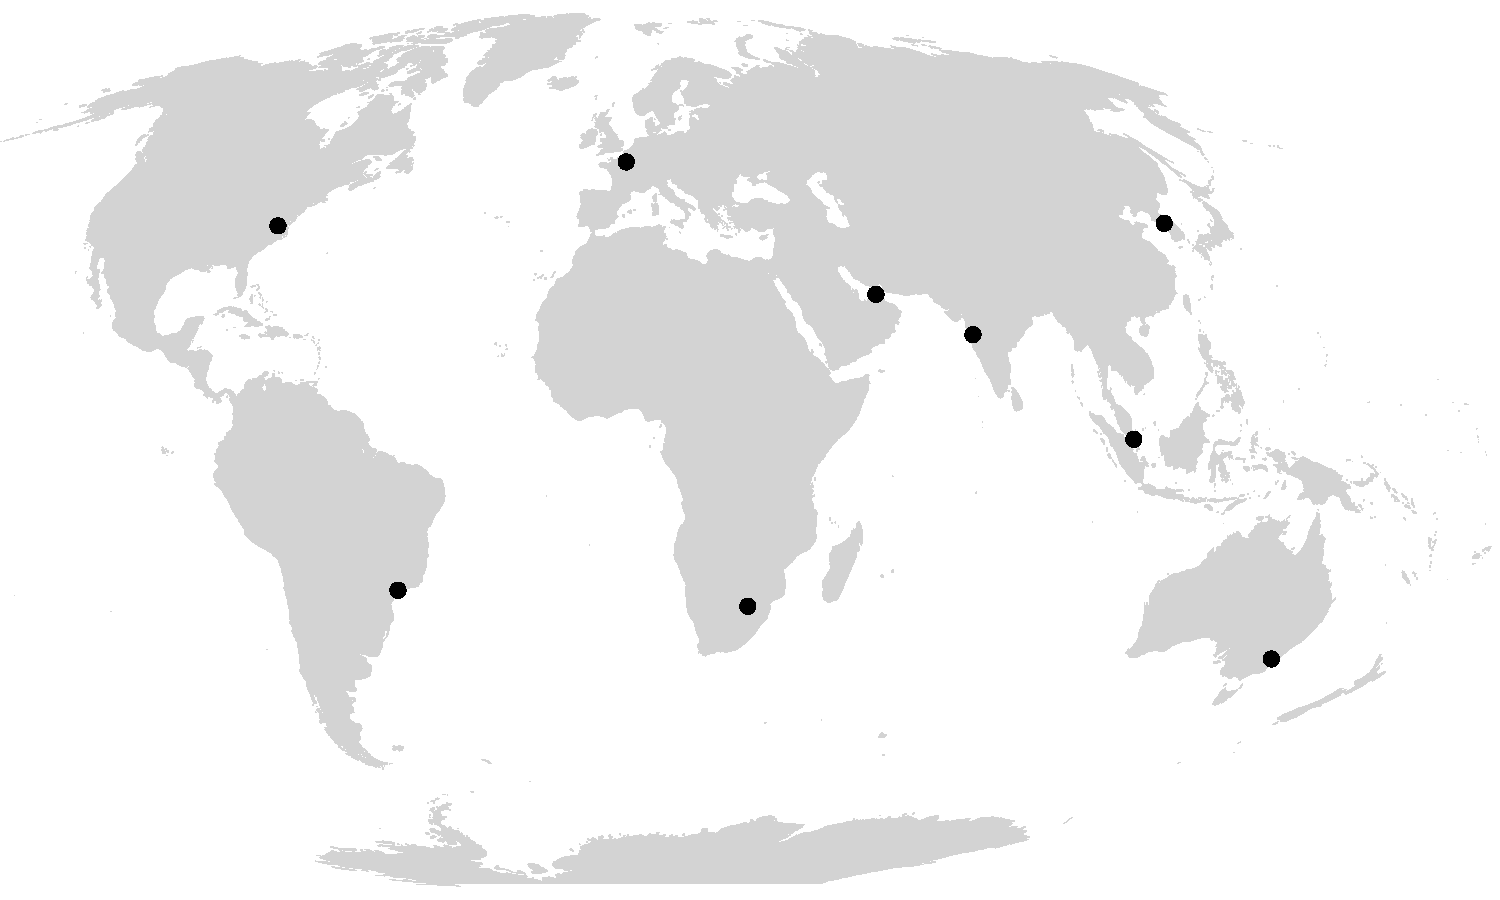
\includegraphics[width=.5\textwidth]{images/locations.pdf}}
\put(40,45){São Paulo}
\put(120,40){Johannesburg}
\put(200,30){Canberra}
\put(200,70){Singapore}
\put(200,105){Seoul}
\put(45,105){Virginia}
\put(110,117){Paris}
\put(130,95){Dubai}
\put(170,85){Pune}
\end{picture}
\caption{Selected locations for the data centers.}
\label{fig:dc_location}
\end{figure}






We used values for the PUE inspired by real data from Microsoft Azure for each region: for the Americas, the PUE is 1.17 (DCs São Paulo and Virginia), Asia Pacific has a PUE of 1.405 (DCs Pune, Canberra, Singapore, and Seoul), and for the Europe region, Middle East, Africa the PUE is 1.185 (DCs Johannesburg, Dubai, and Paris)~\cite{walsh2022_azurepue}. 


% \tdvs{Why do we use P.U.E ant not PUE in the notations? For everything else we don't use points : PV, DC, MW, ... Second question: P.U.E or P.U.E.? Both are used....}


%\begin{table}
  
 % \caption{Selected locations for the data centers.}\label{tab:dcs} \centering

  %\begin{tabular}{|l|r|r|}
    
  %\hline

  %\textbf{Location} &  \textbf{Latitude} & \textbf{Longitude} \\
 % \hline
  %Johannesburg & -26.20500 & 28.04972 \\
 % \hline
 % Pune & 18.52143 & 73.85445 \\
%  \hline
%  Canberra & -35.29759 & 149.10127\\
%  \hline
%  Dubai & 25.26535& 55.29249 \\
 % \hline
 % Singapore & 1.35711 & 103.8195\\
 % \hline     
 % Seoul & 37.56668 &  126.97829 \\
% \hline
%  Virginia  & 37.12322& -78.49277 \\
 % \hline
 % São Paulo &  -23.48620 &  -46.50092  \\
%  \hline 
%  Paris &  48.85889 & 2.32004 \\
 % \hline
    
%\end{tabular}
%\end{table}



\subsubsection{Workload}

The workload used was generated using the Grog generator\footnote{\url{https://pypi.org/project/grog/}},  a workload generator based on analysis of properties of the execution trace made available by Google in 2011~\cite{DACOSTA2018_grog}. For reproducibility purposes, the parameters regarding the number of tasks were set to 350,000, the duration was 30 days, and it was executed 12 times (1 per month). The tasks have a duration of one hour.


\subsubsection{Photovoltaic power production}

Global Solar Horizontal Irradiation (in Wh/m$^{2}$) data was collected from the MERRA-2 project~\cite{GELARO2017MERRA2}, since it provides information for anywhere on earth. Figure~\ref{fig:pv_ghi} illustrates different solar irradiation of each location throughout the year 2021.%\tddc[noinline]{Figure 1 is too small. Make its width as close to linewidth as possible}

 \begin{figure}[!htbp]
  \centering
   {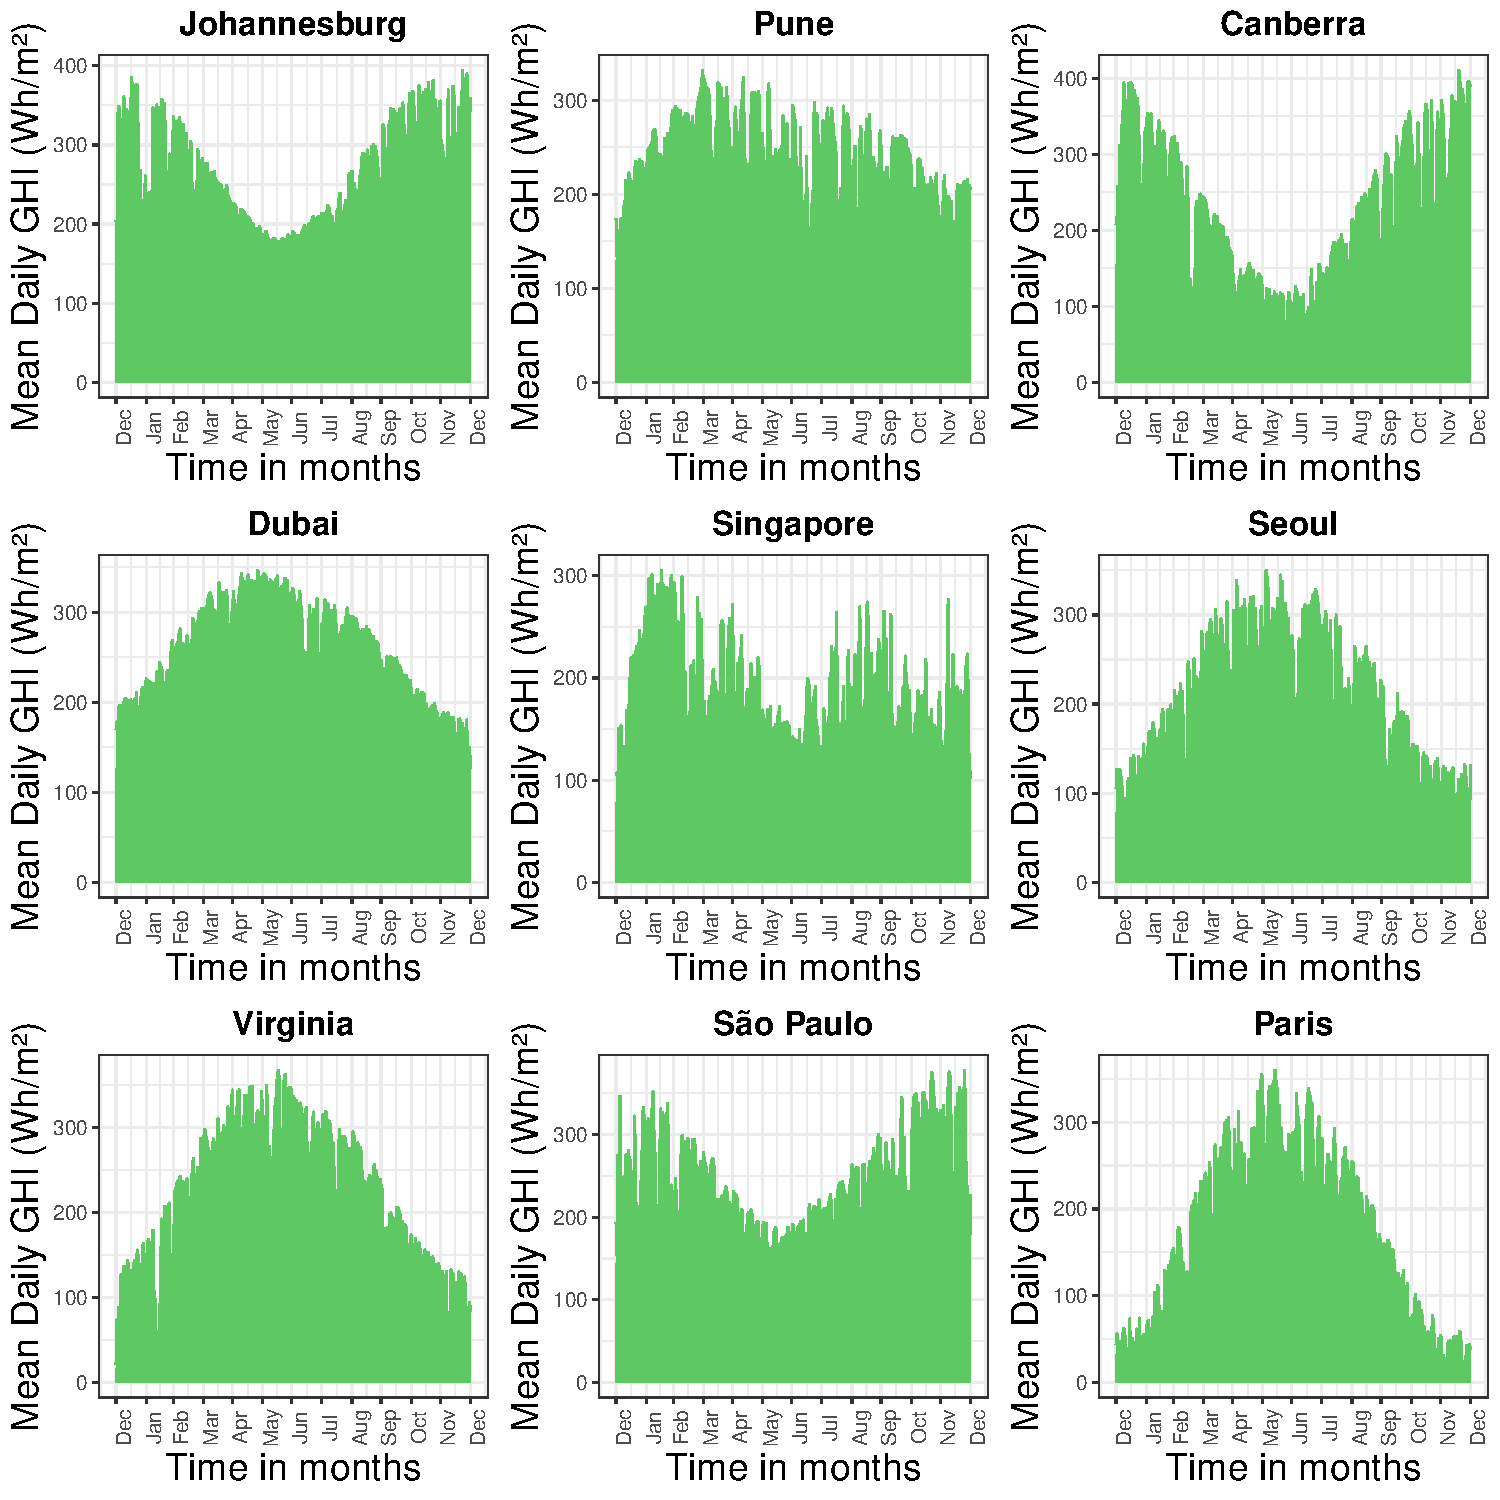
\epsfig{file = images/pv_ghi.pdf, width = \linewidth}}
  \caption{Average daily solar irradiation per location throughout the year 2021.}
  \label{fig:pv_ghi}
\end{figure}

\subsubsection{Carbon footprint}

For solar panels, it is considered a lifetime of 30 years, and manufacturing $1 m^2$ emits $250 kg\,\ch{CO2}-eq$, inspired from real measurements~\cite{YUE2014pv_carbon}. To compute the emissions in the form of $g\,\ch{CO2}-eq.kWh^{-1}$ as stated in Section~\ref{sec:footprintmodel}, we considered the total solar irradiation that was produced during the year 2021 multiplied by 30 (to account for the PV module lifetime of 30 years). For the electrical grid, we also considered the real-world data of the carbon footprint ($g\,\ch{CO2}-eq.kWh^{-1}$). Table~\ref{tab:carbonfootprint} lists the carbon emission values for each region.


\begin{table}
  
  \caption{Emissions (in $g\,\ch{CO2}-eq.kWh^{-1}$) for both PV usage and using the regular grid. Source for grid emissions: electricityMap, climate-transparency.org.}\label{tab:carbonfootprint} \centering

  \begin{tabular}{|l|r|r|}
    
  \hline

  \textbf{Location} &  \textbf{Grid} & \textbf{PV} \\
  \hline
  Johannesburg & 900.6 & 24.90 \\
  \hline
  Pune & 702.8 & 27.96 \\
  \hline
  Canberra & 667.0 & 29.71 \\
  \hline
  Dubai & 530.0  & 24.84 \\
  \hline
  Singapore & 495.0 & 36.19 \\
  \hline     
  Seoul & 415.6 & 34.00 \\
  \hline
  Virginia  & 342.8 & 31.71 \\
  \hline
  São Paulo &  61.7 & 27.99\\
  \hline 
  Paris &  52.6  & 39.93 \\
  \hline  

\end{tabular}  
\end{table}

Regarding the batteries, the emissions are only considered for the manufacturing step---$59 kg\,\ch{CO2}-eq$ per kWh. In our experiments, the considered lifetime of the batteries is ten years. Therefore, the input used is equal to $5.9 kg\,\ch{CO2}-eq$ per kWh, given that we simulated one year.


\subsubsection{Execution environment}
We ran the experiments on a machine with an Intel i9-11950H CPU, and 32 GB of RAM. The solver used was the Gurobi Optimizer (version 9.5.2). The execution time for solving the LP with the inputs listed in the previous sections --- which resulted in a total of 394,263 variables --- was in the order of 30 seconds.
%The experiments were executed on a machine with the following configurations: Intel i9-11950H CPU, and 32 GB of RAM. The solver program used for solving the LP was the Gurobi Optimizer (version 9.5.2). The execution time for solving the LP with the inputs listed in the previous sections---which resulted in a total of 394,263 variables---was in the order of 30 seconds.


\subsection{Results}

In this section, we present the results in terms of the computed optimal area of the PVs and capacity of the batteries, the source of energy that was consumed by the DCs operation (grid, batteries, or PV panels), and the total emissions of the cloud operation, generated from both manufacturing PVs and batteries, and power consumption of the regular electrical grid. Furthermore, to assess the solution computed by the LP, we compare it with two other scenarios: i) only power from the regular electrical grid is used to supply the DCs (represent current DCs), and ii) only power generated from the PV panels, and stored and discharged from the batteries are used to supply the DCs. Finally, we present an evaluation using metrics to assess the environmental impact of the results.


\begin{figure}[!htbp]
  \centering
  {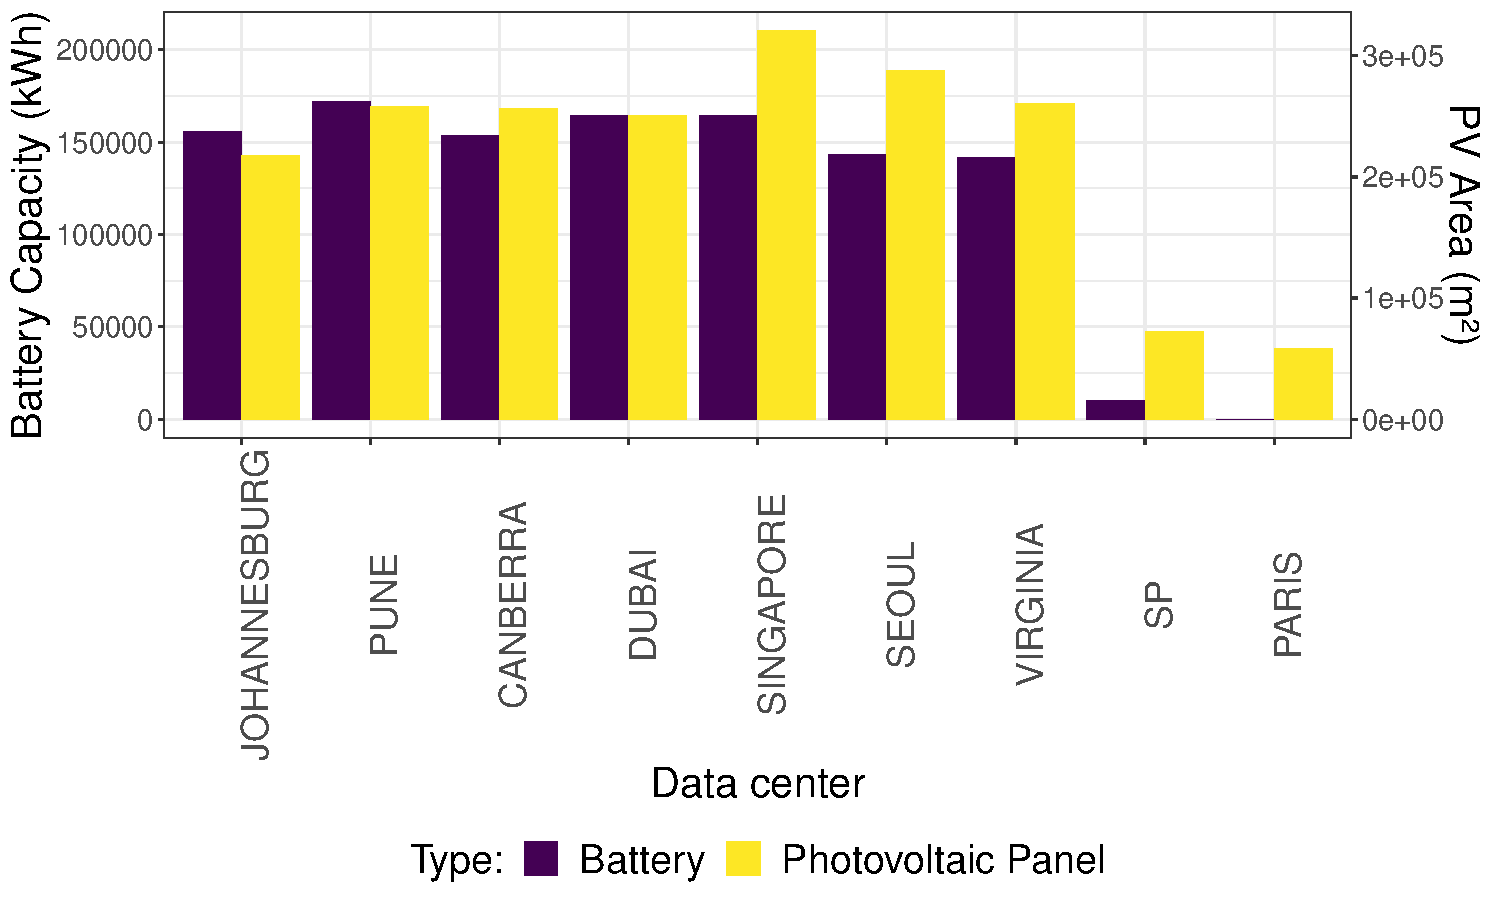
\epsfig{file = images/sizing.pdf, width = .5\textwidth}}
  \caption{Optimal result for the area of PV panels and capacity of the batteries.}
  \label{fig:sizing}
\end{figure}

Figure~\ref{fig:sizing} illustrates the area of the photovoltaic panels and the capacity of the batteries computed from the LP using the inputs described in Section~\ref{sec:experiments}. %These results can be explained by the characteristics of each location in terms of how carbon intensive is the power from the regular electricity grid and how much solar irradiation is received throughout the year: the DCs where the local electricity grid is low-carbon intensive, as São Paulo and Paris, had the smallest area of PVs and capacity of batteries. On the other hand, the DCs with a high-carbon-intensive grid had the highest computed areas and batteries to avoid using the local grid. Singapore had the highest PV area for two reasons: i) the electricity from the regular grid is carbon intensive, and ii) in the year 2021 it was the second worst location in terms of solar irradiation received (Paris was the location that received the less solar irradiation). 

To analyze the sources of energy that supplied the DCs operation, we present in Figure~\ref{fig:energy_ratio_daily} the percentage that each source (grid, renewable, and batteries) was used to daily supply the DCs throughout the year. Figure~\ref{fig:power_ratio_hourly} is a fine-grain visualization of the DC operation regarding the power consumed or produced: it illustrates hour-by-hour the DC total power demand, how much power was consumed from the  grid, discharged from the batteries, and produced by the PV panels.


%Figure~\ref{fig:energy_ratio_daily} illustrates the source of the energy that supplied the DCs operation throughout the simulated year: for each day, it is possible to see the share  %For most data centers, the primary energy source is the power produced from the locally installed photovoltaic panels and stored in the batteries. The usage of grid electricity in the DCs of Virginia, Seoul, and Canberra can be justified by the seasonal intermittency of renewable energy: for Virginia and Seoul --- that is in the northern hemisphere of the globe --- the winter occurs during the first and last months of the year, and for Canberra --- that is in the southern hemisphere of the globe --- the winter occurs during the middle months of the year. The exceptions are the data centers of São Paulo and Paris, where most of the energy consumed was from the regular electrical grid, given that it is low-carbon intensive.


\begin{figure}[t]
  \centering
   {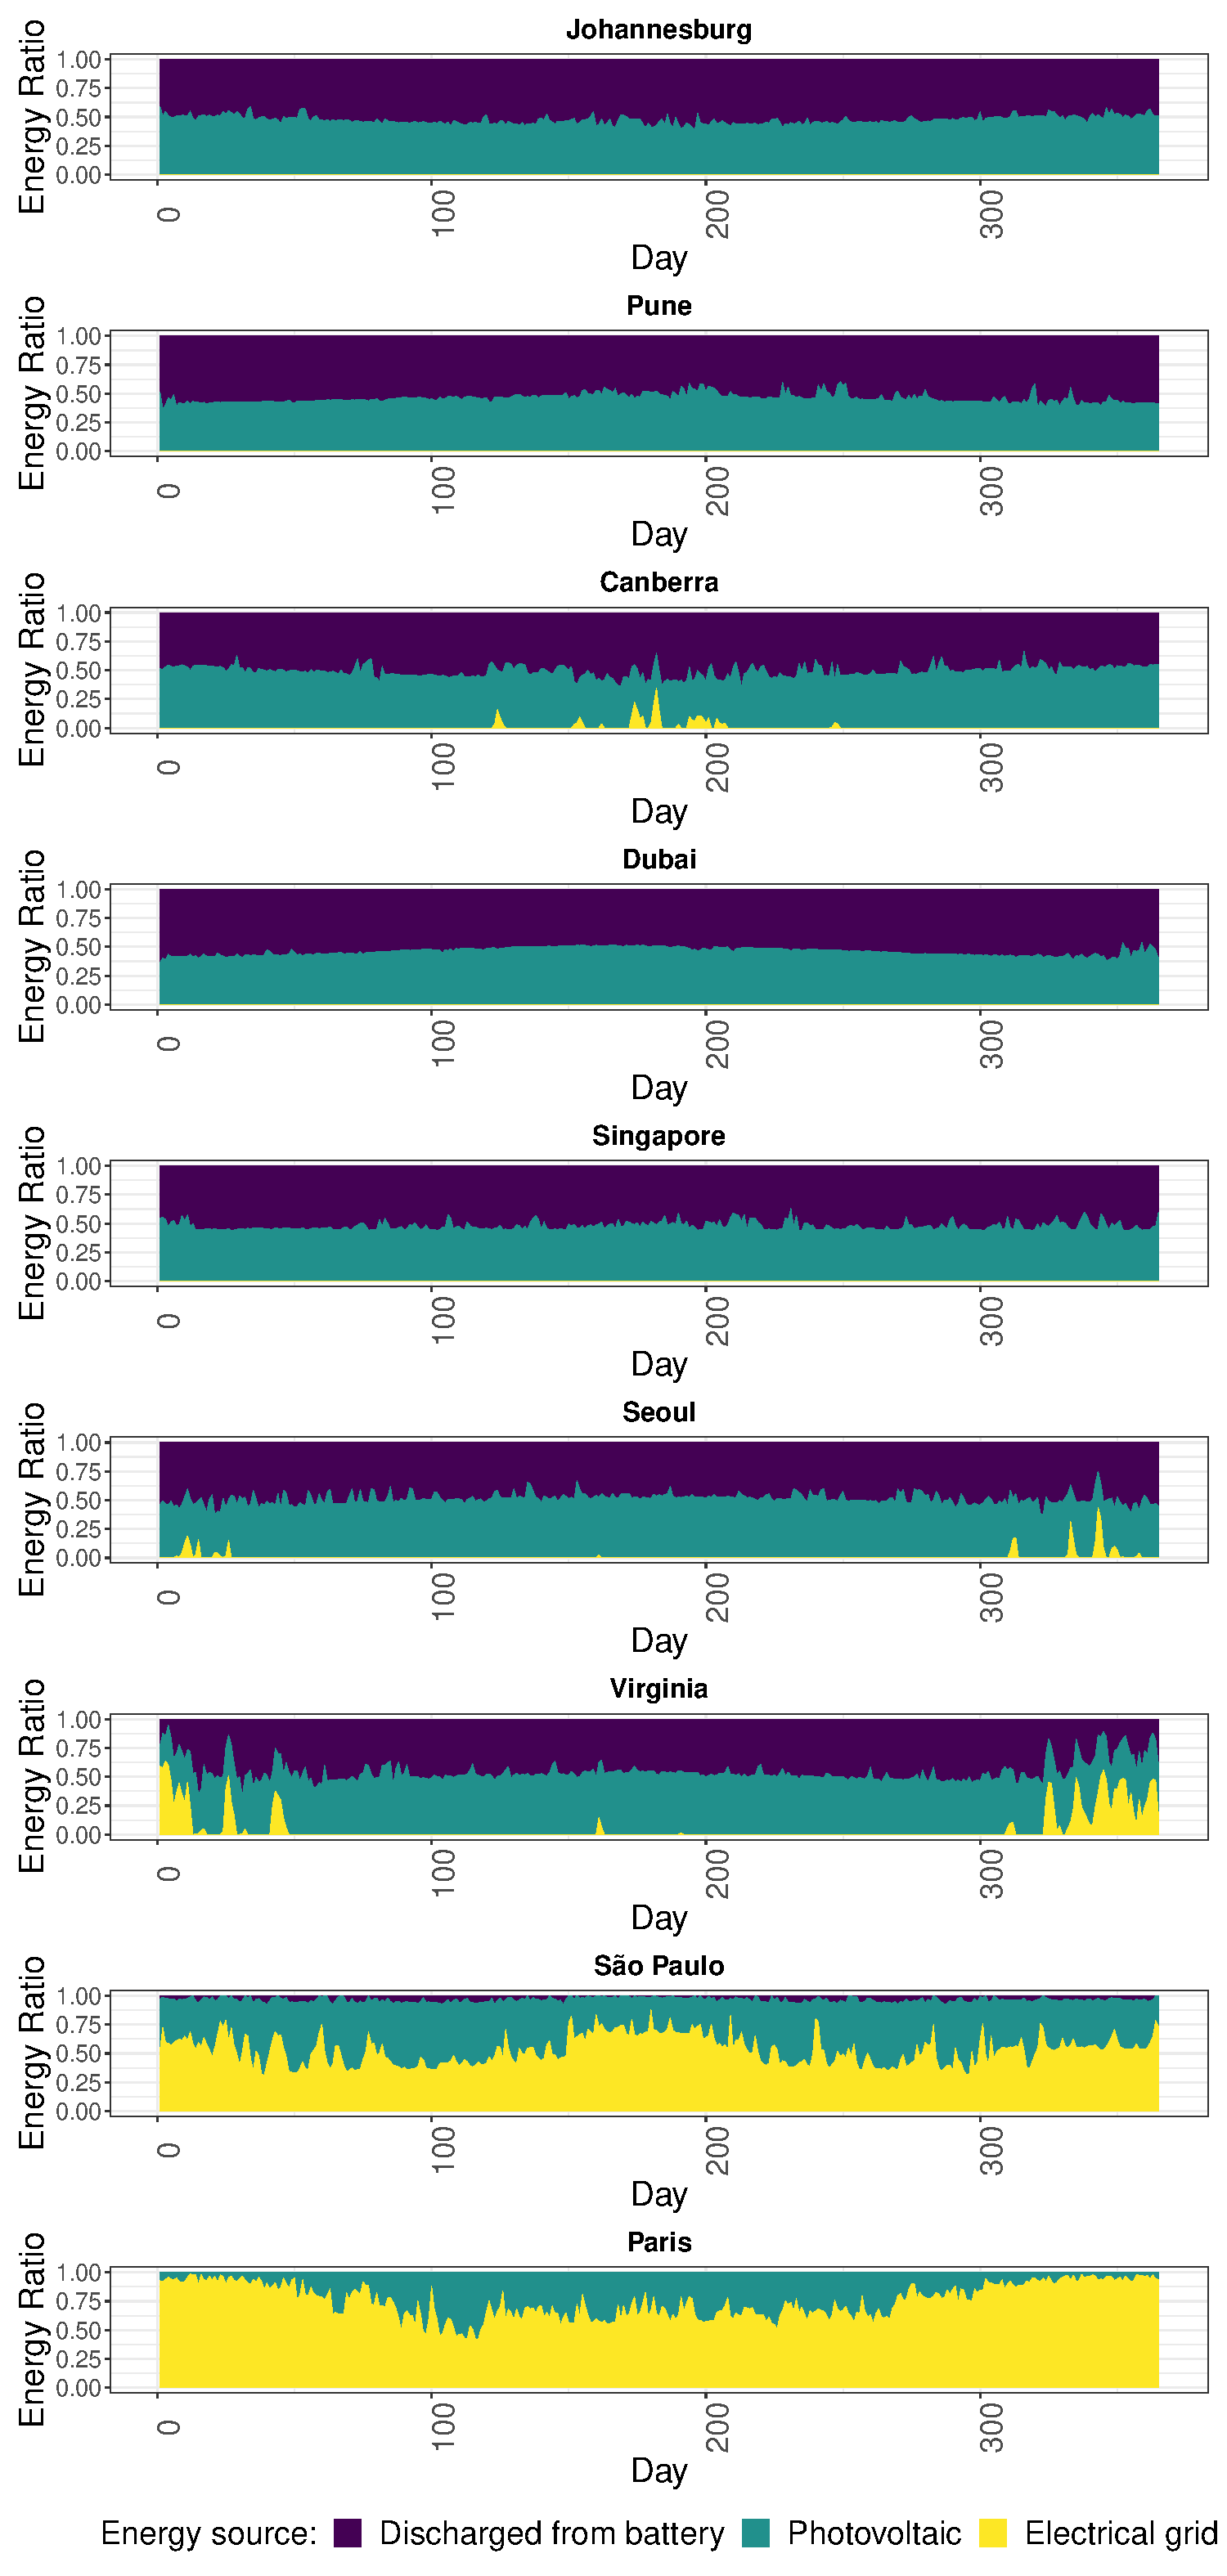
\epsfig{file = images/energy_ratio.pdf, width = .47\textwidth}}
  \caption{Composition of the DCs' daily energy consumption throughout the year considering the different sources of energy, where 1.0 is the DC's total energy consumption.}
  \label{fig:energy_ratio_daily}
\end{figure}


%Figure~\ref{fig:power_ratio_hourly} is a fine-grain visualization of the DC operation regarding the power consumed or produced: it illustrates hour-by-hour the DC total power demand, how much power was consumed from the local electricity grid, discharged from the batteries, and produced by the solar panels. %We can observe how the batteries are used: the power is discharged when there is insufficient renewable power production to supply the DC. It is also possible to observe that the PVs are overproducing power---the PV power production is higher than the DC power demand at some instants of time---to store the electricity in the batteries to use when opportune.



 \begin{figure}[t]
  \centering
   {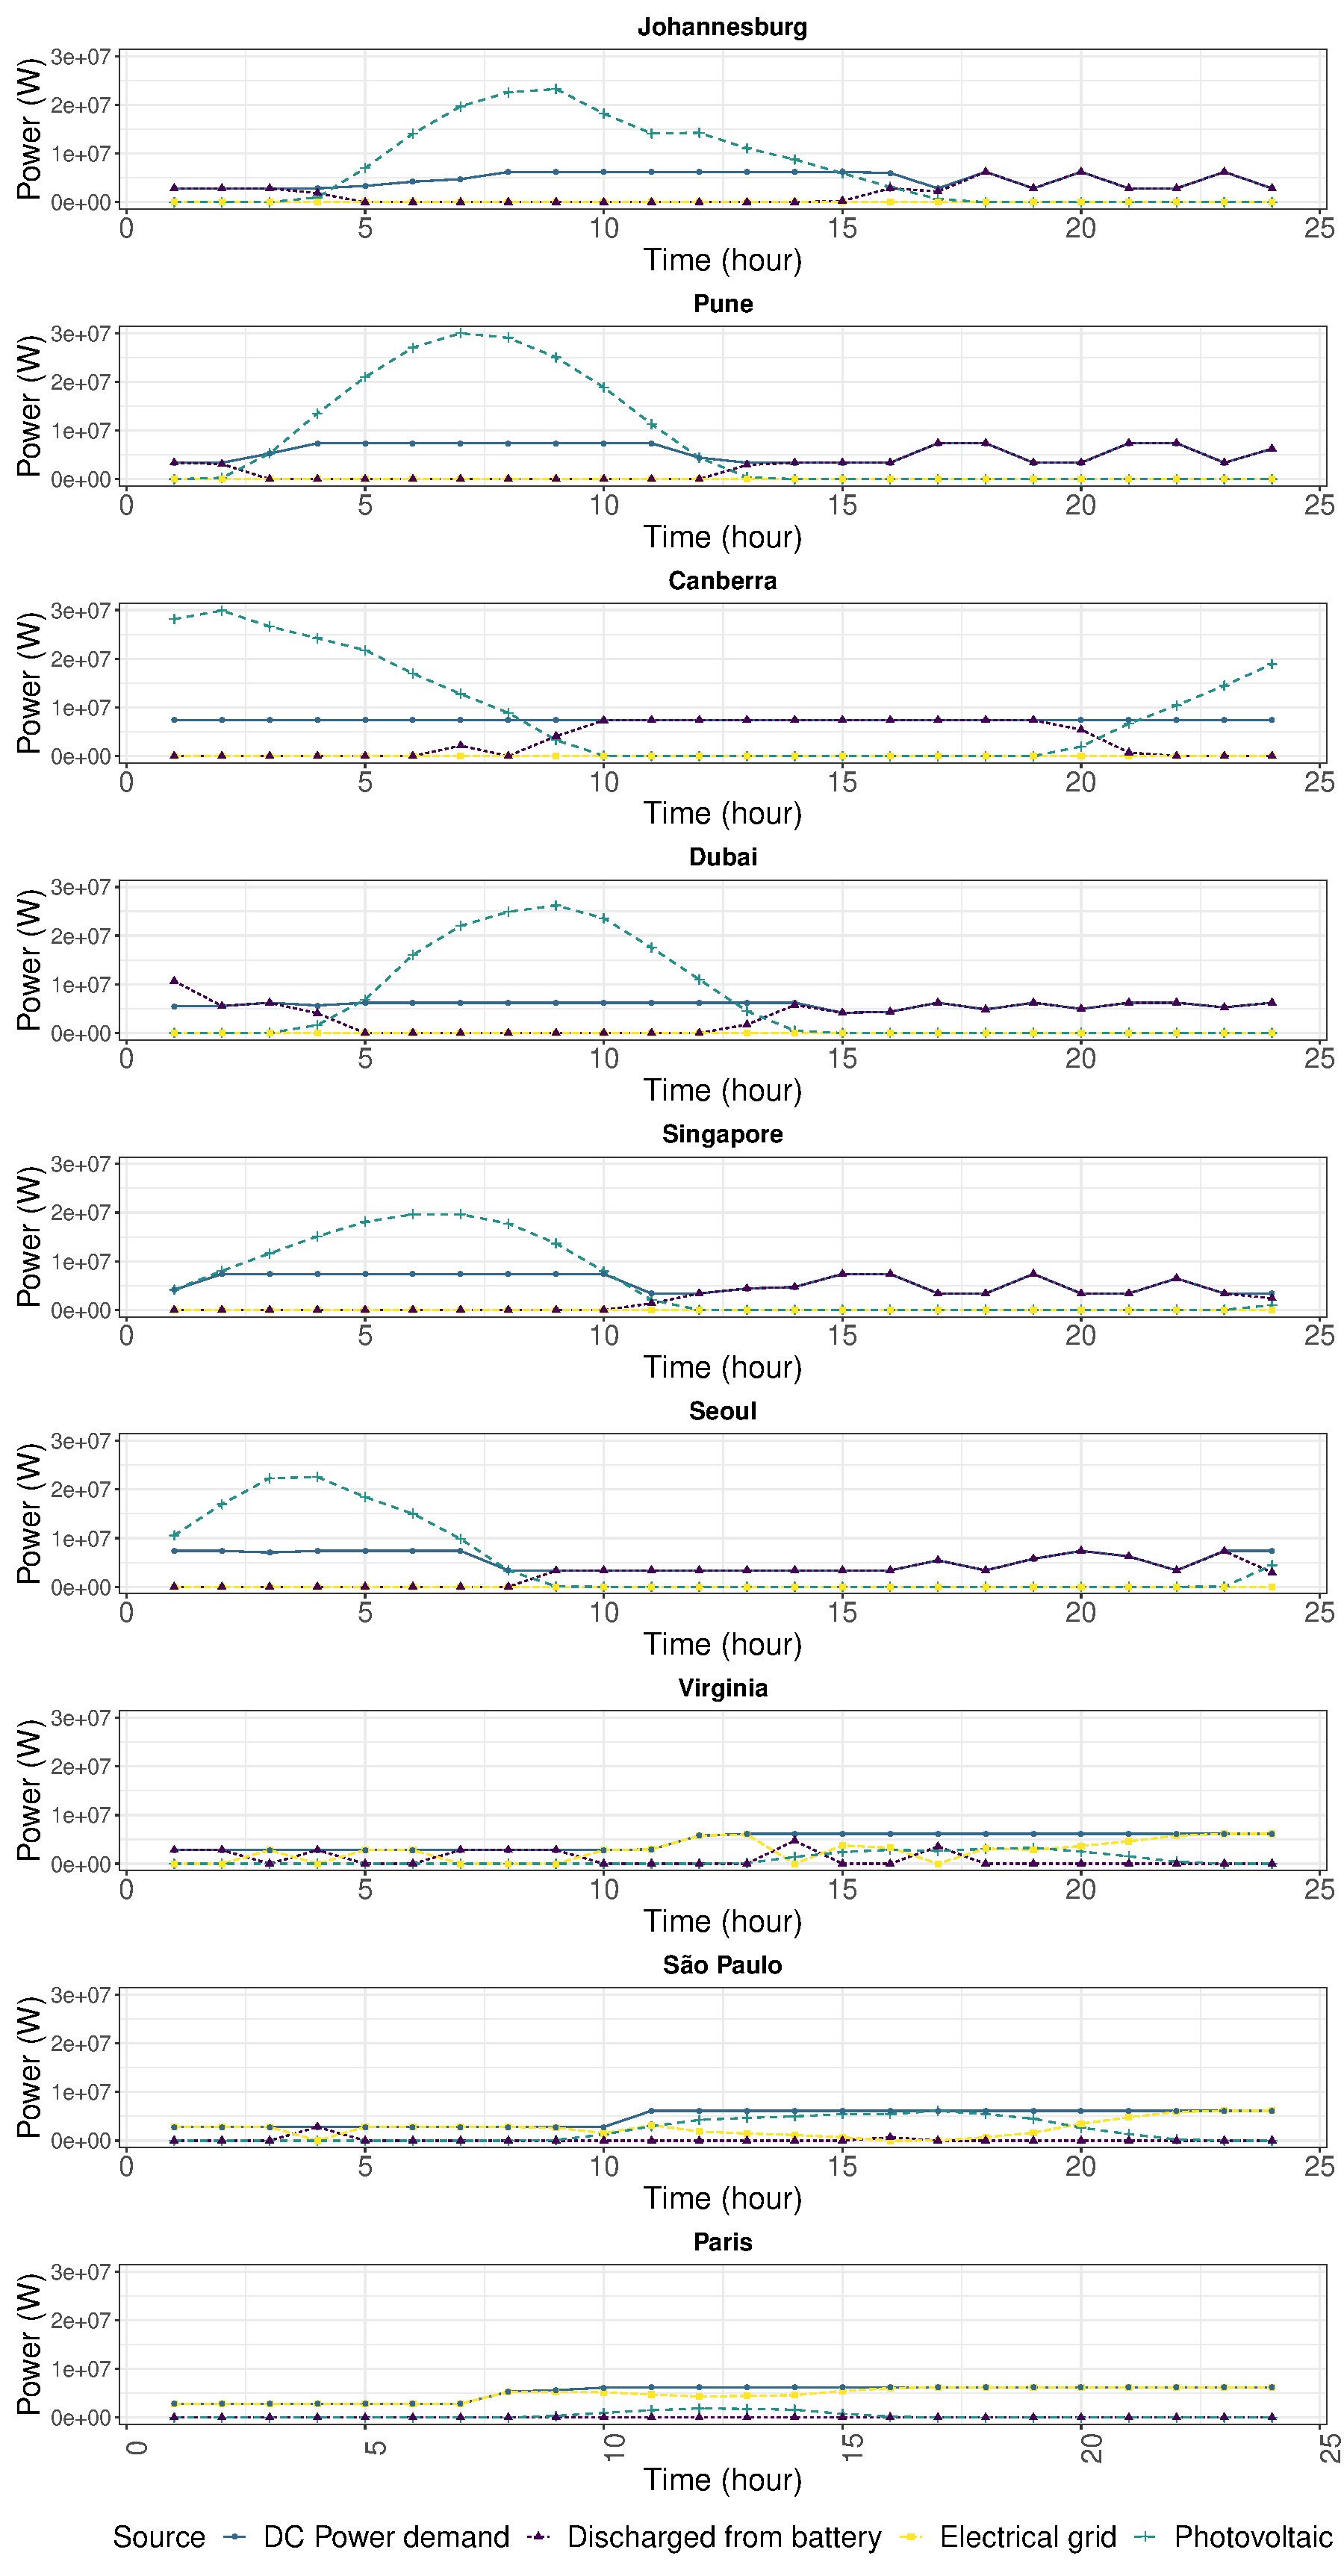
\epsfig{file = images/power_source_hour.pdf, width = .5\textwidth}}
  \caption{Composition of the DCs' hourly power consumption throughout the first day of the year. Time follows the Universal Time (UT) standard.}
  \label{fig:power_ratio_hourly}
\end{figure}

 %The use of the follow-the-renewables approach in a cloud that has data centers distributed across the world can also be observed in Figure~\ref{fig:power_ratio_hourly}: at the instant of time 11 hours (UT), the photovoltaic production in Seoul decreases because the sun is setting. We can also observe that the power consumption of this data center --- which is directly related to the executed workload --- decreases. At the same instant of time, the power consumption in the data center of São Paulo increases, which suggests that the workload was scheduled to be executed there instead of the data center of Seoul, probably to avoid discharging its batteries or using the carbon-intensive local electricity grid at that instant of time. The same behavior can be observed for the data centers Paris and Seoul for the instant of time 8h (UT), and Virginia and Pune for the instant of time 12h (UT).

%\tddc{Shouldn't it be UTC for Coordinated Universal Time instead of UT?}
%\tdmv{The source of data for irradiation is in UT: https://www.soda-pro.com/web-services/meteo-data/merra/info}

In order to assess the optimal solution of the LP, we compared it with two other scenarios in terms of total carbon emissions ($t\,\ch{CO2}-eq$): i) the DCs are only supplied by power from the regular electrical grid, and ii) the DCs are only supplied by power from the photovoltaic panels and batteries. Table~\ref{tab:emissions} presents the results. In comparison with the first scenario (only grid power), the reduction in the \ch{CO2} emissions was approximately 85\%, and it was approximately 30\% for the second scenario (only renewable power).


% Second figure illustrates more detailed

\begin{table}[!ht]
\caption{Total emissions for the different scenarios.}\label{tab:emissions} \centering
\begin{tabular}{|p{5cm}|r|}
  \hline
  \textbf{Scenarios} & \textbf{Emissions ($t\,\ch{CO2}-eq$)}   \\
  \hline
  Electrical grid                    & 201211.3    \\
  \hline
  PV and batteries  &                  42370.6 \\ %40054.1 \\
  \hline
  PV, batteries, and grid            &  29600.6   \\
  \hline


\end{tabular}
\end{table}

%The results shown in Figure~\ref{fig:energy_ratio_daily} can be used to justify these reduction values in comparison to the solution computed by the LP: for the first scenario, the data centers in Paris and São Paulo are already supplied mostly from the energy of the local electricity grid, therefore they didn't have a high reduction in emissions in comparison to the other DCs. On the other hand, for the second scenario, the power from the PVs and batteries already supplies the majority of the DC's power demand, so the additional emissions resulted from manufacturing additional PVs and batteries for the DCs of  Seoul, Virginia, Canberra, São Paulo and Paris --- which is the location that receives the less amount of solar irradiation throughout the year, needing a high area of PV panels to produce power.


To further evaluate these scenarios, we present in Table~\ref{tab:dcutilization} results in terms of the average load each DC executed throughout the year. Equation~\eqref{eq:dcload} represents how the metric was computed for each DC $d$.

\begin{equation}\label{eq:dcload}
\frac{\sum_k w^d_k} {C^d \times K }
\end{equation}


\begin{table}[!ht]
  
  \caption{Average DC load throughout the year }\label{tab:dcutilization} \centering

  \begin{tabular}{|l|r|r|r|}
   \hline
    
  \textbf{Location} &   \textbf{Grid} & \textbf{PV + Bat} & \textbf{PV + Bat + Grid}  \\
  \hline
  Johannesburg & 0 & 79.31  & 86.20  \\
  \hline
  Pune  & 10.25 &  82.07 & 89.34   \\
  \hline
  Canberra  & 99.72 & 66.62 & 67.95 \\
  \hline
  Dubai   & 99.97 & 93.93 & 95.11   \\
  \hline
  Singapore & 99.93 & 72.6  & 85.18 \\
  \hline     
  Seoul    & 99.99 & 81.87 & 65.39      \\
  \hline
  Virginia   & 100.0 & 88.54 & 75.51 \\
  \hline
  São Paulo   & 100.0 & 63.67 & 59.06 \\
  \hline 
  Paris    & 100.0 & 81.24  &  86.11    \\
  \hline  

\end{tabular}  
\end{table}



% \subsubsection{Metrics}

%\tdjmn{Are solutions acceptable ? so which metrics can help the decision marker to accept the plan ? energy waste... everything for the discussion below...}

% possible metrics:
%\tdmv{suggestion of possible metrics:}

To evaluate the environmental impact of the solution, we used metrics extracted from \cite{reddy2017_metrics}. The first metric, the Green Energy Coefficient (or GEC), is the ratio between the total green power generated and the DC total energy consumption, and it can illustrate the oversizing of the green power supply infrastructure. The second metric is the \ch{CO2} savings, which represents the emissions reduction after DC equipment upgrade or flexibility mechanisms. \ch{CO2} savings is computed as seen in Equation~\ref{eq:co2savings}, where: $CO2_{current}$ represents the system studied after the modifications (the result of the linear program for the sizing of PVs and batteries) and $CO2_{baseline}$ the system in its original state. Here, it was considered that $CO2_{baseline}$ has the same workload allocation of  $CO2_{current}$; the difference between the two is that  $CO2_{baseline}$ does not have PVs and batteries, and thus only consumes power from the grid. Table~\ref{tab:metrics} shows the computed values for both metrics. 






\begin{equation} \label{eq:co2savings}
  CO2_{savings} = \left( 1 -  \frac{CO2_{current}} {CO2_{baseline}} \right) \times 100 
\end {equation}



\begin{table}[!ht]
  
  \caption{Results of the sustainability metrics for the experiments}\label{tab:metrics} \centering

  \begin{tabular}{|l|r|r|}
    
  \hline

  \textbf{Location} &  \textbf{GEC} & \textbf{\ch{CO2} savings (\%)} \\
  \hline
  Johannesburg & 1.47 & 93.93 \\
  \hline
  Pune & 1.45 & 91.5 \\
  \hline
  Canberra & 1.57 & 89.59 \\
  \hline
  Dubai & 1.59  & 89.1 \\
  \hline
  Singapore & 1.42 & 85.75 \\
  \hline     
  Seoul & 1.53 & 82.51 \\
  \hline
  Virginia  & 1.46 & 75.99 \\
  \hline
  São Paulo &  0.5 & 20.05 \\
  \hline 
  Paris &  0.24  & 5.25 \\
  \hline  

\end{tabular}  
\end{table}


In order to assess the robustness of the sizing process for the area of PV panels and the capacity of the batteries, it is necessary to take into account other meteorological conditions, given that the DCs will operate for decades and not only for one year. The metric selected is the Mean Absolute Percentage Error (MAPE)  defined by: $ \frac{1}{n}\sum_{i=1}^{n}  \frac{| R_{i} - F_{i}|}{R_{i}}$, where $n$ represents the number of values being considered, $i$ the index of the value being considered, $R_{i}$ the real value for the year, and $F_{i}$ the estimated value (in this case, the computed sizing for the year 2021 that was used in the experiments). Table~\ref{tab:years_MAPE} presents the results of the MAPE for both the area of PV and capacity of the batteries when we solve the LP using as input the solar irradiation for the years 2018, 2019, and 2020. Results indicate a variation of less than 10\% in the different DCs over the years.



\begin{table}[!ht]
  
  \caption{Evaluating sizing for different years using the MAPE metric (values are in \%) }\label{tab:years_MAPE} \centering

  \begin{tabular}{|l|r|r|}
   \hline
    
  \textbf{Location} &   \textbf{PV Area} & \textbf{Battery Capacity} \\
  \hline
  Johannesburg & 1.72 & 1.64  \\
  \hline
  Pune  & 3.72 & 0.76  \\
  \hline
  Canberra  & 8.62 & 4.25 \\
  \hline
  Dubai   & 2.31 & 2.88   \\
  \hline
  Singapore & 7.22 & 0.34 \\
  \hline     
  Seoul    & 3.15 & 1.11 \\
  \hline
  Virginia   & 2.2 & 0.87 \\
  \hline
  São Paulo   & 5.81 & 8.05 \\
  \hline 
  Paris    & 2.76 & 0     \\
  \hline  

\end{tabular}  
\end{table}



%     _                _           _                       _ 
%    / \   _ __   __ _| |_   _ ___(_)___    __ _ _ __   __| |
%   / _ \ | '_ \ / _` | | | | / __| / __|  / _` | '_ \ / _` |
%  / ___ \| | | | (_| | | |_| \__ \ \__ \ | (_| | | | | (_| |
% /_/   \_\_| |_|\__,_|_|\__, |___/_|___/  \__,_|_| |_|\__,_|
%                        |___/                               
%  ____  _                        _             
% |  _ \(_)___  ___ _   _ ___ ___(_) ___  _ __  
% | | | | / __|/ __| | | / __/ __| |/ _ \| '_ \ 
% | |_| | \__ \ (__| |_| \__ \__ \ | (_) | | | |
% |____/|_|___/\___|\__,_|___/___/_|\___/|_| |_|
%
\section{Analysis and Discussion}
\label{sec:analysis-discussion_ccgrid}

These results permit the evaluation of the carbon footprint impact of different electricity supply policies for Clouds. On the one hand, as shown in Table~\ref{tab:emissions}, there is a significant reduction to obtain by including renewable energy in the electricity sources of DCs. We observe a 5-fold decrease in the footprint in our experiments. % This reduction is intuitive
Many Cloud providers have committed to using 100\% renewable energy supplies for their DCs in the following years. On the other hand, this objective of 100\% renewable is, in our opinion, more ideological than pragmatic, and there is more benefit to obtain by combining grid and renewable electricity. We observe in our experiments a further reduction of a fourth in the optimal solution compared to the 100\% renewable scenario. This study thus gives further insight into the debate of energy sources in Clouds.


The locations used in this paper for the different DCs allow us to benefit from the diversity of latitudes, hemispheres, and climates, as shown in Figure~\ref{fig:dc_location}. This variety of longitudes and hemispheres permits mitigation of the impact of seasonal and daily variations of solar irradiation on electricity production and always has at least some DCs with good PV production, as shown in Figure~\ref{fig:pv_ghi}. The diversity of climates is highlighted by the case of Singapore's solar production, which is the second lowest with Paris, while its location close to the equator could permit better irradiation.


% The locations used in this paper for the different DCs allow us to benefit from the diversity of latitudes, hemispheres, and climates. As shown in Figure~\ref{fig:dc_location}, the model includes 3 DCs in the southern hemisphere, 5 in the northern one, and Singapore almost on the equator. Considering the longitudes, two DCs are on the American continent, two on the African and European longitudes, while the 4 last ones are geographically distributed on the Asian and the Australian continents. This variety of longitudes and hemispheres permits mitigation of the impact of seasonal and daily variations of solar irradiation on electricity production and always has at least some DCs with good PV production, as shown in Figure~\ref{fig:pv_ghi}. The diversity of climates is highlighted by the case of Singapore's solar production, which is the second lowest with Paris, while its location close to the equator could permit better irradiation.

As indicated in Table~\ref{tab:carbonfootprint}, we observe significant heterogeneity in the carbon footprint of grid electricity of the different DCs, %Paris and S\~ao Paulo have the lowest electricity footprint, close to 50 g \ch{CO2}-eq/kWh, four DCs with a grid footprint between 300 and 600 g \ch{CO2}-eq/kWh (Virginia, Seoul, Singapore, and Dubai), Pune just over 700 g \ch{CO2}-eq/kWh and the most carbon-intensive grid electricity is in Johannesburg with more than 900 g \ch{CO2}-eq/kWh.
%This heterogeneity 
which results in two categories for the optimal solution: i) Paris and S\~ao Paulo, DCs with a reduced number of PVs and batteries (no battery in Paris), and ii) the other locations have quite similar sizes of PV and batteries. In the second category, the larger PV area is mainly associated with low solar irradiation. It might appear counterintuitive to allocate more PVs to locations with lower solar production, but this is more comprehensive considering the static part of the power consumption of DCs. When the workload is mainly sent to locations with solar production, the electricity consumption of DC also includes a static part for the idle consumption of servers and the interconnection network, as referred to in Equation~\eqref{eq:power_cons}. This static electricity consumption implies either using the carbon-intensive grid or a sizing of PV and batteries that matches the demand, even during winter days of low PV production. This results in a large PV and battery sizing --- the PVs are producing up to 1.6 times the DC energy consumption  as seen in Table~\ref{tab:metrics} --- and, as shown in Figure~\ref{fig:energy_ratio_daily}, the grid energy consumption of these DCs is very low. 


The results for Paris and S\~ao Paulo show the carbon footprint of ESDs compared to grid electricity. There is a small benefit in S\~ao Paulo for intensive usage, so with reduced sizing, there is no benefit in Paris to using batteries. The PV sizing on these DCs is reduced, probably due to the fact that little energy can be stored in case of overproduction.

The detail of hourly electricity consumption is highlighted in Figure~\ref{fig:power_ratio_hourly}. The workload is allocated in DCs with PV production. If all this production is used, or the corresponding DCs are full, then the allocation is driven by the battery state of charge, and when none of these possibilities are available, the allocation is for the DC with the lowest grid electricity footprint. For example, in the last hours, the electricity consumption of the different DCs is furnished by battery discharge, in the limit of a state of charge, and the remaining is allocated in the DCs of Paris, S\~ao Paulo, and Virginia. Thus, the DC of Virginia consumes grid electricity in two cases: either when Paris and S\~ao Paulo DC are full (from hours 10 to 24), or when the DC is empty and only local electricity can be used (hours 3, 5, and 6 in Figure~\ref{fig:power_ratio_hourly}). The follow-the-sun approach can be partially observed between hour 7 and 8, when Seoul PV production fall and the workload is transferred to Paris, with grid consumption.  Then, at hour 10, the same append between PV production in Singapore and grid electricity in S\~ao Paulo and at hour 11 between Pune and Virginia. The figure also shows the impact of location, season, and PV sizing on the solar production between Pune and Canberra, large PV production in the best hours, and the tiny production in Paris.

Table~\ref{tab:dcutilization} presents the impact of the different scenarios for energy sources on the load of the different DCs. In the first scenario, the workload is only allocated based on the grid electricity footprint. Thus, we could expect the workload order to be the same as the footprint order per kWh. However, the consumption does not only depend on the workload but also the PUE of the different DCs. We can thus observe a higher workload in Dubai compared to Singapore, considering that Dubai has electricity with a slightly higher footprint but the lowest PUE. Globally, the range of values highlights the workload variations, requesting at least 4 DCs, at most 8, and most of the time 7. The second scenario considers a model without grid electricity. The allocation is surprisingly distinct from the solar irradiation of the different DCs. For example, the DC of Paris has the lowest yearly irradiation but the median workload in this scenario. Its workload is higher than the one in Johannesburg, which has the second-highest yearly irradiation and is on a similar longitude. The workload is thus not only driven by yearly irradiation. The extremely low PV production in Paris during winter, associated with the static part of the electricity consumption in each data center, implies a high sizing of PV and battery, which lead to a high production during the other seasons that permit a large workload. On Johannesburg, the seasonal variation is lower, so static constraints do not drive PV sizing. Another surprising result is that the DCs with the lowest workload in this scenario are the 4 in the southern hemisphere (including Singapore). This contradicts the intuition of ``follow-the-summer'' allocation. The case of S\~ao Paulo and Canberra could be similar to the one of Johannesburg with the value of the minimal daily production in Virginia and Seoul. The largest workload concerns DCs with the more stable production (Dubai and Pune) and the lowest minimum daily production (Virginia, Paris, and Seoul). Finally, for the last complete scenario, the DCs with the largest workload are the 3 with the largest irradiation (Dubai, Pune, and Johannesburg), followed by Paris with the lowest grid electricity footprint. The only surprise is the workload of S\~ao Paulo, which is low considering its low grid electricity footprint and high solar irradiation, and the workload of Singapore, which is high considering its low PV production. Concerning S\~ao Paulo, this is probably because it has the second-lowest grid footprint. This implies a low battery sizing, thus a low PV sizing, and finally, it mainly receives workload only when no more DC can provide electricity from PV or battery discharge, and when the DC of Paris is full, that makes many constraints. Considering Singapore, it is probably due to its position close to the equator, which implies no ``winter'' season, and its large PV sizing. Finally, the reduction of carbon footprint of each DC between the complete scenario (PV + bat + grid) and the scenario with only grid electricity is showed in Table~\ref{tab:metrics}. It shows a small decrease in Paris and S\~ao Paulo, and a large decrease in the other locations, correlated to the electricity footprint.

%\tdfd{add comments on the results on the different years}
%\tdmv{suggestion of intuitive and non intuitive results}

%Intuitive:

%\begin{itemize}

  %\item Regions with carbon-intensive grid energy needed more PV and batteries, and regions with low carbon-intensive (as Paris and São Paulo) didn't need as much (Figure 2).
  %\item Most data centers are supplied by solar energy to avoid using the grid because it is carbon intensive. With the exception of Paris and São Paulo (with low-carbon intensive electricity), the usage of grid power happened in the winter, when there is less solar irradiation in the location of the DCs (figure 3)
  %\item When the solar power production rate for a time slot drops at a given DC x, the power consumption at dc x also drops, and the power consumption increases at the next time slot at a DC y (follow the renewables approach as seen in Figure 4)
  %\item Using only power from the grid generate significantly more carbon emissions (table 5)
%  \item the locations with the highest carbon-intensive grid had the highest co2 savings
%  \end{itemize}

 
%Non-intuitive:

%\begin{itemize}
%\item the scenarion with grid + pv and batteries resulted in less carbon emissions than the scenarion with full pv and batteries, because the emissions from manufacturing are often neglected (table 5)
%\item in the full grid scenario, Dubai had a higher average load than Singapore, even if it had a lower carbon-intensive grid  (table 6), because of difference of the PUE value, that is, even if the energy is less carbon-intensive, more power will be consumed to cool the DC
%\item São Paulo has the second most lower carbon-intensive regular grid, however was the DC less used (with the smaller average load) (table 6), maybe other regions receive more irradiance, or because they produce more green energy given that they have more pvs and batteries, and therefore use less the grid
%\end{itemize}


% other Items that can be discussed
%\begin{itemize}
  
%\item Fanny comments on intuitive results of table 6.
%\item Considering the specific characteristics of each region (solar irradiation received throughout the year, energy mix of the regular electricity grid, and the carbon emissions) it is possible to find a better solution than the naive approach of considering 100\% PVs and batteries
%\item the global scenario of modern cloud computing allows us to explore the follow-the-renewables approach and use more green energy (low carbon energy), specifically to deal with the question of intermittency between the seasons and throughout the day (day/night)
%\item Solving the two problems at once: scheduling and sizing, allows for a better result because it includes both operations of the IT part (scheduling the workload) and the electrical part (charging or discharging the batteries)
%\item Metrics shows that including PV and batteries are able to reduce the \ch{CO2} emissions significantly, and for some regions that already have green, there is not a great impact so that decision-makers could prioritize some regions
%moved to conclusion \item flexibility to model other scenarios: more DCs, other values for carbon emissions, carbon emissions per time slot, other workloads, etc ...
  
%\end{itemize}


%   ____                 _           _             
%  / ___|___  _ __   ___| |_   _ ___(_) ___  _ __  
% | |   / _ \| '_ \ / __| | | | / __| |/ _ \| '_ \ 
% | |__| (_) | | | | (__| | |_| \__ \ | (_) | | | |
%  \____\___/|_| |_|\___|_|\__,_|___/_|\___/|_| |_|
%
\section{Summary}
\label{sec:conclusion_ccgrid}

In this paper, we tackled the problem of greening a distributed cloud data center (DC) federation to lower its carbon footprint. The IT part of the cloud platform already exists, and the idea is to add the equipment on site to introduce renewable energy into the brown energy from the classical grid into the power supply of the DCs. Since the sun is shining everywhere on earth, we have proposed photovoltaic panels (PVs) to produce renewable energy and batteries as storage devices to mitigate the intrinsic intermittency of this energy during the day. The question is how to size the PV array and associated battery size, given an existing federation of DCs distributed around the earth.
We have provided a formulation of the problem as a linear program. The particularity of our formulation is that we do not need integer variables; a solution is possible using only real variables given our objective and the context of the problem. As a result, the linear program allows to optimally solve large problem sizes, e.g., minimize the carbon footprint of a nine-site federation, each with its own weather conditions, upon a one-year horizon, hour by hour. We have demonstrated that our program is able to calculate the optimal sizing for PVs and batteries in just a few minutes. Numerous experiments have brought forward results that we have analyzed and discussed to explain what these results express. As an example, an interesting result, depending on the DC locations considered, the optimal solution to reduce the carbon footprint is a hybrid configuration between using PVs and the regular electrical grid. Moreover, batteries are not always mandatory in each location. As an example, an interesting result, depending on the DC locations considered, the optimal solution to reduce the carbon footprint is to maintain an energy mix through a hybrid configuration including both PVs and a classical grid where the production is low carbon instead of proposing an all renewable platform. Moreover, batteries are not always mandatory in each location. Furthermore
Finally, our model has the flexibility to be extended to assess other scenarios (more DCs, other locations, values for  carbon emissions, or workloads) and it may help decision-makers build their strategy to reduce the environmental impact of the cloud operation. 

In future work, we plan to propose a sizing process that also includes the IT part. Since this investment has been made for years, another perspective is to introduce uncertainty into this sizing process to obtain a more robust distributed DC platform that can provide satisfying service to clients even if the weather conditions change and the submitted workload evolves. The goal always being to remain as virtuous as possible.


%=========================================================================================





%\section{Introduction and objectives}

%\section{Methodology}

%\section{Experimental Results}

%\section{Conclusions and future directions}
%\section{Summary}
%============================================================================================================

Cloud computing is an essential component of our modern digital society, given that it supports the majority of services and applications we use. On the other hand, one cannot neglect the environmental impact it presents, which originates both from the energy consumption of its operation---higher than the electricity demand of entire countries---and the life cycle of its infrastructure.

In this thesis, we studied strategies to reduce the environmental impact---in terms of carbon footprint---of operating and sizing cloud federations with data centers geographically distributed worldwide. More specifically, we explored two carbon-responsive strategies: ``follow-the-renewables'' and the sizing of the renewable infrastructure and IT equipment.

This chapter begins by providing an overview of the main contributions made in this thesis, as detailed in Section~\ref{sec:conclusion_summary}. Then, we discuss in Section~\ref{sec:conclusion_future_research} potential opportunities for future research directions that build upon the insights derived from the work presented in this thesis. Finally, Section~\ref{sec:conclusion_dissemination} presents the various ways in which our work has been disseminated, including a list of scientific publications that have emerged from the research conducted in this thesis.


\section{Summary of contributions }

\label{sec:conclusion_summary}

The first main contribution of this thesis is the analysis of the impact of the follow-the-renewables strategy on both energy consumption and network---presented in Chapter~\ref{chap:smartgreens}. This approach is an interesting solution to exploit the geographic distribution of cloud data centers all over the world to reduce high-carbon-intensive electricity consumption. However, the decision to migrate the workload needs to consider the resources involved in this operation, particularly the network. 

We conducted computational experiments to investigate the impact of the follow-the-renewables strategies. These experiments used real-world data for workload, climate conditions, models validated by the scientific community for energy consumption and network usage, and different adaptations of the follow-the-renewables. 

The results demonstrated that migration planning without taking into account the network---in particular, the network topology and usage---will result in network congestion and waste of energy. As seen in Section~\ref{sec:wasted_resources_smartgreens}, the energy wasted could be used to power the servers of cloud data centers, and it also contributes to increasing the environmental impact of the cloud operation. We proposed an algorithm for migration planning that can reduce non-renewable energy consumption while not impacting the network, compared to works from the literature that schedule the workload migration without considering the network.

The second main contribution of this thesis is the model to both size the renewable and IT infrastructure and operate cloud federations with the objective of reducing the carbon footprint---presented in Chapter~\ref{chap:ccgrid} and Chapter~\ref{chap:ccgrid-extension}. 

The initial model proposed in Chapter~\ref{chap:ccgrid} focused on the operation for the short term with one year of duration and the possibility of manufacturing on-site solar panels and lithium-ion batteries to generate renewable power and store it to deal with the intermittency of green power. 

The first key aspect of the proposed solution is that it solves both subproblems---sizing and operating---as a single problem, allowing us to evaluate decisions such as increasing the on-site renewable infrastructure dimensions of a data center or scheduling the workload to different geographic locations using the follow-the-renewables approach.

Another key aspect of the model is that it considers the specific characteristics of the geographic locations of the DCs in terms of climate conditions---the capacity to generate renewable power, cooling needs, and the local grid electricity supply---that may already incorporate low-carbon-intensive power sources. Lastly, the proposed solution does not neglect that manufacturing the renewable infrastructure also presents an environmental impact. 

Through experiments using real-world data for workload, climate conditions, server specifications, location of data centers, and grid energy mix,  we demonstrated that the hybrid solution, which combines the on-site renewable infrastructure and can use power from the local grid, is better in terms of carbon footprint than only operating the DCs using power from the local electricity grid or exclusively power from the on-site renewable infrastructure.

We then extended our modeling for the long term in Chapter~\ref{chap:ccgrid-extension}---which is mandatory given that data centers have operational lifetimes spanning over a decade. We started by improving the modeling to consider the carbon footprint of the entire life cycle of the renewable infrastructure---from manufacturing to discarding or recycling---which provides more accurate information on the environmental impact and reduces oversizing. 

Furthermore, we also evaluated including wind power as an on-site renewable source. Our experiments demonstrated that despite further reducing the carbon footprint, it might not be adequate for on-site renewable production given its requirements in terms of land area, the fact that it increases the uncertainty of the sizing process, and the higher monetary costs for wind power production. Therefore, the best candidates for the on-site renewable infrastructure are solar panels to generate power and lithium-ion batteries to store power to supply at night or during periods with low irradiance. 

We also showed that workload scheduling can mitigate a part of the impact of the errors in the sizing process---caused by the uncertainty of the climate conditions. 

In terms of costs, we showed that adopting on-site renewable infrastructure is cheaper than operating the DCs exclusively with power from the local electricity grid. Additionally, the solution with solar panels and batteries is the best in both environmental and monetary aspects for the cloud operators. 

Our model also enables us to assess the potential carbon reduction by adopting servers from new generations that may be more power-efficient, while also considering the carbon footprint of manufacturing the servers. The model is flexible enough to compare one generation of servers to another or determine what would be the optimal solution given many generations of servers. In the optimal solution, the servers are used over their expected lifetime. This fact can be used as inspiration for extending real-life server usage, since they are computationally powerful, discarding them results in environmental impact, and waiting to replace the servers increases the chance of having a server generation that is more power-efficient and computationally powerful.

Finally, the model was thoughtfully designed to exclusively employ linear variables. This enables the model to be solved optimally in polynomial time and evaluate long-term scenarios in a reasonable amount of time. This efficiency reduces the energy consumption and associated carbon footprint of the sizing process itself. Decision-makers could adopt this model to guide their efforts to reduce the environmental impact of cloud computing platforms.
\section{Future Research Directions}

\label{sec:conclusion_future_research}

As discussed in Section~\ref{sec:conclusion_smargreens}, to further assess the impact of the follow-the-renewables strategies, we also need to take into account the network usage by the workload---that reduces the available bandwidth for the migration process. Additionally, the model can be analyzed for container virtualization technology. Since containers are typically smaller than virtual machines, their migration time is faster. This can result in more tasks being migrated or allow migration to data centers located farther away.


We saw in Chapter~\ref{chap:smartgreens} that applying follow-the-renewables has significant potential for reducing the carbon emissions of the cloud operation. We didn't include it in our modeling for sizing and operating the globally distributed cloud data centers, given the high latency between the network links that connect these data centers, which would result in a long migration time. This analysis needs to be made to evaluate the potential of migrating the workload, given that the DCs located farther away might have more availability of low-carbon intensive sources. One possibility is to have a threshold for the migration time, or migrate only tasks with low priority as batch tasks.


Regarding our proposed approach for sizing and operating cloud federations, one crucial point for the long term is the degradation of the renewable and IT infrastructure and the failure of IT equipment. For the decision to manufacture new servers, the model can be extended to a fine grain at the level of the IT equipment (for example, replacing only a disc that failed). The monetary cost analysis can also be applied to the decision to manufacture or replace new servers, provided that data on the hardware price is accessible. Another possibility is to analyze the sizing process considering the usage of other types of hardware for computations, particularly graphical processors (GPUs) that are widely used for artificial intelligence applications.

We explored the sizing decision for existing cloud federations. Our proposed solution could also be extended to evaluate the placement of new data centers with the objective of minimizing the carbon footprint. For example, given a set of options for locations, their respective characteristics in terms of potential for generating renewable power, climate conditions, cooling needs, workload demand, and server specifications and their associated carbon footprint, it would be possible to perform a comparative analysis of the carbon footprint of each location. The results could be used to guide the decision on the location of the new data center.

Finally, there are other types of environmental impacts other than carbon emissions. For example, cloud computing platforms present impacts in terms of water usage for cooling, resource extraction for manufacturing the integrated circuits and the data center infrastructure, and improper disposal of the IT equipment, which could result in toxic substances being released into the environment. In the first moment, it is necessary to model these types of environmental impacts to generate metrics that will permit us to measure them. Similar to how there are metrics to assess the quality of service, it would be interesting to have metrics to evaluate the environmental impact of these services and applications. In the second step, it will be possible to propose solutions to reduce the environmental impact. For example, these metrics could be incorporated into multi-objective workload scheduling algorithms or included in the sizing process to minimize them.

\section{Work Dissemination}

\label{sec:conclusion_dissemination}

The following two main publications emerged from the work performed during this thesis---both in the format of full papers:

\begin{itemize}

\item  \textit{\textbf{Miguel Felipe Silva Vasconcelos}, Daniel Cordeiro, Georges Da Costa, Fanny Dufossé, Jean-Marc Nicod, and Veronika Rehn-Sonigo. ``Optimal sizing of a globally distributed low carbon cloud federation''. In 2023 IEEE/ACM 23rd International Symposium on Cluster, Cloud and Internet Computing (CCGrid), Bangalore, India, 2023, pp. 203-215. DOI: 10.1109/CCGrid57682.2023.00028}.
  
\item  \textit{\textbf{Miguel Felipe Silva Vasconcelos}, Daniel Cordeiro and Fanny. ``Indirect network impact on the energy consumption in multi-clouds for follow-the-renewables approaches''. In Proceedings of the 11th International Conference on Smart Cities and Green ICT Systems — SMARTGREENS 2022, pages 44–55. INSTICC, SciTePress. DOI: 10.5220/0011047000003203}. Candidate for the best paper award.

\end{itemize}

The work was also disseminated in the form of short summaries and presentations with partial results to receive initial feedback at the following events:

\begin{itemize}

\item \textit{\textbf{Miguel Felipe Silva Vasconcelos}, Daniel Cordeiro, Georges Da Costa, Fanny Dufossé, Jean-Marc Nicod, and Veronika Rehn-Sonigo. ``Long-term evaluation for sizing low-carbon cloud data centers''. In ComPAS 2023 Conférence francophone en informatique, Jul 2023, Annecy, France}

\item  \textit{\textbf{Miguel Felipe Silva Vasconcelos}. ``Towards low-carbon globally distributed clouds''. In GreenDays 2023, ENS Lyon}.

\item  \textit{\textbf{Miguel Felipe Silva Vasconcelos}, Daniel Cordeiro and Fanny Dufossé. ``Dimensioning of multi-clouds with follow-the-renewable approaches for environmental impact minimization''. In 23ème congrès annuel de la Société Française de Recherche Opérationnelle et d’Aide à la Décision (ROADEF 2022), INSA Lyon}.

\item  \textit{\textbf{Miguel Felipe Silva Vasconcelos}. ``Towards greener multi-clouds: scheduling with follow-the-renewables and dimensioning of solar panels and batteries''. In 5th Workshop of the InterSCity Project (INCT of the Future Internet for Smart Cities), São Paulo, 2022.}

\end{itemize}

Finally, the work presented in Chapter~\ref{chap:ccgrid-extension} will be submitted to a scientific journal---the publication was in the writing phase at the time this thesis was written.


%============================================================================================================

%==============================================


\cleardoublepage

% --- BACK MATTER ----------------------

\pagenumbering{arabic}  % arabic page numbering (e.g., 1 2 3), reset counter
\renewcommand*{\thepage}{A\arabic{page}}  % prepend A to appendix page number
%\pagestyle{scrheadings}  % display header and footer
\addtocontents{toc}{\bigskip}  % visual hint for numbering change in ToC

\appendix%
\cleardoublepage

{
	\setstretch{1.1}
	\renewcommand{\bibfont}{\normalfont\small}
        \renewcommand{\bibname}{References}
        \renewcommand{\refname}{References}
	\setlength{\biblabelsep}{0pt}
	\setlength{\bibitemsep}{0.5\baselineskip plus 0.5\baselineskip}
	\printbibliography
}
%\cleardoublepage
\clearpage

% appendix chapters go here
\cleardoublepage
\appendix

\chapter{Résumé étendu en français}


\section{Introduction}

Cloud computing (ou l'informatique en nuage) a révolutionné le monde industriel et académique de la technologie de l'information avec sa capacité à fournir de grandes quantités de ressources informatiques à la demande. La plupart des applications et des services que nous utilisons quotidiennement, qui comptent de plus en plus d'utilisateurs, tels que les réseaux sociaux, le courrier électronique, les jeux vidéo, la banque en ligne, les applications de santé et la diffusion vidéo, sont pris en charge par des plates-formes de cloud computing.


Malgré tous ses avantages, les centres de données en nuage (DC), les installations qui hébergent toute l'infrastructure nécessaire au cloud, ont une demande énergétique significative. L'Agence internationale de l'énergie (AIE) estime que les centres de données qui hébergent les plateformes de cloud computing ont consommé entre 240 et 320 TWh, soit environ 1\% de l'électricité finale mondiale générée en 2022~\cite{IEA_2022}. Pour mettre cette consommation d'énergie en perspective, cela suffit à fournir la demande énergétique annuelle de pays entiers. En 2022, sept pays avaient une consommation énergétique similaire à la demande énergétique des DC : la Grèce (316 TWh), Israël (304 TWh), la Biélorussie (297 TWh), la Suisse (292 TWh), la Hongrie (266 TWh), le Portugal (258 TWh) et le Maroc (257 TWh)~\cite{owidenergy}.

Les efforts à la fois de la communauté académique et de l'industrie tentent de réduire cette gigantesque consommation d'énergie. Une analyse de l'utilisation mondiale de l'énergie par les centres de données réalisée par \citet{masanet2020recalibrating} a montré que pendant la période entre 2010 et 2018, le trafic Internet des DC a augmenté de plus de 10 fois, on estime que la capacité de stockage des DC a augmenté de 25 fois, et la charge de travail et le nombre d'instances de calcul des DC ont augmenté de 6 fois. D'autre part, la consommation d'énergie n'a augmenté que de 6\% grâce aux améliorations suivantes : i) la virtualisation, qui a permis une augmentation de 5 fois du nombre moyen d'instances de calcul par serveur physique ; ii) des serveurs plus économes en énergie (une diminution d'un facteur de 4 en ce qui concerne la puissance utilisée pour le calcul et un facteur de 9 en termes de watts par téraoctet) ; et iii) des infrastructures économes en énergie, en particulier pour les besoins de refroidissement et d'alimentation électrique.



Il est incertain si les améliorations de l'efficacité dans le cloud computing permettront de compenser l'augmentation de la consommation électrique causée par la demande croissante en ressources informatiques à long terme. Dans le travail de \citet{koot2021usage}, les auteurs ont développé un modèle de prévision de la consommation d'énergie des centres de données en utilisant l'approche des modèles dynamiques de système. En considérant la période de 2016 à 2030, et le scénario avec la fin de la loi de Moore, qui prédit que le nombre de composants dans les circuits intégrés double chaque année~\cite{Mack_2011_moorelaw}, et la montée des applications industrielles de l'Internet des objets, la demande énergétique des centres de données pourrait atteindre 2,3\% de la génération mondiale d'électricité, elle doublera par rapport à ce qui a été rapporté par l'AIE pour l'année 2022~\cite{IEA_2022}.


La consommation d'électricité des centres de données a un impact environnemental en termes d'émissions de gaz à effet de serre (GES). Selon l'Agence internationale de l'énergie, 1\% des émissions de GES liées à l'énergie proviennent des centres de données et des réseaux de transmission de données~\cite{IEA_2022}. L'ampleur de cet impact dépend du type de source utilisé pour produire l'électricité. Le tableau~\ref{tab:co2_power_sources} présente les émissions pour les différents types de sources d'énergie pour produire 1 kWh d'énergie. Les émissions sont mesurées en utilisant le métrique de l'équivalent en dioxyde de carbone (ou \ch{CO2}-eq). Cette métrique est utilisée pour comparer différents GES en termes de leur potentiel de réchauffement global (PRG) en utilisant le dioxyde de carbone comme base : le méthane (\ch{CH4}) a un PRG de 25, ce qui signifie que l'émission de 1 g de \ch{CH4} dans l'atmosphère a le même impact environnemental que l'émission de 25 g de \ch{CO2}\cite{eurostat_co2_eq}. On peut observer que la production d'électricité à partir du charbon émet 77 fois plus de \ch{CO2} que l'éolien ou le nucléaire. En 2019, environ 70\% du trafic de données d'Internet était traité par les centres de données dans l'« Allée des centres de données », une région située en Virginie (États-Unis d'Amérique), qui était alimentée par moins de 2\% d'énergie renouvelable (énergie verte)\cite{clicking_clean_virginia}.


Afin de réduire leur impact environnemental, les principaux fournisseurs de cloud, tels qu'Amazon AWS, Apple, Google, Meta (anciennement Facebook) et Microsoft, se sont engagés à intégrer dans leurs opérations des centres de données une électricité à faible intensité carbonée produite par des sources renouvelables, et certains ont déjà déployé leurs projets pour atteindre l'objectif de minimiser l'empreinte carbone. En effet, Google a rapporté qu'en 2022, 64\% de l'électricité utilisée pour alimenter ses centres de données sur une base horaire provenait de sources renouvelables~\cite{google_sustainability_report_2023}, certains centres de données atteignant même jusqu'à 97\% d'utilisation d'énergie verte.
\begin{table}[!ht]

\caption{ Émissions (en g\,\ch{CO2}-eq) de différentes sources d'énergie par kWh d'électricité produite~\cite{nrel_lifecycle_2021}.}\label{tab:co2_power_sources} \centering

\begin{tabular}{|l|r|}
  \hline
  \textbf{Technologie de génération} & \textbf{Émissions ($\mathbf{g\,\ch{CO2}\text{-}eq/kWh}$)}   \\
  \hline  
  Charbon   & 1 010\\  
  \hline
  Pétrole   & 840\\
  \hline
  Gaz naturel   & 486\\
   \hline
  Biomasse   & 52 \\
  \hline
  Photovoltaïque   & 43 \\
  \hline
  Hydraulique & 21 \\
  \hline
  Nucléaire   & 13 \\
  \hline
  Éolien   & 13 \\
  \hline
\end{tabular}
\end{table}


Les plateformes cloud intègrent l'énergie renouvelable dans leurs opérations de différentes manières. Une possibilité est d'acheter de l'énergie verte auprès du réseau électrique local, bien que cela les rende dépendantes du mix énergétique du réseau, et toutes les régions du monde ne sont pas alimentées par des sources à faible émission de carbone. Une autre possibilité est de fabriquer leur propre infrastructure renouvelable sur site. Un aspect critique de la production d'électricité à partir d'énergies renouvelables qui doit être pris en compte pour ces deux possibilités est leur caractère intermittent : leur production fluctue dans le temps et est influencée par des variables telles que l'heure de la journée, le climat, la saison et la localisation géographique. Par exemple, les panneaux photovoltaïques ne produisent de l'énergie que lorsque le soleil brille, et pendant l'hiver, l'irradiation solaire est plus faible que durant l'été. Pour l'hydroélectricité, de longues périodes sans pluie affecteront la production d'énergie.



L'adoption de dispositifs de stockage d'énergie (DSE) dans les centres de données pour stocker l'énergie renouvelable~\cite{wang2012_EDCS} est une approche pour faire face à l'intermittence. Ces dispositifs sont déjà utilisés dans les centres de données comme sauvegarde temporaire en cas de pannes de courant. L'énergie verte provenant des DSE pourrait être utilisée lorsqu'il n'y a pas de production d'énergie verte ou lorsque la demande est supérieure à la production. Néanmoins, cette approche présente également certains défis pour décider quand utiliser ou recharger, étant donné les caractéristiques des DSE, telles que le taux d'autodécharge (ils perdent de l'énergie stockée avec le temps lorsqu'ils ne sont pas utilisés), le vieillissement (leur capacité maximale diminue avec le temps) et les taux de charge et de décharge limités (la puissance maximale pouvant être extraite ou rechargée).



Dans cette thèse, nous étudions comment réduire l'impact environnemental des centres de données de cloud computing, notamment en termes d'émissions de \ch{CO2}. L'utilisation de stratégies sensibles au carbone - des approches conscientes de leur empreinte carbone et utilisant ces informations pour prendre des décisions~\cite{schooler2021carbonaware} - est explorée pour réduire les émissions de \ch{CO2} à la fois dans l'exploitation et dans le dimensionnement des centres de données - en déterminant l'infrastructure renouvelable nécessaire sur site (surface des panneaux solaires, nombre d'éoliennes, capacité des DSE). En ce qui concerne les opérations des centres de données, nous exploitons la planification de la charge de travail en utilisant des approches follow-the-renewables - des stratégies qui migrent et allouent la charge de travail aux emplacements avec une disponibilité d'énergie renouvelable plus élevée~\cite{shuja2016sustainable} - et étudions leur impact à la fois sur la consommation d'énergie et la congestion du réseau. En ce qui concerne le dimensionnement, nous modélisons notre problème en utilisant une formulation de programme linéaire (PL) qui prend en compte les caractéristiques de chaque emplacement de centre de données en termes de besoins de refroidissement et de mix énergétique local du réseau, ainsi que le fait que l'infrastructure renouvelable génère un impact environnemental. Plus de détails sur la structure et les contributions de cette thèse sont présentés dans la section suivante.


Cette thèse est structurée en six chapitres, comprenant ce chapitre introductif. Une vue d'ensemble du contenu de chaque chapitre et de leurs contributions respectives est décrite ci-après.

Dans le Chapitre~\ref{chap:background}, le lecteur est introduit aux concepts nécessaires pour comprendre la recherche réalisée dans cette thèse. En particulier, le chapitre contient une description du scénario général du cloud computing, comment on peut mesurer l'impact environnemental des plateformes cloud, un aperçu des algorithmes d'ordonnancement dans le contexte du cloud computing, et la définition des stratégies sensibles au carbone - particulièrement, les approches explorées dans cette thèse : follow-the-renewables et le dimensionnement. Enfin, les travaux connexes utilisés comme inspiration ou comme bases pour nos solutions proposées sont également présentés dans ce chapitre.

Une analyse de l'adoption de la stratégie sensible au carbone follow-the-renewables et son impact sur la consommation d'énergie et la congestion du réseau est présentée dans le Chapitre~\ref{chap:smartgreens}. La solution proposée consiste en un algorithme qui prend en compte la topologie et l'utilisation du réseau pour planifier la migration de la charge de travail. À travers des expériences computationnelles avec des données du monde réel pour la charge de travail, l'infrastructure cloud, et un simulateur qui utilise des modèles réalistes validés par la communauté scientifique pour la consommation d'énergie et l'utilisation du réseau, les résultats montrent que la solution proposée surpasse les références en termes de consommation d'énergie, de consommation d'énergie non renouvelable et de congestion du réseau.


Le Chapitre~\ref{chap:ccgrid} introduit une stratégie sensible au carbone qui peut être combinée avec le suivi des renouvelables pour réduire l'empreinte carbone des plateformes de cloud computing en exploitation : le dimensionnement de l'infrastructure renouvelable. Cette stratégie consiste à déterminer la surface requise des panneaux solaires sur site et la capacité des batteries pour fournir la demande d'énergie des centres de données.


La solution proposée consiste en une formulation de Programme Linéaire qui aborde à la fois la planification de la charge de travail en utilisant le suivi des renouvelables et le dimensionnement de l'infrastructure renouvelable sur site. En modélisant ces deux sous-problèmes comme un seul problème, il est possible d'évaluer s'il est plus efficace d'exécuter la charge de travail dans d'autres emplacements géographiques ou d'augmenter la surface des panneaux solaires et la capacité des batteries pour atteindre l'objectif de réduction des émissions de \ch{CO2}. Le modèle n'utilise que des variables linéaires, ce qui lui permet d'être résolu de manière optimale en temps polynomial, ce qui est essentiel à l'échelle des plateformes de cloud computing qui comptent des millions de serveurs et exécutent des centaines de millions de tâches computationnelles chaque jour. D'autres aspects importants de la modélisation sont qu'elle prend en compte les caractéristiques de chaque emplacement géographique des centres de données en termes de besoins de refroidissement, le mix énergétique du réseau électrique local (qui peut avoir une part de sources d'énergie renouvelable), et le fait que la fabrication de panneaux solaires et de batteries a un impact environnemental.

Les résultats démontrent que la configuration hybride qui combine à la fois l'infrastructure renouvelable sur site et le réseau électrique régulier surpasse en termes d'émissions de \ch{CO2} les stratégies ayant un centre de données uniquement alimenté par l'énergie produite par son infrastructure renouvelable locale, avec une réduction d'environ 30\%, et n'utilisant que l'énergie du réseau électrique régulier, avec une réduction d'environ 85\%.

Le modèle introduit au Chapitre~\ref{chap:ccgrid} se concentre sur l'exploitation à court terme (une année). Dans le Chapitre~\ref{chap:ccgrid-extension}, nous étendons le modèle pour évaluer comment minimiser les émissions de carbone des opérations des centres de données cloud à long terme.

Les modifications et analyses suivantes ont été réalisées : l'impact environnemental de tout le cycle de vie de l'infrastructure renouvelable (de la fabrication, de l'exploitation et du recyclage) est pris en compte pour rendre le modèle plus proche du monde réel ; une analyse des avantages et des défis liés à l'inclusion de turbines éoliennes dans l'infrastructure renouvelable sur site ; une évaluation de la sensibilité du modèle aux entrées, en particulier les conditions climatiques et les données sur les émissions du réseau ; une analyse de la réduction possible des émissions de \ch{CO2} en adoptant la flexibilité de retarder une partie de la charge de travail, ce qui pourrait être utilisé pour atténuer les impacts du surdimensionnement de l'infrastructure renouvelable ; une discussion des coûts monétaires (en dollars) associés à l'infrastructure renouvelable sur site, ainsi que des compromis entre la minimisation de l'empreinte carbone et la réduction des coûts pour les centres de données ; et décider de fabriquer de nouveaux serveurs au fil des ans qui peuvent être plus économes en énergie, en considérant que leur fabrication émet également du carbone. Cette modélisation peut être utilisée pour guider les décideurs dans leurs efforts pour réduire l'empreinte carbone des centres de données cloud.

Enfin, le Chapitre~\ref{chap-conclusion} présente une discussion des principales contributions de cette thèse, ainsi que des trajectoires de recherche futures possibles.

Dans ce qui suit, nous présentons un résumé des principales contributions de chaque chapitre. Le lecteur peut consulter le manuscrit original (en anglais) pour avoir accès à plus de détails.

%% Background %%%%%%%%%%%%%%%%

\section{Contexte}

Cette section fournit les connaissances fondamentales nécessaires au lecteur pour comprendre les chapitres suivants de cette thèse. Tout d'abord, le scénario général de l'informatique en nuage est présenté dans la Section~\ref{sec:cloud_resume}. La Section~\ref{sec:measuring_environmental_impact_resume} présente comment on peut mesurer l'impact environnemental des plateformes de cloud computing. Ensuite, une introduction à l'ordonnancement dans le contexte des clouds est présentée dans la Section~\ref{sec:scheduling_cloud_resume}. Les approches existantes explorées dans cette thèse pour réduire l'impact environnemental des plateformes de cloud computing sont discutées dans la Section~\ref{sec:carbon_responsive_resume}, et les travaux utilisés dans cette thèse comme inspiration et références sont également présentés. Enfin, la Section~\ref{sec:summary_background_resume} résume cette section.
\subsection{Cloud computing}

\label{sec:cloud_resume}

Le cloud computing a été introduit par l'industrie pour résoudre les problèmes les plus importants du commerce électronique de l'époque. Avant l'avènement du cloud computing et de son accès à la demande aux ressources informatiques, les utilisateurs et les entreprises devaient acheter leur propre infrastructure informatique pour déployer leurs services ou applications. En cas de pic soudain de demandes, il était souvent difficile de mettre à l'échelle l'infrastructure informatique à temps pour gérer la demande de charge informatique. Malgré ses aspects révolutionnaires en technologie de l'information, le cloud computing n'est pas classé comme un nouveau paradigme dans la recherche en informatique. En fait, c'est l'évolution de la recherche dans différents domaines de l'informatique, tels que les clusters, les grilles, l'informatique autonome et l'informatique ubiquitaire.

L'un des éléments critiques qui permettent le cloud computing est la technologie de virtualisation, dans laquelle les ressources informatiques d'une machine physique sont converties en ressources virtuelles pouvant être partagées entre de nombreux utilisateurs et applications, également connue sous le nom de multi-tier. Les principales idées de la virtualisation proviennent de la fin des années 1950 et du début des années 1960 avec le paradigme de multiprogrammation, et aujourd'hui, la recherche sur les machines virtuelles (VM) et les containers continuent d'étudier les compromis décrits dans la littérature de la multiprogrammation en termes de portabilité, de performance et de sécurité~\cite{randall2020_virtualization}.

Les plateformes de cloud computing prennent généralement en charge des services à trois niveaux distincts : IaaS (Infrastructure en tant que Service), PaaS (Plateforme en tant que Service) et SaaS (Logiciel en tant que Service)~\citep{fos08}. Au premier niveau, Infrastructure en tant que Service (IaaS), la plateforme accorde aux utilisateurs l'accès aux ressources matérielles (telles que le traitement et le stockage) et leur facture leur utilisation. Des services tels qu'Amazon EC2 (Elastic Cloud Computing) Service et Amazon S3 (Simple Storage Service) sont des exemples de clouds IaaS. Au deuxième niveau, Plateforme en tant que Service (PaaS), le fournisseur prend en charge un environnement complet de développement, de test et de déploiement pour le développeur d'applications, ce qui signifie habituellement que le développeur devra suivre un modèle de développement spécifique et accepter des restrictions sur la manière de modéliser le logiciel en échange de la scalabilité fournie. Un exemple est le Google App Engine. Enfin, au troisième niveau, Logiciel en tant que Service (SaaS), des applications spécifiques sont proposées aux utilisateurs via Internet, et le tarif est proportionnel à l'utilisation de l'application. Nous pouvons citer les applications de bureautique Google Docs comme exemples.


Les plates-formes de cloud computing modernes sont composées de plusieurs centres de données répartis géographiquement dans le monde entier, également appelés fédérations de cloud ou multi-clouds. La figure~\ref{fig:dc_locations} illustre les emplacements des centres de données cloud de Microsoft Azure qui, au total, sont composés de millions de serveurs physiques~\cite{roach2021_microsoftazure}. Le besoin d'une infrastructure géographiquement distribuée provient de la nécessité de répondre à la demande du grand nombre d'utilisateurs et de réduire le temps de réponse pour leurs applications, ainsi que pour des raisons de sécurité et de redondance. Par exemple, si un centre de données dans une région tombe en panne en raison d'un problème d'alimentation ou d'une attaque de piratage, une autre région pourrait temporairement recevoir la charge de calcul. Enfin, cette infrastructure distribuée permet d'explorer différentes approches pour réduire l'impact environnemental de l'exploitation des centres de données, et plus de détails sur ces stratégies sont donnés dans la section~\ref{sec:carbon_responsive_resume}.


\subsection{Mesurer l'impact environnemental des platesformes de cloud computing}

\label{sec:measuring_environmental_impact_resume}


Le protocole GHG~\cite{ghgprotocol2004} a été développé comme moyen de standardiser la mesure et la déclaration de l'impact environnemental des entreprises. Il prend en compte six types de gaz à effet de serre (GES) du protocole de Kyoto : le dioxyde de carbone (\ch{CO2}), le méthane (\ch{CH4}), l'hexafluorure de soufre (\ch{SF6}), le protoxyde d'azote (\ch{N2O}), les hydrofluorocarbures (HFC) et les perfluorocarbures (PFC).


Le protocole comporte trois domaines pour quantifier les émissions directes et indirectes :

\begin{itemize}
\item \textbf{Scope 1 - Émissions directes de GES} : prend en compte les émissions générées par les sources que l'entreprise possède ou contrôle. Dans le contexte du cloud computing, cela pourrait provenir de l'électricité générée lors d'une surtension, et des générateurs devraient être utilisés comme solution de secours ; le transport des produits, des matériaux et des employés à l'aide des véhicules de l'entreprise ; et le refroidissement de l'infrastructure du centre de données~\cite{gupta2021_chasingcarbon}.
\item \textbf{Scope 2 - Émissions indirectes de GES liées à l'électricité} : prend en compte les émissions générées par l'électricité consommée.
\item \textbf{Scope 3 - Autres émissions indirectes de GES} : Ce domaine est facultatif et prend en compte les émissions issues de la production ou de l'extraction des matériaux et des combustibles achetés, par exemple, les équipements informatiques (tels que les serveurs et les routeurs) ainsi que la construction des installations du centre de données. Les émissions liées au transport sont également incluses dans ce domaine si elles proviennent de véhicules non possédés par l'entreprise.
\end{itemize}  

Les principaux acteurs du cloud fournissent déjà des rapports de durabilité et utilisent le Protocole GHG. Dans le rapport de durabilité de Meta pour 2023~\cite{meta_sustainability_report_2023}, il est estimé que 1\% des émissions proviennent du Scope 1, moins de 1\% du Scope 2 et 99\% du Scope 3. De plus, il est indiqué que les émissions opérationnelles ont été réduites de 94\% par rapport à 2017 grâce aux engagements en matière d'énergie renouvelable. Un autre exemple remarquable est le rapport environnemental de Google pour 2023~\cite{google_sustainability_report_2023}, où il est estimé que 1\% des émissions proviennent du Scope 1, 24\% du Scope 2 et 74\% du Scope 3. Google indique également que la majeure partie des émissions du Scope 3 proviennent de la fabrication du matériel et des biens d'équipement qu'ils ont achetés et de la construction des installations de centres de données.

Dans cette thèse, l'impact environnemental est uniquement évalué en termes d'empreinte carbone, en utilisant la métrique équivalente en \ch{CO2} (\ch{CO2}-eq). Cette décision a été prise en raison du manque de données pour mesurer d'autres impacts environnementaux, tels que l'utilisation de l'eau, et les impacts causés par l'extraction de minéraux bruts pour fabriquer les circuits intégrés.



\subsection{Ordonnancement pour les plateformes de cloud computing}
\label{sec:scheduling_cloud_resume}

Les problèmes d'ordonnancement sont des problèmes d'optimisation combinatoire où, étant donné la description des caractéristiques d'un ensemble de ressources informatiques ($\alpha$) et d'un ensemble de tâches ($\beta$), l'objectif est de trouver une allocation (dans le temps) des ressources aux tâches qui minimise certains critères d'optimisation ($\gamma$). Ces problèmes sont généralement désignés en utilisant la notation \mbox{$\alpha$ $\vert$ $\beta$ $\vert$ $\gamma$}, introduite par Graham~\citep{graham}.

Le critère le plus couramment étudié dans les problèmes de calcul haute performance est appelé makespan (également noté par $C_{\max}$), qui indique le moment où la dernière tâche composant une application termine son exécution. Lorsque les ressources informatiques disponibles sont identiques et connues à l'avance, et que nous cherchons à minimiser le makespan, typiquement le cas dans les problèmes d'ordonnancement dans les grappes et les grilles de calcul, le problème est fortement NP-difficile~\citep{Garey}. Ce problème est désigné par $P,\vert,\vert,C_{\max}$ dans la notation de Graham.

Pour le problème de recherche exploré dans cette thèse, $\alpha$ représente les ressources informatiques (mémoire et CPU) des serveurs des centres de données ainsi que leurs informations sur la disponibilité de sources d'alimentation à faible intensité carbonique, $\beta$ représente les exigences des machines virtuelles en termes de temps d'exécution, de délai, de mémoire et de CPU, et $\gamma$ représente la réduction de la consommation d'énergie carbonée.


Il est connu, d'après les travaux de~\citet{graham} et~\citet{Garey}, que la classe d'algorithmes gloutons connus sous le nom d'algorithmes de liste fournit des heuristiques rapides et efficaces pour l'ordonnancement des tâches sur des ordinateurs parallèles. Ces algorithmes ont une garantie d'approximation de $2 -1 /m$ dans le pire des cas, mais sont remarquablement efficaces en pratique, surtout lorsque le rapport entre le nombre de tâches et le nombre de ressources informatiques disponibles est élevé. Parmi les algorithmes de liste les plus couramment utilisés, on trouve le Longest Processing Time first (LPT) et le Shortest Processing Time first (SPT), pour les plateformes homogènes, et l'algorithme Heterogeneous Earliest Finish Time (HEFT), pour les plateformes hétérogènes.

La stratégie de consolidation des machines virtuelles illustre un exemple de problème d'ordonnancement dans le cloud computing rendu possible par la virtualisation. Elle consiste à utiliser des migrations en direct, migrer la VM entre différentes machines tout en étant en cours d'exécution, c'est-à-dire sans préemption, pour réallouer les VM afin d'atteindre le nombre minimum de machines physiques utilisées, et éteindre les machines devenues inactives pour économiser de l'énergie. Le lecteur peut consulter le travail de~\citet{10.1145/3470972} pour une revue systématique de la littérature sur de telles techniques.

Les algorithmes gloutons ont été adoptés dans certaines des solutions proposées dans cette thèse, ainsi que dans la plupart des travaux connexes utilisés comme bases et sources d'inspiration. La justification de cette décision est que, bien qu'ils ne fournissent pas la solution optimale, ils peuvent fournir une solution acceptable dans un laps de temps raisonnable, ce qui est important compte tenu de la taille de la charge de travail avec des millions de tâches et des restrictions telles que la date limite, le temps de réponse, et autres. La section suivante présente ces stratégies au lecteur.



\subsection{Carbon-Responsive Computing}

\label{sec:carbon_responsive_resume}

De nombreux efforts, tant de la part du milieu universitaire que de l'industrie, sont déployés pour réduire l'impact environnemental des technologies de l'information. Le terme \guillemotleft Carbon-Responsive Computing\guillemotright a été créé pour décrire les stratégies qui explorent le déplacement de la charge de travail informatique à la fois dans le temps et dans l'espace dans le but de réduire l'empreinte carbone de l'opération~\cite{schooler2021carbonaware}.

Il existe trois niveaux de Carbon-Responsive computing. Dans le premier, Carbon-aware computing, le système connaît l'intensité carbone de l'électricité utilisée par ses charges de travail ou son équipement informatique. Dans le second, carbon-responsive computing, les informations sur l'intensité carbone sont prises en compte pour prendre des décisions. La dernière étape, carbon-resilient computing, étudie comment gérer et intégrer des éléments réactifs au carbone et quelles modifications sont nécessaires dans l'informatique et l'infrastructure d'alimentation pour réduire l'empreinte carbone.


Dans cette thèse, une étude de la stratégie carbon-aware follow-the-renewables est présentée (Section~\ref{sec:followtherenewables_resume}), ainsi que la stratégie carbon-resilient de dimensionner l'infrastructure renouvelable (Section~\ref{sec:sizing_resume}).


\subsubsection{Follow-the-renewables}

\label{sec:followtherenewables_resume}

Comme nous l'avons vu dans la Section~\ref{sec:cloud_resume}, les plates-formes de cloud computing modernes sont réparties géographiquement à travers le monde, ayant des centres de données dans de nombreuses combinaisons de latitudes, de longitudes et de fuseaux horaires. Étant donné que chaque emplacement a un potentiel différent pour générer de l'énergie renouvelable, et que l'énergie renouvelable est intermittente - le soleil ne brille que pendant la journée, et le vent ne souffle pas tout le temps à des vitesses suffisantes pour faire tourner les pales des éoliennes - les algorithmes de planification peuvent utiliser cette caractéristique pour planifier l'exécution de la charge de travail dans les endroits où il y a plus de disponibilité d'énergie verte. Dans la littérature, le terme \guillemotleft follow-the-renewables\guillemotright~\cite{shuja2016sustainable} describes this strategy. Cette stratégie se concentre sur le Scope 2 du Protocole GHG, car elle planifie la charge de travail à l'emplacement qui utilise moins d'énergie intensive en carbone provenant de sources renouvelables.


%\guillemotleft and \guillemotright
\subsubsection{Dimensionner l'infrastructure renouvelable}


\label{sec:sizing_resume}


Il existe deux options principales pour répondre à la demande d'électricité à faible intensité en carbone de la fédération cloud. Le propriétaire du centre de données peut acheter de l'électricité verte auprès du réseau électrique local intégrant les énergies renouvelables, ce qui les rend dépendants du réseau, et toutes les localisations ne permettent pas cette possibilité, ou il peut installer une infrastructure renouvelable locale dans les centres de données. Pour cette dernière option, le principal problème est de décider des dimensions de l'infrastructure renouvelable nécessaire, par exemple, la surface requise des panneaux solaires, le nombre d'éoliennes et la capacité des batteries (pour stocker l'énergie verte et l'utiliser lorsque c'est opportun) pour alimenter le centre de données et minimiser son empreinte carbone. Ce problème est connu sous le nom de dimensionnement ou de planification de la capacité dans la littérature (sizing, dimensioning ou capacity planning en anglais). De nombreux facteurs doivent être pris en compte dans la décision de dimensionnement : les coûts de fabrication et d'exploitation de ces appareils, le potentiel de production d'énergie compte tenu des conditions climatiques et de la localisation géographique, et le fait que ces appareils présentent également un impact environnemental tout au long de leur cycle de vie ne peut être négligé.

La stratégie de dimensionnement de l'infrastructure renouvelable prend en compte les Scopes 1, 2 et 3 du Protocole GHG : les émissions de carbone directes de la production d'électricité dans le centre de données, les émissions liées à la consommation d'électricité du réseau électrique ordinaire, et les autres émissions de GES indirectes provenant de la fabrication et du cycle de vie de l'infrastructure renouvelable et de l'équipement informatique.

%%%% SMARTGREENS
\section{Follow-the-renewables et leur impact sur le réseau et la consommation énergétique}


L'approche \guillemotleft follow-the-renewables\guillemotright (le lecteur peut consulter le Chapitre~\ref{chap:background} pour plus de détails) est une stratégie intéressante pour atténuer l'intermittence de la disponibilité de l'énergie renouvelable sans avoir besoin d'utiliser des dispositifs de stockage d'énergie. Par exemple, lorsque c'est la nuit dans l'emplacement où se trouve un centre de données A, la charge de travail pourrait être migrée vers un autre centre de données B où le soleil brille encore pour utiliser l'énergie solaire, comme illustré dans la Figure~\ref{fig:ex_follow_the_renewables}.

Malgré ses avantages, on ne peut négliger les limitations de la stratégie follow-the-renewables. Tout d'abord, le processus de migration d'une machine virtuelle entre différents centres de données consomme lui-même de l'énergie : il utilise des dispositifs réseau (comme des commutateurs et des routeurs) et une tâche informatique pour le processus de migration en direct. L'algorithme de planification doit prendre en compte cette consommation d'énergie avant de décider si la migration est avantageuse. Deuxièmement, les liens de communication réseau qui connectent les serveurs à l'intérieur du centre de données et les différents centres de données peuvent souffrir de congestion, ce qui peut augmenter la durée de la migration. Cela entraîne une computation et une consommation d'énergie inutiles à la fois sur les serveurs d'origine et de destination : le serveur qui envoie la machine virtuelle doit attendre la fin du processus de migration pour libérer ses ressources et recevoir des machines virtuelles supplémentaires, ou il pourrait également être éteint pour économiser de l'énergie ; le serveur qui reçoit la machine virtuelle ne commencera à exécuter la nouvelle machine virtuelle qu'après la fin du processus de migration. Un algorithme de planification efficace doit prendre en compte ces facteurs pour réduire l'empreinte carbone des opérations des centres de données.

Le travail de Camus et al.~\citet{SAGITTA,NEMESIS} a étudié la planification de la charge de travail en nuage, sous forme de machines virtuelles (virtual machine ou VM en anglais), sur des centres de données géographiquement répartis afin de minimiser la consommation d'énergie non renouvelable. Il a proposé différents modèles stochastiques pour estimer la production d'énergie renouvelable et des algorithmes heuristiques gloutons pour allouer des tâches aux serveurs. Les VM peuvent être migrées pendant leur exécution vers un ordinateur situé dans le même centre de données (consolidation des serveurs intra-DC) ou vers un ordinateur dans un centre de données situé dans un autre emplacement géographique (\guillemotleft follow-the-renewables\guillemotright). L'algorithme de planification prend en compte le coût réseau de la migration.



Le Chapitre~\ref{chap:smartgreens} présente une extension de ce travail avec une analyse de l'impact indirect de l'utilisation de l'approche \guillemotleft follow-the-renewables\guillemotright sur la consommation d'énergie. Cet impact peut être divisé en deux catégories : direct et indirect. La consommation d'énergie des dispositifs réseau entraîne l'impact direct, et comme la consommation d'énergie ne varie pas significativement en fonction de l'utilisation du dispositif~\cite{energy_network_devices}, nous supposons que la consommation d'énergie des dispositifs réseau est statique. Pour l'impact indirect, il est généré par la migration en direct des VM, qui utilise le réseau pour transférer toutes les données liées à la tâche vers la machine de destination, ainsi que la tâche de calcul nécessaire pour effectuer cette migration en direct. Plus précisément, ce chapitre présente les contributions suivantes :

\begin{itemize}
    \item une analyse de l'impact de ne pas prendre en compte le réseau (bande passante, latence et topologie) à la fois dans la consommation d'énergie et la congestion du réseau ;
    \item un algorithme d'estimation précis pour le temps nécessaire à la migration d'une machine virtuelle qui prend en compte la topologie du réseau, la bande passante du lien et la latence ;
    \item un algorithme d'ordonnancement pour la migration en direct des VM qui utilise l'algorithme d'estimation et a la même consommation d'énergie brune ou inférieure aux références, sans congestion du réseau.
\end{itemize}
    
Le chapitre~\ref{chap:smartgreens} est organisé comme suit. Dans la Section~\ref{sec:nemesis}, le modèle de~\citet{NEMESIS}, fondement de ce travail, est résumé. La Section~\ref{sec:modeling_smargreens} détaille la nouvelle méthode de planification pour les migrations, tandis que la Section~\ref{sec:simulations_smargreens} est consacrée aux paramètres de simulation. Les résultats sont détaillés dans la Section~\ref{sec:results_smargreens}. Enfin, la Section~\ref{sec:conclusion_smargreens} résume le chapitre.

Dans ce qui suit, nous présentons la discussion générale du chapitre~\ref{chap:smartgreens}. Réduire l'impact environnemental de l'exploitation des plates-formes de cloud computing, en particulier l'empreinte carbone générée par leur consommation énergétique gigantesque, est un problème complexe et difficile actuellement abordé sous différents angles. Dans ce chapitre, nous nous concentrons sur la stratégiefollow-the-renewables et étudions l'impact indirect sur la consommation d'énergie causé par la charge supplémentaire générée dans le réseau. Les expériences étaient basées sur des données du monde réel pour l'infrastructure cloud, les charges de travail et la production d'énergie photovoltaïque.

Ce chapitre démontre que l'impact indirect sur le réseau de la consommation d'énergie dans les multi-clouds pour les approches \guillemotleft follow-the-renewables\guillemotright est généré par de mauvaises politiques de planification pour les migrations, ce qui entraîne une congestion du réseau. En effet, les migrations en direct rivalisent pour la bande passante disponible des liens du réseau, affectant non seulement les applications qui s'exécutent à l'intérieur des machines virtuelles, mais aussi la durée du processus de migration. Étant donné que la migration d'une machine virtuelle consomme également de l'énergie, proportionnellement à sa durée, et que la charge de travail sera envoyée aux centres de données en utilisant de l'énergie plus verte (\guillemotleft folllow-the-renewables\guillemotright), la consommation d'énergie supplémentaire est en réalité une énergie gaspillée qui pourrait être utilisée pour alimenter la plate-forme cloud. De plus, l'adoption de la stratégie \guillemotleft folllow-the-renewables\guillemotright doit prendre en compte l'ensemble de l'exécution de la charge de travail : les algorithmes de pointe qui n'utilisaient que les informations sur l'énergie verte pour la planification initiale et ne migraient pas la charge de travail lorsque la disponibilité de l'énergie renouvelable changeait avaient la plus forte consommation d'énergie non renouvelable.


L'algorithme d'estimation proposé pour la durée des migrations en direct, qui utilise en entrée des informations sur le réseau de communication des centres de données (latence des liens réseau, bande passante et topologie), est précis. En utilisant cet algorithme d'estimation et en utilisant les caractéristiques du réseau du cloud en entrée, la planification des migrations de c-NEMESIS a pu augmenter le nombre de migrations d'au moins trois fois sans congestion réseau, tout en maintenant ou en réduisant la consommation d'énergie non renouvelable par rapport à d'autres travaux de l'état de l'art.


\section{Dimensionnement de l'infrastructure renouvelable des centres de données cloud}

Dans le chapitre~\ref{chap:smartgreens}, nous avons vu l'adoption de la technique carbon-aware follow-the-renewables appliquée à un multi-cloud distribué sur un pays et ses inconvénients, tels que la congestion du réseau et la consommation d'énergie supplémentaire, si elle n'est pas utilisée correctement. Maintenant, le lecteur est introduit à une stratégie réactive au carbone qui peut être combinée avec \guillemotleft follow-the-renewables\guillemotright dans notre quête de réduction de l'empreinte carbone de l'exploitation des fédérations cloud : le dimensionnement de l'infrastructure renouvelable. Cette stratégie consiste à définir combien d'investissement doit être réalisé, par exemple, en définissant la superficie des panneaux solaires (lorsque l'on considère l'énergie solaire), le nombre d'éoliennes et la capacité des dispositifs de stockage d'énergie (comme les batteries lithium-ion) qui doivent être fabriqués.



Le scénario considéré dans le chapitre~\ref{chap:ccgrid} présente quelques différences pour mieux représenter les fournisseurs de cloud modernes. Tout d'abord, il est considéré que les centres de données (DC) sont répartis géographiquement dans le monde entier, représentant ainsi de véritables fournisseurs de cloud tels que Google et Microsoft (comme on peut le voir dans la Figure~\ref{fig:dc_locations}). De nombreuses raisons justifient la nécessité de centres de données géographiquement distribués : i) répondre à la demande croissante en nombre d'utilisateurs ; ii) redondance, par exemple, en cas de problème dans une région, la charge de travail peut être déplacée vers un autre emplacement ; iii) réduire la latence ou le temps de réponse pour les utilisateurs. Cette distribution géographique permet également une meilleure exploitation des sources renouvelables, car il existe des conditions climatiques variables, les niveaux d'irradiation solaire diffèrent entre les pays, tout comme la vitesse et la fréquence du vent. Deuxièmement, de nombreux endroits dans le monde ont la présence de sources à faible intensité de carbone dans leur réseau électrique local, donc en réalité, il n'y a pas seulement une classification en vert et marron (comme on l'a vu dans le chapitre précédent). La classification en vert et marron avait du sens dans le scénario précédent, car seul un pays était considéré, et l'énergie renouvelable était moins carbonée que le réseau électrique local. Enfin, des dispositifs de stockage d'énergie peuvent être utilisés pour stocker la surproduction d'énergie renouvelable et l'utiliser lorsque c'est opportun.


Un point qui ne peut être négligé est que la fabrication de l'infrastructure renouvelable présente également un impact environnemental : les batteries ont un niveau de charge idéal qui peut améliorer leur durée de vie, ce qui peut réduire la fréquence de remplacement, mais d'autre part, cela les rend surdimensionnées\cite{batteries_baumman}, et leurs taux de recyclage doivent encore s'améliorer\cite{bateries_RAHMAN}; et en considérant l'état actuel de l'art des panneaux solaires, s'ils produisent 40\% de l'électricité mondiale d'ici à 2050, ils consommeront environ 5\% du budget actuel de \ch{CO2}~\cite{solar_co2}.

Dans le chapitre~\ref{chap:ccgrid}, nous explorons l'adoption des deux stratégies, dimensionner les panneaux solaires et les batteries et planifier avec follow-the-renewables pour réduire l'empreinte carbone de l'exploitation des plates-formes cloud existantes. Plus précisément, le chapitre présente les contributions suivantes :

\begin{itemize}
    
    \item les deux sous-problèmes, le dimensionnement des panneaux solaires et des batteries, et la planification de la charge de travail, sont modélisés comme un seul problème, ce qui permet d'évaluer des scénarios tels que : faut-il augmenter la capacité de la batterie ou la surface des panneaux solaires, ou faut-il planifier la charge de travail dans un centre de données situé dans une autre partie du monde ?
    
    \item nous proposons un modèle qui utilise une approche de programmation linéaire (linear programming ou LP en anglais) avec des variables réelles, nous permettant de résoudre de manière optimale le problème que nous abordons en temps polynomial en utilisant des solveurs LP classiques. Cela permet d'évaluer un grand nombre de scénarios sur de larges horizons temporels (c'est-à-dire un an) pour prendre en compte le comportement saisonnier de la production d'énergie renouvelable. Ce modèle peut être étendu à plusieurs scénarios, et il peut aider les décideurs à évaluer quelles régions nécessitent plus d'investissement pour réduire l'impact environnemental de l'opération du cloud.
    
\end{itemize}


Le chapitre~\ref{chap:ccgrid} est organisé comme suit : La Section~\ref{sec:problemStatement_ccgrid} définit le problème abordé, les hypothèses, les modèles et la fonction objective. Les détails sur les contraintes du problème et la façon de le résoudre de manière optimale sont donnés dans la Section~\ref{sec:optimalresolution_ccgrid}. Les expériences sont présentées dans la Section~\ref{sec:experiments_ccgrid}, et leurs résultats sont discutés dans la Section~\ref{sec:analysis-discussion_ccgrid}. Enfin, la Section~\ref{sec:conclusion_ccgrid} conclut le chapitre.


Dans ce qui suit, nous présentons la discussion générale du chapitre~\ref{chap:ccgrid}. Nous avons étudié le problème de réduire l'empreinte carbone de l'exploitation d'une fédération de cloud composée de centres de données cloud répartis géographiquement. La partie informatique de la plateforme cloud existe déjà, serveurs et équipements réseau, et l'idée est d'ajouter des équipements d'infrastructure renouvelable sur site pour introduire de l'énergie à faible intensité de carbone dans l'alimentation électrique des centres de données, car le réseau électrique local peut être à forte intensité de carbone.

Étant donné que le soleil brille partout sur terre, nous avons proposé des panneaux photovoltaïques (PV) pour produire de l'énergie renouvelable et des batteries comme dispositifs de stockage d'énergie pour atténuer l'intermittence intrinsèque de cette énergie pendant la journée et pour les calculs nocturnes. La question est de savoir comment dimensionner la surface de la zone des panneaux photovoltaïques (m²) et la capacité des batteries associées (kWh), compte tenu d'une fédération existante de centres de données distribués autour de la terre, sans négliger le fait que la fabrication de PV et de batteries présente également un impact environnemental.


Nous avons fourni une formulation du problème sous forme de programme linéaire. La particularité de notre formulation est que la modélisation utilise uniquement des variables réelles, compte tenu de notre fonction objective et du contexte du problème. Par conséquent, le programme linéaire permet de résoudre de manière optimale des problèmes de grande taille en temps polynomial, par exemple, en minimisant l'empreinte carbone d'une fédération de neuf sites, chacun avec ses propres conditions météorologiques, sur une période d'un an, heure par heure.


Nous avons démontré que notre programme est capable de calculer le dimensionnement optimal des panneaux solaires et des batteries en seulement quelques minutes. De nombreuses expériences ont donné des résultats que nous avons analysés et discutés, expliquant ce que ces résultats expriment. Par exemple, un résultat intéressant, en fonction des emplacements des centres de données considérés, est que la solution optimale pour réduire l'empreinte carbone est de maintenir un mix énergétique grâce à une configuration hybride comprenant à la fois des panneaux solaires et un réseau classique où la production est faible en carbone, au lieu de proposer une plateforme entièrement renouvelable. De plus, les batteries ne sont pas toujours obligatoires dans chaque emplacement (comme dans le cas du DC de Paris).


Enfin, notre modèle a la flexibilité d'être étendu pour évaluer d'autres scénarios (plus de centres de données, d'autres emplacements, des valeurs d'émissions de carbone différentes ou des charges de travail différentes) et il peut aider les décideurs à élaborer leur stratégie pour réduire l'impact environnemental de l'exploitation du cloud.

\section{Évaluation à long terme du dimensionnement des centres de données cloud}

Dans le chapitre~\ref{chap:ccgrid}, nous avons présenté un modèle initial pour réduire les émissions de carbone de l'exploitation d'une fédération de cloud à court terme (un an) en dimensionnant son infrastructure renouvelable, c'est-à-dire en définissant la surface des panneaux solaires et la capacité des batteries pour chaque centre de données. Étant donné que la fédération de cloud fonctionnera à long terme, le décideur doit être certain des investissements qui seront réalisés pour éviter de gaspiller de l'argent et de générer un impact environnemental avec une mauvaise stratégie. De plus, un processus de planification est soumis à de nombreuses incertitudes qui, si elles ne sont pas prises en compte, diminueront la validité et la crédibilité de la solution.

Le chapitre~\ref{chap:ccgrid-extension} présente une extension du modèle, en se concentrant sur l'exploitation à long terme des centres de données cloud et les incertitudes auxquelles ce processus de dimensionnement est soumis. Dans notre contexte, l'incertitude provient principalement de l'intermittence des sources renouvelables. Par conséquent, le lecteur est introduit à une analyse de la sensibilité de la modélisation aux conditions climatiques. Une autre donnée qui peut influencer le processus de dimensionnement est la valeur des émissions du réseau électrique local. Dans notre modélisation initiale, nous avons utilisé la valeur moyenne de l'année, étant donné que toutes les localisations ne fournissent pas cette valeur avec des intervalles plus courts, variation heure par heure, par exemple. Le lecteur est présenté avec une analyse de l'impact de l'utilisation des informations granulaires des émissions du réseau par rapport à la moyenne annuelle sur le processus de dimensionnement et l'empreinte carbone totale résultante.


Étant donné que l'accent est désormais mis sur l'exploitation à long terme, il est essentiel de considérer l'ensemble du cycle de vie de l'infrastructure renouvelable. Dans le chapitre précédent, nous avons effectué la modélisation en ne tenant compte que de l'impact environnemental de la fabrication des panneaux solaires et des batteries lithium-ion. Cette décision a été prise en raison des données disponibles que nous avons trouvées lors de l'étude du problème. Cependant, l'impact environnemental est également présent dans les autres phases de la durée de vie de ces dispositifs, exploitation, mise au rebut et recyclage. Par conséquent, la modélisation a été mise à jour pour prendre en compte les émissions du cycle de vie de l'infrastructure renouvelable.


Réduire les émissions de carbone en utilisant des panneaux solaires est limité, car ils ne génèrent de l'énergie que lorsque le soleil brille. Par conséquent, ils doivent fournir les opérations du cloud pendant la journée et charger les batteries pour les opérations nocturnes. Dans ce chapitre, nous évaluons si l'utilisation d'éoliennes pourrait encore réduire les émissions de carbone de l'exploitation cloud et le dimensionnement à la fois des panneaux solaires et des batteries, en considérant que le vent peut également être disponible la nuit.


Il est également nécessaire de prendre en compte le fait que, une fois construite, l'infrastructure renouvelable ne peut pas être réduite, cela impliquerait de détruire ou de jeter des panneaux solaires, des batteries et des éoliennes. Par conséquent, une autre stratégie est nécessaire pour faire face au surdimensionnement que l'intermittence des sources renouvelables pourrait causer. Heureusement, une autre partie peut être gérée pour réduire l'impact d'un mauvais dimensionnement : la planification de la charge de travail. Sur la plateforme cloud, une partie importante de la charge de travail est constituée de tâches qui n'ont pas une priorité élevée et dont l'exécution peut être retardée dans le temps, les tâches dites de lot. Chez Meta, 7,5\% de la charge de travail sont des tâches hors ligne~\cite{acun2022holistic} et les tâches de faible priorité consomment en moyenne 20\% des ressources informatiques (CPU et mémoire) des clusters de Google~\cite{googleborg_2020}. Nous présentons une analyse de la viabilité du retard de $\alpha$\% des tâches jusqu'à $\beta$ créneaux horaires (chaque créneau horaire dure 1 heure) pour réduire l'empreinte carbone.


Un autre aspect important à considérer est que la demande de ressources informatiques cloud augmente d'année en année, pour faire face au nombre croissant d'utilisateurs et de demandes d'applications. De 2010 à 2018, Cisco a fourni des prévisions de croissance de la charge de travail pour les cinq années suivantes, mettant à jour les prévisions chaque année. Le dernier rapport, pour la période de 2017 à 2021, prévoyait que le taux de croissance de la charge de travail serait en moyenne de 22\% par an pour les centres de données cloud~\cite{cisco_global_cloud_index_2018}. De plus, de nouvelles générations de serveurs sont lancées avec un matériel informatique plus puissant qui peut être plus économe en énergie. Comme indiqué dans le chapitre~\ref{chap:intro}, l'analyse de~\citet{masanet2020recalibrating} a montré que de 2010 à 2018, la charge de travail des centres de données a augmenté six fois; cependant, l'augmentation de la consommation d'énergie n'a été que de 6\% grâce aux améliorations d'efficacité à la fois du matériel et du logiciel. D'autre part, la fabrication de serveurs émet également du carbone, ce qui ne peut être négligé. En outre, étant donné l'intégration croissante des infrastructures renouvelables dans les centres de données cloud, la plupart des émissions de carbone se déplacent de la consommation d'énergie de l'exploitation du centre de données à la fabrication de l'équipement informatique~\cite{gupta2021_chasingcarbon}.


Jusqu'à présent, nous avons exploré uniquement l'aspect de l'impact environnemental, en termes d'émissions de carbone, de l'exploitation de la fédération de cloud. Une autre dimension d'une importance élevée pour le décideur est le coût monétaire, car l'entreprise ne survivra que si elle génère des bénéfices. Le lecteur se voit également présenter une analyse du coût pour réduire l'empreinte carbone de l'exploitation multi-cloud en utilisant une infrastructure renouvelable sur site. Tout comme l'analyse de l'impact environnemental, nous considérons les coûts de toute la durée de vie des panneaux solaires, des éoliennes et des batteries.

Plus spécifiquement, le chapitre~\ref{chap:ccgrid-extension} présente les contributions suivantes:

\begin{itemize}

\item nous étendons la modélisation pour prendre en compte toutes les émissions du cycle de vie de l'infrastructure renouvelable, de la fabrication à la mise au rebut/recyclage (Section~\ref{sec:lifecicle});
\item nous présentons une évaluation de la réduction possible de l'empreinte carbone si des éoliennes étaient également incluses dans l'infrastructure renouvelable (Section~\ref{sec:add_wt});
\item nous montrons une évaluation concernant la sensibilité du LP aux entrées : i) les incertitudes causées par l'intermittence du rayonnement solaire et de la vitesse du vent, et ce qui doit être pris en compte dans la modélisation pour éviter un sur ou un sous-dimensionnement de l'infrastructure renouvelable ; ii) certaines localités disposent de sources de données avec l'empreinte carbone du réseau à des intervalles de temps d'une heure, et nous montrons une analyse de savoir si cette valeur granulaire affecterait le dimensionnement de l'infrastructure renouvelable (Section~\ref{sec:sensitivity});
\item nous présentons une analyse de la réduction possible de l'empreinte carbone en utilisant la flexibilité de la planification, en retardant les tâches par lots (Section~\ref{sec:flexibility});
\item nous présentons une analyse du moment où il est viable d'ajouter de nouveaux serveurs (qui peuvent remplacer des serveurs de générations plus anciennes) en termes d'empreinte carbone (Section~\ref{sec:costs});
\item nous montrons une analyse de combien il est coûteux (en dollars) de réduire l'empreinte de la fédération de cloud et les gains en termes d'économies monétaires et d'émissions (Section~\ref{sec:new_servers}).
  
\end{itemize}


Le chapitre~\ref{chap:ccgrid-extension} est organisé comme suit. Étant donné que nous étendons le modèle du chapitre~\ref{chap:ccgrid} pour évaluer différents scénarios, chaque scénario a sa propre section, Sections~\ref{sec:lifecicle}, ~\ref{sec:add_wt}, ~\ref{sec:sensitivity}, ~\ref{sec:flexibility}, \ref{sec:costs}, et \ref{sec:new_servers}, et dans chaque section, le lecteur est présenté avec les modifications nécessaires dans la modélisation, les expériences réalisées et les résultats des expériences. Après avoir présenté les scénarios évalués, nous montrons la discussion à la Section\ref{sec:long_term_discussion}. Enfin, la Section\ref{sec:long_term_conclusion} conclut le chapitre.

Dans ce qui suit, nous présentons la discussion générale du chapitre~\ref{chap:ccgrid-extension}. Nous avons étudié le problème de réduire l'impact environnemental à long terme des fédérations de cloud en intégrant une infrastructure renouvelable locale sur les sites où se trouvent les centres de données. Nous avons étendu notre modélisation initiale, présentée dans le chapitre~\ref{chap:ccgrid}, selon les points suivants :

\begin{itemize}
    \item nous avons pris en compte l'ensemble du cycle de vie de l'infrastructure renouvelable ;
    \item nous avons intégré des éoliennes dans le modèle pour réduire davantage l'impact environnemental, en particulier lorsque le soleil ne brille pas ;
    \item nous avons évalué la sensibilité du modèle aux données d'entrée telles que le rayonnement solaire, la vitesse du vent et les valeurs d'émission du réseau ;
    \item nous avons montré que permettre le retardement de la charge de travail peut réduire l'empreinte carbone de l'exploitation cloud et atténuer partiellement l'erreur du processus de dimensionnement causée par l'intermittence des énergies renouvelables, ce qui est important car une fois construite, il n'est pas possible de réduire les dimensions de l'infrastructure renouvelable ;
    \item nous avons mené une analyse des coûts monétaires de la minimisation de l'impact environnemental du cloud, et illustré que l'infrastructure renouvelable peut effectivement réduire les coûts pour les opérateurs cloud ;
    \item nous avons inclus le dimensionnement des équipements informatiques dans le modèle, pour évaluer dans quelle mesure l'adoption de serveurs de nouvelles générations peut réduire l'empreinte carbone, car ils pourraient être plus économes en énergie, mais leur fabrication émet également du carbone.
\end{itemize}

Ces modifications ont été soigneusement apportées pour utiliser des variables et des contraintes linéaires, de sorte que le problème reste résolu de manière optimale en temps polynomial.


\section{Discussion générale }

Le cloud computing est un composant essentiel de notre société numérique moderne, étant donné qu'il prend en charge la majorité des services et des applications que nous utilisons. D'un autre côté, on ne peut négliger l'impact environnemental qu'il présente, qui provient à la fois de la consommation énergétique de son fonctionnement, supérieure à la demande d'électricité de pays entiers, et du cycle de vie de son infrastructure.

Dans cette thèse, nous avons étudié des stratégies visant à réduire l'impact environnemental, en termes d'empreinte carbone, de l'exploitation et du dimensionnement des fédérations de cloud avec des centres de données répartis géographiquement dans le monde entier. Plus précisément, nous avons exploré deux stratégies sensibles au carbone: \guillemotleft follow-the-renewables\guillemotright et le dimensionnement de l'infrastructure renouvelable et des équipements informatiques.

Cette section commence par fournir un aperçu des principales contributions apportées dans cette thèse. Ensuite, nous discutons des opportunités potentielles pour les futures directions de recherche qui s'appuient sur les enseignements tirés du travail présenté dans cette thèse. Enfin, nous présentons les différentes façons dont notre travail a été diffusé, y compris une liste de publications scientifiques qui ont émergé de la recherche menée dans cette thèse.

La première contribution principale de cette thèse est l'analyse de l'impact de la stratégie follow-the-renewables sur à la fois la consommation d'énergie et le réseau, présentée dans le chapitre~\ref{chap:smartgreens}. Cette approche est une solution intéressante pour exploiter la distribution géographique des centres de données cloud à travers le monde afin de réduire la consommation élevée d'électricité à forte intensité carbonée. Cependant, la décision de migrer la charge de travail doit prendre en compte les ressources impliquées dans cette opération, en particulier le réseau.

Nous avons mené des expériences computationnelles pour étudier l'impact des stratégies de follow-the-renewables. Ces expériences ont utilisé des données du monde réel pour la charge de travail, les conditions climatiques, des modèles validés par la communauté scientifique pour la consommation d'énergie et l'utilisation du réseau, ainsi que différentes adaptations du follow-the-renewables.


Les résultats ont démontré que la planification des migrations sans tenir compte du réseau, en particulier, la topologie et l'utilisation du réseau, entraînera une congestion du réseau et un gaspillage d'énergie. Comme vu dans la Section~\ref{sec:wasted_resources_smartgreens}, l'énergie gaspillée pourrait être utilisée pour alimenter les serveurs des centres de données cloud, et elle contribue également à augmenter l'impact environnemental de l'exploitation du cloud. Nous avons proposé un algorithme de planification des migrations qui peut réduire la consommation d'énergie non renouvelable sans impact sur le réseau, par rapport aux travaux de la littérature qui planifient la migration de la charge de travail sans tenir compte du réseau.


La deuxième contribution principale de cette thèse est le modèle permettant de dimensionner à la fois l'infrastructure renouvelable et informatique et de faire fonctionner les fédérations de cloud dans le but de réduire l'empreinte carbone, présenté dans les chapitres~\ref{chap:ccgrid} et ~\ref{chap:ccgrid-extension}.


Le modèle initial proposé dans le chapitre~\ref{chap:ccgrid} était axé sur l'exploitation à court terme sur une durée d'un an et la possibilité de fabriquer sur place des panneaux solaires et des batteries lithium-ion pour générer de l'énergie renouvelable et la stocker afin de faire face à l'intermittence de l'énergie verte.


Le premier aspect clé de la solution proposée est qu'elle résout à la fois les sous-problèmes de dimensionnement et d'exploitation comme un seul problème, ce qui nous permet d'évaluer des décisions telles que l'augmentation des dimensions de l'infrastructure renouvelable sur site d'un centre de données ou la planification de la charge de travail vers différents emplacements géographiques en utilisant l'approche du follow-the-renewables.


Un autre aspect clé du modèle est qu'il prend en compte les caractéristiques spécifiques des emplacements géographiques des centres de données en termes de conditions climatiques, la capacité à générer de l'énergie renouvelable, les besoins en refroidissement et l'approvisionnement en électricité du réseau local, qui peuvent déjà incorporer des sources d'énergie à faible intensité carbonée. Enfin, la solution proposée ne néglige pas que la fabrication de l'infrastructure renouvelable présente également un impact environnemental.


À travers des expériences computationnelles utilisant des données du monde réel pour la charge de travail, les conditions climatiques, les spécifications des serveurs, l'emplacement des centres de données et le mix énergétique du réseau, nous avons démontré que la solution hybride, qui combine l'infrastructure renouvelable sur site et peut utiliser l'électricité du réseau local, est meilleure en termes d'empreinte carbone que le simple fonctionnement des centres de données en utilisant l'électricité du réseau local ou exclusivement l'électricité de l'infrastructure renouvelable sur site.

Nous avons ensuite étendu notre modélisation pour le long terme dans le chapitre~\ref{chap:ccgrid-extension}, ce qui est obligatoire étant donné que les centres de données ont des durées de vie opérationnelles s'étendant sur plus d'une décennie. Nous avons commencé par améliorer la modélisation pour tenir compte de l'empreinte carbone de l'ensemble du cycle de vie de l'infrastructure renouvelable, de la fabrication au rejet ou au recyclage, ce qui fournit des informations plus précises sur l'impact environnemental et réduit le surdimensionnement.


De plus, nous avons également évalué l'inclusion de l'énergie éolienne comme source renouvelable sur site. Nos expériences ont démontré que malgré la réduction supplémentaire de l'empreinte carbone, cela pourrait ne pas être adéquat pour la production renouvelable sur site en raison de ses exigences en termes de surface terrestre, du fait qu'il augmente l'incertitude du processus de dimensionnement et des coûts monétaires plus élevés pour la production d'énergie éolienne. Par conséquent, les meilleurs candidats pour l'infrastructure renouvelable sur site sont les panneaux solaires pour générer de l'énergie et les batteries lithium-ion pour stocker l'énergie afin de la fournir la nuit ou pendant les périodes de faible irradiance.


Nous avons également montré que la planification de la charge de travail peut atténuer une partie de l'impact des erreurs dans le processus de dimensionnement, causées par l'incertitude des conditions climatiques.


En termes de coûts, nous avons montré que l'adoption d'une infrastructure renouvelable sur site est moins chère que le fonctionnement exclusif des centres de données avec de l'électricité provenant uniquement du réseau électrique local. De plus, la solution avec des panneaux solaires et des batteries est la meilleure à la fois en termes environnementaux et monétaires pour les opérateurs de cloud.


Notre modèle nous permet également d'évaluer la réduction potentielle des émissions de carbone en adoptant des serveurs de nouvelles générations qui pourraient être plus économes en énergie, tout en tenant compte de l'empreinte carbone de la fabrication des serveurs. Le modèle est suffisamment flexible pour comparer une génération de serveurs à une autre ou déterminer quelle serait la solution optimale compte tenu de nombreuses générations de serveurs. Dans la solution optimale, les serveurs sont utilisés pendant leur durée de vie prévue. Ce fait peut servir d'inspiration pour prolonger l'utilisation réelle des serveurs, car ils sont puissants en termes de calcul, les mettre au rebut entraîne un impact environnemental et attendre de remplacer les serveurs augmente la probabilité d'avoir une génération de serveurs plus économe en énergie et plus puissante en termes de calcul.


Enfin, le modèle a été soigneusement conçu pour n'utiliser que des variables linéaires. Cela permet au modèle d'être résolu de manière optimale en temps polynomial et d'évaluer les scénarios à long terme en un temps raisonnable. Cette efficacité réduit la consommation d'énergie et l'empreinte carbone associée du processus de dimensionnement lui-même. Les décideurs pourraient adopter ce modèle pour guider leurs efforts visant à réduire l'impact environnemental des plates-formes de cloud computing.


Comme discuté dans la Section~\ref{sec:conclusion_smargreens}, pour évaluer davantage l'impact des stratégies follow-the-renewables, nous devons également prendre en compte l'utilisation du réseau par la charge de travail, ce qui réduit la bande passante disponible pour le processus de migration. De plus, le modèle peut être analysé pour la technologie de virtualisation de conteneurs. Étant donné que les conteneurs sont généralement plus petits que les machines virtuelles, leur temps de migration est plus rapide. Cela peut entraîner la migration de plus de tâches ou permettre la migration vers des centres de données situés plus loin.


Nous avons vu dans le chapitre~\ref{chap:smartgreens} que l'application de la stratégie follow-the-renewables a un potentiel significatif pour réduire les émissions de carbone de l'opération de cloud. Nous ne l'avons pas inclus dans notre modélisation pour le dimensionnement et le fonctionnement des centres de données cloud distribués à l'échelle mondiale, étant donné la latence élevée entre les liens réseau qui connectent ces centres de données, ce qui entraînerait un temps de migration long. Cette analyse doit être réalisée pour évaluer le potentiel de migration de la charge de travail, étant donné que les centres de données situés plus loin pourraient avoir plus de disponibilité en sources à faible intensité de carbone. Une possibilité est d'avoir un seuil pour le temps de migration, ou de migrer uniquement les tâches à faible priorité en tant que tâches en lot.



En ce qui concerne notre approche proposée pour le dimensionnement et le fonctionnement des fédérations de cloud, un point crucial pour le long terme est la dégradation de l'infrastructure renouvelable et informatique et la défaillance de l'équipement informatique. Pour la décision de fabriquer de nouveaux serveurs, le modèle peut être étendu à un niveau de granularité fine au niveau de l'équipement informatique (par exemple, en remplaçant uniquement un disque défaillant). L'analyse des coûts monétaires peut également être appliquée à la décision de fabriquer ou de remplacer de nouveaux serveurs, à condition que les données sur le prix du matériel soient accessibles. De plus, il est possible de formuler un problème d'optimisation multi-objectif entre les coûts en dollars et l'empreinte carbone, tant pour l'infrastructure renouvelable que pour la partie informatique. Une autre possibilité est d'analyser le processus de dimensionnement en tenant compte de l'utilisation d'autres types de matériel pour les calculs, en particulier les processeurs graphiques (GPU) largement utilisés pour les applications d'intelligence artificielle.


Nous avons exploré la décision de dimensionnement pour les fédérations de cloud existantes. Notre solution proposée pourrait également être étendue pour évaluer le placement de nouveaux centres de données dans le but de minimiser l'empreinte carbone. Par exemple, étant donné un ensemble d'options de localisation, leurs caractéristiques respectives en termes de potentiel de génération d'énergie renouvelable, conditions climatiques, besoins en refroidissement, demande de charge de travail, spécifications des serveurs et leur empreinte carbone associée, il serait possible d'effectuer une analyse comparative de l'empreinte carbone de chaque emplacement. Les résultats pourraient être utilisés pour orienter la décision sur l'emplacement du nouveau centre de données.


Enfin, il existe d'autres types d'impact environnemental autres que les émissions de carbone. Par exemple, les plateformes de cloud computing présentent des impacts en termes d'utilisation de l'eau pour le refroidissement, d'extraction des ressources pour la fabrication des circuits intégrés et de l'infrastructure des centres de données, et d'élimination inappropriée de l'équipement informatique, ce qui pourrait entraîner la libération de substances toxiques dans l'environnement. Dans un premier temps, il est nécessaire de modéliser ces types d'impacts environnementaux pour générer des métriques qui nous permettront de les mesurer. Tout comme il existe des métriques pour évaluer la qualité de service, il serait intéressant d'avoir des métriques pour évaluer l'impact environnemental de ces services et applications. Dans un deuxième temps, il sera possible de proposer des solutions pour réduire l'impact environnemental. Par exemple, ces métriques pourraient être incorporées dans des algorithmes d'ordonnancement de charges de travail multi-objectifs ou incluses dans le processus de dimensionnement pour les minimiser.





% --- BACK COVER -----------------------

\pagenumbering{gobble}  % do not count any more
\pagestyle{empty}  % no header nor footer

%\cleardoubleevenpage  % ensure even page for back cover
%\areaset[0pt]{\paperwidth}{\paperheight}  % hack to reset margins
%
\newlength{\bcmargin}\setlength{\bcmargin}{1.4cm}  % back cover margin length
%
\centering
%
\null\vspace*{\dimexpr\bcmargin-\headsep\relax}
%
\begin{minipage}{\dimexpr\paperwidth-\bcmargin-\bcmargin\relax}
%
\pdfbookmark[0]{Back Cover}{Back Cover}
%
\noindent{\usekomafont{section}Abstract}\par
%
%\let\par\relax
%\begin{tiny}
\begin{spacing}{1.0}
{\footnotesize
Falar do consumo de energia

impacto ambiental dos dcs

emissao de carbono

tecnicas carbon aware

carbon responsive

sizing e contention

follow the renewables



}
\end{spacing}
%\end{tiny}
%Some text
%
\vspace{3ex}\hrule\vspace{2ex}
%
\begin{otherlanguage}{french}
%
\noindent{\usekomafont{section}Résumé}\par
%
%\let\par\relax
\begin{spacing}{1.0}
{\footnotesize
Falar do consumo de energia

impacto ambiental dos dcs

emissao de carbono

tecnicas carbon aware

carbon responsive

sizing e contention

follow the renewables



}
\end{spacing}
\end{otherlanguage}

\vspace{3ex}\hrule\vspace{2ex}
%
\begin{otherlanguage}{french}
%
\noindent{\usekomafont{section}Resumo}\par
%
%\let\par\relax
\begin{spacing}{1.0}
{\footnotesize
Falar do consumo de energia

impacto ambiental dos dcs

emissao de carbono

tecnicas carbon aware

carbon responsive

sizing e contention

follow the renewables



}
\end{spacing}
\end{otherlanguage}


% 
%\section*{Resumo}

%Falar do consumo de energia

impacto ambiental dos dcs

emissao de carbono

tecnicas carbon aware

carbon responsive

sizing e contention

follow the renewables



%Some text
%
%


\end{minipage}


% === END OF DOCUMENT =========================================================

\end{document}